

\PassOptionsToPackage{table}{xcolor} % to use colors in tables
\PassOptionsToPackage{pdfa}{hyperref}
\documentclass{unipd-thesis-modern} % src: https://github.com/baronefr/unipd-


% additional packages
\usepackage{amsmath}
\usepackage{lipsum} % for DEMO only
\usepackage{threeparttable}
\usepackage{threeparttable}
\usepackage{siunitx}
\usepackage[titles]{tocloft} % to modify spacing in toc chapters
\usepackage{tabularx}
\usepackage{booktabs}
\usepackage{caption}
\usepackage{array}
\usepackage[utf8]{inputenc}
\usepackage{titlesec} % Paquete para controlar espaciado de títulos
\usepackage{graphicx}
\usepackage{float} % para usar [H] si quieres fijar la figura
\usepackage{longtable}

\setlength{\cftbeforechapskip}{7pt}
\setcounter{tocdepth}{4} % ToC depth

% titles
\title{Estimación de la Tasa de Pobreza en Colombia: SAE usando Modelos Mixtos y Componentes Espaciales}
\thesisHeader{Pontificia Universidad Javeriana Cali \\Facultad de Ingeniería y Ciencias\\MAESTRÍA EN CIENCIA DE DATOS}
\academicYear{Santiago de Cali, Colombia, 2026}

% students
\author{Brayan Salgado Blanco \\Erick Caicedo Ruiz \\Juan Trochez Guayara
}

% supervisor(s)
\advisor{Sandra Milena Ramírez Buelvas}{Pontificia Universidad Javeriana Cali} % (mandatory)
\coadvisor{Luis Fernando Aguado Quintero }{Pontificia Universidad Javeriana Cali} 
% (optional, comment to remove)
%\otheradvisor{Prof. Paolino Paperino}{University of Padua} % (optional, comment to remove)
% ^ NOTE: you can use optional arg to customize the label "Internal Supervisor"
%   example:   \otheradvisor[The best supervisor!]{Prof. Paolino Paperino}{University of Padua}

% dedication (comment to remove)
\dedication{\textit{A nuestras familias y amigos\\ Brayan, Erick y Juan }}

% custom symbols (optional)
%!TEX root = ./main.tex

% please use this file to define custom symbols and commands

\newtheorem{prop}{Proposition}
\newtheorem{theorem}{Theorem}

\newcommand{\myvec}[1]{\underline{#1}}

\newcommand{\hamCD}{\mathcal{H}_{\mathrm{CD}}}
\newcommand{\hamFE}{\mathcal{H}_{\mathrm{FE}}}
\newcommand{\hamUA}{\mathcal{H}_{\mathrm{UA}}}


% bibliography file
\addbibresource{refs.bib}

\sisetup{
  output-decimal-marker = {.},
  group-separator = {,},
  detect-all = true
}


% Ajustes de espacio
\titlespacing*{\subsection}{0pt}{10pt plus 2pt minus 2pt}{5pt}
\titlespacing*{\subsubsection}{0pt}{5pt plus 2pt minus 2pt}{3pt}
% Otros paquetes y configuraciones
\setlength{\intextsep}{6pt}      % Espacio entre texto y figuras
\setlength{\textfloatsep}{6pt}   % Espacio entre texto y flotantes


\begin{document}
\renewcommand{\tablename}{Tabla}
\renewcommand{\listfigurename}{Lista de figuras}
\renewcommand{\listtablename}{Lista de tablas}
    \frontmatter
    % --------------------------
    
\chapter*{Introducción}
\addcontentsline{toc}{chapter}{Introducción}

% Seccion modificada pendiente a validacion 31/07/2026

%-XXXXXXXXXXXXXXXXXXXXXXXXXXXXXXXXXXXXXXXXXXXXXXXXXXXXXXXXXXXX
% Aquí hay que agregar citas de IPM y de lo que se afirma del Censo
%-XXXXXXXXXXXXXXXXXXXXXXXXXXXXXXXXXXXXXXXXXXXXXXXXXXXXXXXXXXXX
En Colombia, la medición de la pobreza es un insumo crítico para el diseño, seguimiento y evaluación de las políticas públicas de bienestar social y equidad territorial. Este análisis se aborda mediante dos enfoques complementarios: la pobreza monetaria, que identifica a los hogares con ingresos insuficientes para adquirir una canasta básica de bienes y servicios, y la pobreza multidimensional, instrumentada a través del Índice de Pobreza Multidimensional (IPM), que evalúa privaciones estructurales en educación, salud, trabajo, niñez y vivienda. Mientras el primer enfoque examina la suficiencia de ingresos, el IPM captura las carencias materiales y de capacidades que afectan el bienestar de los hogares \cite{DANE_PobrezaMultidimensional_2023}.

% Cita de IPM faltante pero el equipo dice que es la del dane / falta confirmacion 
La medición de esta problemática enfrenta desafíos derivados de la limitada representatividad muestral de las encuestas de hogares y de la ausencia de información actualizada con cobertura completa para todos los municipios del país. En el caso particular del IPM, la última medición con alcance municipal proviene del Censo de 2018, lo que genera un vacío significativo para el análisis territorial y la focalización de políticas públicas. Esta carencia dificulta identificar desigualdades persistentes, evaluar agendas como el avance en los Objetivos de Desarrollo Sostenible (ODS) y orientar intervenciones sociales de manera precisa.


Para mejorar las estimaciones del IPM a nivel de municipios con pocos datos, la estadística aplicada y la ciencia de datos ofrecen metodologías como la de Small Area Estimation (SAE), diseñada para producir inferencias precisas en dominios con muestras insuficientes mediante la integración de múltiples fuentes de información \cite{RaoMolina_2015}. Estos enfoques combinan los datos de encuestas con variables auxiliares procedentes de censos, registros administrativos o imágenes satélites, empleando modelos jerárquicos o mixtos que incorporan estructuras espaciales \cite{MolinaRao_2010}. Al aprovechar la correlación geográfica entre unidades territoriales contiguas, estos modelos mejoran la precisión y la coherencia espacial de las estimaciones \cite{PratesiSalvati_2019}.

En el contexto nacional, el uso de metodologías SAE se encuentra en desarrollo. Aunque estudios recientes demuestran su potencial para optimizar la medición de indicadores sociales a escala subnacional \cite{DANE_PobrezaMultidimensional_2023, LopezSanchezPerez_2021}, su aplicación al IPM sigue siendo incipiente. La adopción de modelos mixtos con componentes espaciales representa un avance metodológico clave para generar estimaciones consistentes, especialmente en municipios con baja representatividad muestral o registros administrativos deficientes.

La resolución de este problema técnico es indispensable para consolidar una gestión pública basada en evidencia, donde la disponibilidad de datos robustos a nivel municipal es el eje para optimizar la asignación presupuestal y formular políticas con precisión geoespacial \cite{PNUD_HDR_2022}. Desde la perspectiva de la ciencia de datos, el desafío radica en el desarrollo de arquitecturas analíticas capaces de integrar fuentes heterogéneas para mitigar la invisibilidad estadística de las comunidades más vulnerables, cuya situación socioeconómica suele quedar subrepresentada en los agregados oficiales.

Cabe destacar que la información proveniente del Censo Nacional de Población y Vivienda 2018 y las bases asociadas a dicho periodo constituyeron una etapa exploratoria y de fundamentación metodológica. Este ejercicio inicial facilitó la identificación de la estructura de variables auxiliares a nivel municipal además de evaluar la viabilidad de otros modelos econométricos espaciales, como especificaciones SAR (Spatial Auto-Regressive). Si bien, estas pruebas no se incorporan de manera directa en la formulación del trabajo, resultaron útiles para seleccionar y depurar el conjunto definitivo tanto de predictores como modelos finalmente utilizados.

Con el desarrollo de este proyecto, se busca facilitar insumos que ayuden a reducir la brecha de información a escala municipal y aportar una herramienta técnica que fortalezca la medición de la pobreza y la gestión pública basada en evidencia \cite{MolinaRao_2010, PratesiSalvati_2019, RaoMolina_2015}. Es necesario, en este sentido, desarrollar una metodología basada en la ciencia de datos que permita estimar el IPM a nivel municipal en Colombia y que considere las limitaciones del tamaño de muestra por municipio.
%-XXXXXXXXXXXXXXXXXXXXXXXXXXXXXXXXXXXXXXXXXXXXXXXXXXXXXXXXXXXX
% Aquí hay que agregar citas de SAE
% Además, hay que mencionar algunos de los modelos SAE
% No es obvio que tipos de modelos son y hay que ubicar al lector.
%-XXXXXXXXXXXXXXXXXXXXXXXXXXXXXXXXXXXXXXXXXXXXXXXXXXXXXXXXXXXX

% Parrafo modificado pendiente a validacion 31/07/2026
En este contexto, el uso de modelos SAE se presenta como una alternativa metodológica adecuada para generar indicadores robustos en dominios con escasa o nula representatividad muestral, como lo son los municipios. Entre los modelos SAE más utilizados se encuentra el modelo Fay-Herriot, que combina un estimador directo del dominio con una estimación basada en variables auxiliares, incorporando además un componente aleatorio a nivel de área. Sus extensiones espaciales incluyen adicionalmente la correlación existente entre dominios geográficamente cercanos, lo que resulta particularmente útil para capturar dependencias territoriales. Esto genera la posibilidad de integrar información censal, administrativa y muestral, así como de municipios vecinos, para formular estimaciones coherentes y territorialmente consistentes. La combinación de modelos SAE y un enfoque espacial es pertinente para el caso colombiano, donde las brechas territoriales requieren instrumentos analíticos más finos y precisos \cite{MolinaRao_2010, PratesiSalvati_2019, RaoMolina_2015}.


%-XXXXXXXXXXXXXXXXXXXXXXXXXXXXXXXXXXXXXXXXXXXXXXXXXXXXXXXXXXXX
% Aquí hay que especificar otras fuentes y hay que referenciarlas
% Hay que agregar cita del DANE
%-XXXXXXXXXXXXXXXXXXXXXXXXXXXXXXXXXXXXXXXXXXXXXXXXXXXXXXXXXXXX

% Parrafo modificado pendiente a referencias 31/07/2026
El proyecto desarrolla una metodología de estimación municipal del IPM que articule modelos SAE con el uso de fuentes oficiales del Departamento Administrativo Nacional de Estadística (DANE) \cite{DANE_PobrezaMultidimensional_2023}, otras bases de datos complementarias (también abiertas) % Referenciar base de datos (2 o mas )
y herramientas de visualización. Los resultados aportan una herramienta metodológica reproducible para el estudio del IPM en contextos de baja representatividad estadística y buscan fortalecer el análisis territorial con mayor precisión estadística.

%-XXXXXXXXXXXXXXXXXXXXXXXXXXXXXXXXXXXXXXXXXXXXXXXXXXXXXXXXXXXX
% Revisen y adapten este párrafo para que quede más fiel a lo que se presenta
% en cada sección.
%-XXXXXXXXXXXXXXXXXXXXXXXXXXXXXXXXXXXXXXXXXXXXXXXXXXXXXXXXXXXX

% Parrafo modificado pendiente ajuste metodologia / resultados 31/07/2026
El documento se organiza de la siguiente manera. En la Sección~\ref{sec:problema} se presenta el planteamiento y la formulación del problema, mientras que en la Sección~\ref{sec:objetivos} se exponen los objetivos que orientan el desarrollo del trabajo. En la Sección~\ref{sec:Marco-referencia} se abordan los fundamentos conceptuales y metodológicos del estudio, incluyendo IPM, modelos SAE y los métodos empleados para su implementación,como el modelo Fay-Herriot, los Ordinary Least Squares (OLS) y las métricas utilizadas para evaluar el desempeño y la auto-correlación espacial de las estimaciones, así como los antecedentes más relevantes relacionados con el IPM y modelos SAE. Posteriormente, en la Sección~\ref{sec:datos} se describe la fuente de información utilizada, sin incorporar aún los procesos de manipulación, tratamiento o construcción de variables requeridos para el análisis. Estos procedimientos se desarrollan en la Sección~\ref{sec:metodologia}, donde se presentan las etapas metodológicas del estudio, desde la consolidación de la base de datos, el preprocesamiento y la preparación de las variables, hasta la implementación y comparación de un modelo de área clásico, un modelo de desagregación municipal no lineal acotada y su extensión espacial. En la Sección~\ref{sec:resultados} se exponen los resultados obtenidos para cada una de las etapas definidas en la metodología, siguiendo el mismo orden de desarrollo. Luego, en la Sección~\ref{sec:discusion} se presenta la discusión de los hallazgos y se plantean posibles trabajos futuros; esta sección se organiza en función de los objetivos del estudio, con el propósito de analizar el alcance, los aportes y las limitaciones de los resultados frente a cada objetivo planteado. Finalmente, en la Sección~\ref{sec:conclusion} se presentan las conclusiones del trabajo, estructuradas también de acuerdo con los objetivos propuestos y articuladas con los principales resultados asociados al problema de investigación.

% 

 
    \newpage
    % --------------------------
    \mainmatter
    % --------------------------
    \chapter{Definición del problema}
        
\label{sec:problema}


\section{Planteamiento del problema}

Las estimaciones oficiales del DANE se desagregan, por lo general, a nivel departamental o para las principales áreas metropolitanas. Esta escala analítica diluye las heterogeneidades locales y oculta los contrastes socioeconómicos existentes entre municipios \cite{DANE_PobrezaMultidimensional_2023}. La ausencia de datos confiables a escala municipal debilita la focalización de programas sociales, la distribución eficiente de recursos y la formulación de políticas adaptadas a las realidades de las regiones históricamente rezagadas. La raíz del problema es metodológica: las encuestas de hogares empleadas para estas mediciones como la Gran Encuesta Integrada de Hogares (GEIH) o la Encuesta Nacional de Calidad de Vida (ECV), poseen diseños muestrales representativos a nivel departamental, pero carecen de la potencia estadística necesaria para realizar inferencias válidas en el ámbito municipal \cite{DANE_ENCV_2022}.

A esta restricción espacial se suma una limitación temporal. Colombia carece de mediciones oficiales directas y frecuentes del IPM municipal, lo que impide monitorear oportunamente la evolución de las privaciones en unidades territoriales pequeñas. Las estadísticas oficiales con mayor desagregación geográfica provienen de los censos de población y vivienda debido a su cobertura exhaustiva. Sin embargo, al ser operaciones periódicas y no anuales, los censos no permiten un seguimiento continuo. Este desfase intercensal genera un vacío de información que restringe la actualización del IPM municipal y reduce la capacidad institucional para detectar cambios recientes en las condiciones de vida de la población \cite{DANE_PobrezaMultidimensional_2023, DANE_ENCV_2022}.

Adicionalmente, existe una debilidad metodológica que se origina en la carencia de representatividad muestral de las encuestas oficiales como la GEIH y la ECV, las cuales están diseñadas para producir estimaciones departamentales o regionales, pero no locales \cite{DANE_ENCV_2022}. Esta limitación impide identificar desigualdades territoriales específicas y restringe la capacidad institucional para focalizar políticas públicas efectivas en municipios con alta vulnerabilidad socioeconómica \cite{CEPAL_PanoramaSocial_2023}.

En un entorno de alta desigualdad y heterogeneidad territorial como el colombiano, los promedios departamentales suelen enmascarar brechas críticas; dentro de un mismo departamento coexisten municipios con estándares de bienestar urbanos junto a otros con niveles de pobreza propios de las zonas rurales más vulnerables \cite{CEPAL_PanoramaSocial_2023}.

Si la falta de estimaciones municipales precisas se mantiene, las implicaciones serán concretas y de alto impacto para la gestión pública: i) la asignación de recursos continuará guiándose por promedios departamentales, lo que puede ocultar diferencias relevantes entre municipios y dejar sin focalización adecuada a territorios altamente vulnerables; ii) programas sociales y proyectos de inversión podrían seguir implementándose en zonas no prioritarias, reduciendo la eficacia y la eficiencia del gasto público; y iii) la ausencia de información granular a nivel municipal limita la capacidad institucional de monitorear intervenciones, evaluar resultados y ajustar políticas basadas en evidencia. En consecuencia, la falta de indicadores confiables a esta escala perpetúa decisiones menos informadas y debilita la capacidad del Estado para responder de manera diferenciada a los desafíos territoriales.

        
\section{Formulación del problema}

% Seccion modificada pendiente a validacion 31/07/2026
¿Cómo estimar el IPM a nivel municipal en Colombia mediante modelos SAE, incorporando y evaluando componentes espaciales, a partir de fuentes oficiales de datos del DANE?

Las preguntas de sistematización que apoyan la pregunta de formulación:

\begin{itemize}

    \item ¿Cómo incorporar componentes espaciales en los modelos SAE con el fin de capturar la correlación geográfica entre municipios y mejorar la precisión y robustez de las estimaciones de pobreza multidimensional?

    \item ¿Cuáles son las variables más relevantes, según los modelos SAE, para explicar la pobreza multidimensional a nivel municipal en Colombia, entre las disponibles en las fuentes oficiales de datos del DANE?

    \item ¿Qué patrones espaciales se observan en la distribución estimada de la pobreza multidimensional municipal a partir de los modelos SAE?
    
\end{itemize}

    % --------------------------
    \chapter{Objetivos del proyecto} % 
        

\label{sec:objetivos}

\section{Objetivo general}

Desarrollar y comparar formulaciones de modelos SAE, incorporando y evaluando componentes espaciales, que permitan estimar el IPM a nivel municipal en Colombia a partir de fuentes oficiales de información del DANE.

        \section{Objetivos específicos}

\begin{itemize}

    \item Evaluar el desempeño de distintas formulaciones de modelos SAE, incluyendo una extensión con componentes espaciales, determinando su capacidad para capturar la correlación geográfica intermunicipal y optimizar la precisión del IPM en zonas con baja representatividad muestral.
    
    \item Identificar, mediante los modelos seleccionados, las variables auxiliares provenientes de las fuentes oficiales del DANE con mayor poder explicativo sobre la pobreza multidimensional a escala municipal.
    
    \item Caracterizar la distribución y las estructuras de dependencia espacial de la pobreza multidimensional municipal a partir de las estimaciones indirectas generadas.
    
\end{itemize}



    % --------------------------
    \chapter{Marco de referencia}
        \label{sec:Marco-referencia}


%--------------------------------------------------------------------------------------
%--------------------------------------------------------------------------------------
%--------------------------------------------------------------------------------------
\section{Marco teórico}
\label{sec:Marco-teorico}
    El estudio de la pobreza desde una perspectiva territorial exige bases conceptuales y metodológicas que permitan comprender tanto la naturaleza multidimensional del fenómeno como los desafíos asociados a su medición en escalas geográficas pequeñas. En particular, la combinación de encuestas de hogares con fuentes censales y registros administrativos abre la posibilidad de utilizar metodologías estadísticas avanzadas que compensen la falta de representatividad muestral en dominios territoriales pequeños.  
    
    Este capítulo presenta los fundamentos teóricos que sustentan el uso de técnicas de SAE, sus extensiones espaciales y los aportes recientes de la ciencia de datos para el análisis territorial de la pobreza. Se integran además antecedentes relevantes que demuestran el uso y la pertinencia de estas metodologías en América Latina y Colombia. Las definiciones, ecuaciones y criterios que se presentan a continuación son los que se aplican operativamente en la Sección~\ref{sec:metodologia} y cuyos valores se reportan en la Sección~\ref{sec:resultados}.

%--------------------------------------------------------------------------------------
%--------------------------------------------------------------------------------------
\subsection{Contexto del estudio}

%--------------------------------------------------------------------------------------
\subsubsection{Índice de Pobreza Multidimensional (IPM)}

La pobreza multidimensional reconoce que las privaciones que enfrentan los hogares trascienden el ingreso e incluyen dimensiones como salud, educación, vivienda, servicios básicos y empleo. Su medición se apoya en el método de conteo propuesto por Alkire y Foster \cite{alkire2011}, que identifica a los hogares privados en un número suficiente de indicadores y agrega esa información en una medida única. En Colombia, la medición oficial se realiza mediante el IPM, lo que permite identificar privaciones específicas y orientar intervenciones focalizadas \cite{DANE_PobrezaMultidimensional_2023}.

El método de Alkire y Foster parte de una matriz de privaciones en la que cada hogar $h$ recibe un valor $g_{hj}$ igual a uno si presenta privación en el indicador $j$ y cero en caso contrario. A cada indicador se le asigna un peso $w_j$, de modo que el puntaje de privación del hogar corresponde a la suma ponderada de sus privaciones, según la Ecuación~\ref{eq:puntaje-privacion}.

\begin{equation}
    c_h = \sum_{j=1}^{J} w_j\, g_{hj},
    \qquad \text{con} \quad \sum_{j=1}^{J} w_j = 1
    \label{eq:puntaje-privacion}
\end{equation}

\noindent donde:

\begin{itemize}
    \item $c_h$: puntaje de privación del hogar $h$.
    \item $g_{hj}$: indicador binario de privación del hogar $h$ en el indicador $j$.
    \item $w_j$: peso asignado al indicador $j$.
    \item $J$: número total de indicadores considerados.
\end{itemize}

Un hogar se identifica como pobre multidimensional cuando su puntaje de privación alcanza o supera un umbral $k$, fijado en la medición oficial colombiana en un tercio de las privaciones ponderadas. La incidencia de pobreza multidimensional del dominio corresponde entonces a la proporción de personas que residen en hogares identificados como pobres, tal como expresa la Ecuación~\ref{eq:incidencia-ipm}.

\begin{equation}
    H = \frac{1}{N} \sum_{h=1}^{N} \mathbb{1}(c_h \geq k)
    \label{eq:incidencia-ipm}
\end{equation}

\noindent donde $N$ es el total de personas del dominio, $\mathbb{1}(\cdot)$ es la función indicadora y $k$ el umbral de identificación. Esta incidencia es la cantidad que el presente trabajo estima a escala municipal y la que, calculada sobre la ECV, constituye la estimación directa departamental descrita en la Subsección~\ref{subsec:estimadores-directos}.

La disponibilidad territorial del IPM es limitada: salvo la estimación derivada del Censo 2018, no existen mediciones periódicas para los 1{,}122 municipios del país \cite{DANE_PobrezaMultidimensional_2023}. Esta brecha de información dificulta el diagnóstico local y la formulación de políticas basadas en evidencia, especialmente en zonas con baja representatividad estadística, y motiva el uso de técnicas capaces de producir estimaciones confiables a nivel municipal mediante fuentes auxiliares, como SAE \cite{DANE_ProyectoSAE_2023}.

%--------------------------------------------------------------------------------------
\subsubsection{Modelos SAE}

Los modelos SAE ofrecen una base estadística sólida para generar estimaciones precisas en dominios con escasa muestra, mediante la integración de información proveniente de censos, registros administrativos y encuestas \cite{CEPAL_PovertyMapping_2022}. Existen dos grandes enfoques: los modelos de área, como el modelo Fay-Herriot, que utilizan estimaciones directas agregadas y covariables auxiliares; y los modelos de unidad, que emplean microdatos para capturar variabilidad individual \cite{RaoMolina_2015}. La selección depende de la calidad y granularidad de las fuentes disponibles, pero ambos enfoques permiten mejorar la precisión, reducir la varianza y generar estimaciones territorialmente consistentes, lo cual es fundamental en contextos municipales.

No obstante, cuando los indicadores presentan patrones territoriales no explicados completamente por las covariables, resulta necesario recurrir a enfoques espaciales que modelen explícitamente la dependencia geográfica. Los modelos espaciales integran estructuras de vecindad o efectos aleatorios espaciales, lo que permite suavizar las estimaciones entre municipios contiguos y reducir variabilidad no explicada. La literatura demuestra que estos modelos mejoran la coherencia territorial, especialmente en dominios pequeños y heterogéneos como los municipios colombianos \cite{PratesiSalvati_2019}.

Las herramientas de ciencia de datos complementan la metodología de estimación en tres frentes. El primero es la selección de variables auxiliares, apoyada en criterios de relevancia temática, disponibilidad de fuentes oficiales y diagnósticos econométricos como el Factor de Inflación de Varianza descrito en la Subsección~\ref{subsec:ols}, que permite descartar predictores redundantes \cite{Greene_2018}. El segundo es la incorporación de fuentes heterogéneas, entre ellas información satelital como el Visible Infrared Imaging Radiometer Suite (VIIRS), cuya luminosidad nocturna opera como aproximación de la actividad económica municipal. El tercero es la visualización mediante mapas temáticos, que facilita a instituciones y tomadores de decisión la interpretación de los patrones territoriales resultantes \cite{CEPAL_DPS_MapaPobreza_2021}.

La aplicación de modelos SAE y de sus extensiones espaciales depende directamente de la disponibilidad de covariables confiables y de cobertura completa. En este proyecto se emplean fuentes oficiales como el Censo Nacional de Población y Vivienda 2018, la GEIH y la ECV del DANE, registros administrativos sectoriales y datos geoespaciales abiertos \cite{DANE_PobrezaMultidimensional_2023, DANE_ENCV_2022, dane2024}. A partir de estas fuentes se derivan variables relacionadas con condiciones de vivienda, servicios públicos, educación, entorno e infraestructura, orientadas a mejorar la capacidad de estimación del modelo y compensar la baja representatividad muestral en muchos municipios.

Estas herramientas conceptuales y metodológicas sustentan el desarrollo del proyecto al permitir generar estimaciones municipales del IPM más precisas y territorialmente coherentes, y aportan una base para el análisis territorial en contextos con limitaciones de información estadística.

%--------------------------------------------------------------------------------------
%--------------------------------------------------------------------------------------
\subsection{Métodos y modelos}

%--------------------------------------------------------------------------------------
\subsubsection{Estimadores directos}
\label{subsec:estimadores-directos}

Se denomina estimador directo a aquel que utiliza exclusivamente la información muestral del dominio de interés, sin recurrir a información externa ni a supuestos de modelo. Bajo el diseño muestral probabilístico de una encuesta como la ECV, el estimador directo de una proporción se construye mediante los factores de expansión del diseño, según la Ecuación~\ref{eq:estimador-directo}, y es aproximadamente insesgado por diseño \cite{SarndalSwenssonWretman_1992}.

\begin{equation}
    \hat{y}_d = \frac{\sum_{h \in s_d} \pi_h^{-1}\, \mathbb{1}(c_h \geq k)}{\sum_{h \in s_d} \pi_h^{-1}}
    \label{eq:estimador-directo}
\end{equation}

\noindent donde:

\begin{itemize}
    \item $\hat{y}_d$: estimación directa del IPM para el departamento $d$.
    \item $s_d$: conjunto de unidades de la muestra pertenecientes al dominio $d$.
    \item $\pi_h$: probabilidad de inclusión de la unidad $h$ en la muestra.
    \item $\mathbb{1}(c_h \geq k)$: identificación del hogar como pobre multidimensional, según la Ecuación~\ref{eq:incidencia-ipm}.
\end{itemize}

La propiedad de insesgamiento por diseño es la que justifica tratar la estimación directa como punto de referencia empírico del ejercicio. Su limitación es la precisión: en dominios con muestra reducida, la varianza de muestreo crece hasta comprometer la utilidad del estimador, que es precisamente el problema que los modelos SAE buscan resolver \cite{RaoMolina_2015}.

La varianza directa se calcula como en la Ecuación~\ref{eq:varianza-directa}, como el cuadrado del error estándar reportado para cada estimación directa:

\begin{equation}
    v_d = [SE(\hat{y}_d)]^2
    \label{eq:varianza-directa}
\end{equation}

\noindent donde:

\begin{itemize}
    \item $\hat{y}_d$: IPM directo estimado para el departamento $d$.
    \item $SE(\hat{y}_d)$: error estándar de la estimación directa.
    \item $v_d$: varianza directa asociada al departamento $d$.
\end{itemize}

En la arquitectura de los modelos de área, esta varianza se trata como una cantidad fija y conocida, derivada del diseño muestral de la encuesta y no de la especificación del modelo sintético \cite{RaoMolina_2015}. Este supuesto es el que permite que la estimación directa y la información auxiliar se combinen de manera óptima, tal como se describe en la Subsección~\ref{subsec:fay-herriot}.

%--------------------------------------------------------------------------------------
\subsubsection{Matriz de covariables auxiliares y agregación de dominios}
\label{subsec:covariables}

La información auxiliar se organiza en una matriz $\mathbf{X}$ cuyas filas corresponden a las unidades territoriales y cuyas columnas corresponden a los predictores considerados. Dado que la estimación directa del IPM está disponible únicamente a escala departamental, mientras que las covariables se construyen a escala municipal, la calibración de los modelos de área requiere agregar esa información al nivel departamental.

El promedio aritmético simple resulta inadecuado para este propósito, ya que asigna el mismo peso relativo a municipios con magnitudes poblacionales muy distintas, lo que introduce un sesgo de agregación. La agregación se fundamenta entonces en promedios ponderados por la subpoblación de referencia de cada indicador, según la Ecuación~\ref{eq:agregacion-ponderada}.

\begin{equation}
    \bar{X}_{d}^{(j)} = \frac{\sum_{i \in d} p_i^{(j)}\, X_{i}^{(j)}}{\sum_{i \in d} p_i^{(j)}}
    \label{eq:agregacion-ponderada}
\end{equation}

\noindent donde:

\begin{itemize}
    \item $\bar{X}_{d}^{(j)}$: valor agregado de la covariable $j$ para el departamento $d$.
    \item $X_{i}^{(j)}$: valor de la covariable $j$ en el municipio $i$.
    \item $p_i^{(j)}$: denominador poblacional pertinente al indicador $j$ en el municipio $i$.
\end{itemize}

La elección del denominador $p_i^{(j)}$ responde a la unidad de exposición de cada fenómeno: los indicadores educativos se ponderan por la población entre 5 y 16 años, que corresponde al grupo expuesto al riesgo de rezago o inasistencia; los indicadores de mortalidad infantil se ponderan por el total de nacidos vivos, que constituye la exposición epidemiológica real; y los indicadores de infraestructura y contexto económico se ponderan por la población total municipal, dada su naturaleza de cobertura universal.

Corresponde señalar que la ponderación corrige el peso relativo de los municipios, pero no elimina la pérdida de información inherente a cualquier agregación. La varianza total de una covariable admite una descomposición entre la variación que ocurre entre departamentos y la que ocurre entre los municipios de un mismo departamento, como expresa la Ecuación~\ref{eq:descomposicion-varianza}.

\begin{equation}
    \underbrace{\sum_{d}\sum_{i \in d} (X_i - \bar{X})^2}_{\text{variación total}} =
    \underbrace{\sum_{d} n_d (\bar{X}_d - \bar{X})^2}_{\text{entre departamentos}} +
    \underbrace{\sum_{d}\sum_{i \in d} (X_i - \bar{X}_d)^2}_{\text{dentro de cada departamento}}
    \label{eq:descomposicion-varianza}
\end{equation}

Cuando la mayor parte de la variación es intradepartamental, condensar los datos en una sola medida departamental oculta los contrastes internos del territorio. Esta restricción afecta de manera desigual a las formulaciones evaluadas en este trabajo: el modelo de área utiliza únicamente los promedios departamentales $\bar{X}_d$, mientras que las formulaciones de desagregación municipal evalúan el modelo sobre la covariable específica de cada municipio $X_i$ antes de agregar sus resultados, lo que les permite conservar la dispersión interna de cada dominio.

%--------------------------------------------------------------------------------------
\subsubsection{Datos de entrenamiento y prueba}
\label{subsec:validacion}

La evaluación del desempeño en estimación para áreas pequeñas exige un esquema de validación adaptado a la estructura jerárquica de los datos. A diferencia de los problemas de aprendizaje supervisado convencionales, donde la unidad de análisis y la unidad de inferencia coinciden, en este tipo de ejercicio el parámetro de interés se calibra a nivel de dominios agregados para proyectar estimaciones sobre subáreas que no cuentan con estimación directa observable.

Bajo esta estructura, los esquemas habituales de validación cruzada por partición aleatoria de observaciones resultan inadecuados. Dividir municipios de forma aleatoria filtraría información del mismo departamento hacia los conjuntos de ajuste y de evaluación, midiendo la capacidad del modelo para reproducir patrones ya observados en lugar de su desempeño sobre dominios no observados.

La alternativa adoptada en este trabajo es la validación por exclusión de dominio completo (Leave-One-Domain-Out, LODO). En cada iteración $d = 1, \dots, D$ se excluye la totalidad de la información del dominio $d$, se reestiman los parámetros del modelo utilizando únicamente los $D-1$ dominios restantes, y se estima el indicador del dominio omitido empleando exclusivamente la componente sintética, según la Ecuación~\ref{eq:lodo}.

\begin{equation}
    \hat{\theta}_d^{(-d)} = f\!\left(\mathbf{X}_d,\; \hat{\boldsymbol{\beta}}^{(-d)}\right)
    \label{eq:lodo}
\end{equation}

\noindent donde $\hat{\boldsymbol{\beta}}^{(-d)}$ denota el vector de parámetros estimado sin la información del dominio $d$ y $f(\cdot)$ la forma funcional de la especificación evaluada. Este procedimiento reproduce el escenario operativo del estudio: estimar el indicador en unidades territoriales que no disponen de información directa.

La validez del esquema depende de que ninguna información del dominio excluido intervenga en su propia estimación. Por ello se aplican tres reglas de manera uniforme a las tres formulaciones evaluadas: el dominio excluido no recibe el ajuste de coherencia con los agregados oficiales descrito en la Subsección~\ref{subsec:no-lineal}, dado que ese procedimiento se apoya en la estimación directa que se busca reproducir; los parámetros de estandarización de las covariables se recalculan en cada iteración utilizando solo los dominios de entrenamiento; y la optimización se ejecuta con múltiples arranques para reducir el riesgo de converger a óptimos locales distintos entre iteraciones.

La estandarización de predictores mencionada consiste en una transformación $z$, definida en la Ecuación~\ref{eq:zscore}, que mitiga los problemas de mal condicionamiento numérico derivados de las diferencias de escala entre covariables.

\begin{equation}
    z_i^{(j)} = \frac{X_i^{(j)} - \mu_j^{(-d)}}{\sigma_j^{(-d)}}
    \label{eq:zscore}
\end{equation}

\noindent donde $\mu_j^{(-d)}$ y $\sigma_j^{(-d)}$ corresponden a la media y la desviación estándar de la covariable $j$ calculadas exclusivamente sobre los municipios de los dominios de entrenamiento.

%--------------------------------------------------------------------------------------
\subsubsection{Datos faltantes y técnicas de imputación}

La presencia de registros incompletos en las fuentes auxiliares admite dos tratamientos generales. El primero consiste en imputar los valores ausentes mediante algoritmos que estiman el dato faltante a partir de la información disponible en el resto de la matriz. El segundo consiste en restringir el análisis a las unidades con información completa en todas las variables requeridas, procedimiento conocido como análisis de casos completos.

La imputación resulta pertinente cuando la proporción de datos ausentes es elevada y su exclusión comprometería la representatividad del dominio, pero introduce valores que no provienen de la observación directa y cuya incertidumbre no siempre se propaga de manera explícita hacia las estimaciones finales. El análisis de casos completos evita esa fuente adicional de incertidumbre, a costa de reducir el tamaño de la muestra analítica.

En este trabajo se adopta el análisis de casos completos, aplicando un criterio de completitud común a las tres formulaciones evaluadas. La razón es de comparabilidad: al exigir que todas las formulaciones se ajusten sobre exactamente el mismo conjunto de unidades territoriales, las diferencias observadas en las métricas de desempeño resultan atribuibles a la especificación de cada modelo y no a variaciones en la muestra subyacente. Esta decisión es viable en la medida en que la proporción de registros excluidos sea marginal, condición que se verifica en la Sección~\ref{sec:resultados}.

%--------------------------------------------------------------------------------------
\subsubsection{Modelos lineales ordinarios (OLS)}
\label{subsec:ols}

La estimación por Mínimos Cuadrados Ordinarios (OLS, por sus siglas en inglés) no constituye una formulación competidora para la estimación final del IPM dentro de este diseño metodológico, sino una etapa previa de diagnóstico y selección de variables. El estimador OLS asume un error esférico y omite tanto la incertidumbre derivada del diseño muestral como la heterogeneidad no observada entre dominios, por lo que resulta insuficiente para la inferencia en áreas pequeñas \cite{RaoMolina_2015}. La forma general de los modelos OLS está dada por la Ecuación~\ref{eq:modelos-ols}:

\begin{equation}
    IPM_d = \beta_0 + \beta_1 X_{1d} + \beta_2 X_{2d} + \dots + \beta_k X_{kd} + \varepsilon_d,
    \label{eq:modelos-ols}
\end{equation}

\noindent donde:

\begin{itemize}
    \item $IPM_d$: IPM directo del departamento $d$.
    \item $\beta_0$: intercepto del modelo.
    \item $\beta_1, \beta_2, \dots, \beta_k$: coeficientes asociados a cada covariable.
    \item $X_{1d}, X_{2d}, \dots, X_{kd}$: covariables auxiliares agregadas para el departamento $d$.
    \item $\varepsilon_d$: término de error del modelo.
\end{itemize}

Pese a sus limitaciones como estimador final, esta especificación opera como filtro técnico por tres razones. La primera es la verificación de signos, que permite auditar si los coeficientes asociados a cada predictor mantienen la dirección esperada según el marco conceptual del IPM. La segunda es el diagnóstico de multicolinealidad, orientado a prevenir inestabilidad numérica en la inversión de matrices durante la estimación de los modelos jerárquicos. La redundancia entre covariables se cuantifica mediante el Factor de Inflación de Varianza, definido en la Ecuación~\ref{eq:vif}.

\begin{equation}
    VIF_j = \frac{1}{1 - R^2_j}
    \label{eq:vif}
\end{equation}

\noindent donde $R^2_j$ representa el coeficiente de determinación que resulta de regresar la covariable auxiliar $X_j$ sobre el resto de covariables del sistema. Siguiendo las convenciones econométricas, se aplica el umbral $VIF_j < 5$ para descartar la presencia de multicolinealidad severa en la matriz de diseño \cite{Greene_2018}.

La tercera razón es la detección de observaciones influyentes, que posibilita examinar la estructura de residuos estandarizados y las distancias de Cook a nivel departamental, identificando dominios atípicos antes de calibrar la varianza entre áreas del modelo de Fay-Herriot.

%--------------------------------------------------------------------------------------
\subsubsection{Modelo Fay-Herriot}
\label{subsec:fay-herriot}

El modelo de áreas de Fay y Herriot \cite{FayHerriot_1979} constituye el estándar metodológico para combinar información muestral directa con información sintética derivada de fuentes administrativas o censales a nivel de dominio agregado. A diferencia de los modelos lineales convencionales, su arquitectura se estructura en dos niveles estocásticos independientes.

El primer nivel corresponde al modelo muestral. La estimación directa observada $\hat{y}_d$ del IPM para el departamento $d$ se concibe como una medición sujeta a error de muestreo alrededor del valor poblacional verdadero no observado $\theta_d$, según la Ecuación~\ref{eq:fh-nivel1}.

\begin{equation}
    \hat{y}_d = \theta_d + e_d, \qquad e_d \sim N(0, v_d)
    \label{eq:fh-nivel1}
\end{equation}

\noindent donde $e_d$ representa la perturbación muestral y $v_d$ la varianza de muestreo definida en la Ecuación~\ref{eq:varianza-directa}, tratada como fija y conocida a partir del diseño de la encuesta.

El segundo nivel corresponde al modelo de enlace. La incidencia verdadera subyacente $\theta_d$ se relaciona de manera lineal con el vector de covariables auxiliares agregadas mediante un vector de parámetros fijos y un efecto aleatorio específico de dominio, como expresa la Ecuación~\ref{eq:fh-nivel2}.

\begin{equation}
    \theta_d = \mathbf{x}'_d \boldsymbol{\beta} + u_d, \qquad u_d \sim N(0, \sigma^2_u)
    \label{eq:fh-nivel2}
\end{equation}

\noindent donde $u_d$ captura la heterogeneidad no explicada entre departamentos, se asume independiente e idénticamente distribuido e independiente del error muestral $e_d$.

La integración de ambos niveles produce la especificación lineal mixta de la Ecuación~\ref{eq:fayherrior}, que es la forma en que habitualmente se presenta el modelo.

\begin{equation}
    \hat{y}_d = \mathbf{x}'_d \boldsymbol{\beta} + u_d + e_d
    \label{eq:fayherrior}
\end{equation}

Bajo esta estructura, el Predictor Lineal Insesgado Empírico (EBLUP, por sus siglas en inglés) para el dominio $d$ adopta la forma de una media ponderada entre la estimación directa y la estimación sintética de regresión, según la Ecuación~\ref{eq:eblup}.

\begin{equation}
    \hat{\theta}_d^{EBLUP} = \gamma_d\, \hat{y}_d + (1 - \gamma_d)\, \mathbf{x}'_d \hat{\boldsymbol{\beta}}
    \label{eq:eblup}
\end{equation}

La ponderación está gobernada por el factor de contracción definido en la Ecuación~\ref{eq:shrinkage}.

\begin{equation}
    \gamma_d = \frac{\hat{\sigma}^2_u}{\hat{\sigma}^2_u + v_d}
    \label{eq:shrinkage}
\end{equation}

El comportamiento de $\gamma_d$ refleja la adaptación del modelo a la incertidumbre del diseño. Cuando el dominio presenta un tamaño de muestra amplio y por tanto un error de muestreo bajo, $\gamma_d$ tiende a uno y la estimación se apoya casi exclusivamente en la información directa. Cuando la estimación directa es imprecisa por un error muestral elevado, $\gamma_d$ tiende a cero y la estimación se contrae hacia la componente sintética, lo que reduce sustancialmente la varianza a costa de introducir un sesgo controlado.

La varianza entre áreas $\sigma^2_u$ se estima mediante el método de Máxima Verosimilitud Restringida (REML, por sus siglas en inglés), que corrige por los grados de libertad consumidos en la estimación de los efectos fijos y evita el sesgo hacia abajo característico de la máxima verosimilitud ordinaria en muestras reducidas \cite{RaoMolina_2015}.

Una vez estimados los parámetros a escala departamental, la estimación municipal se obtiene proyectando los coeficientes sobre las covariables del municipio y sumando el efecto aleatorio del departamento correspondiente, como indica la Ecuación~\ref{eq:fh-municipal}.

\begin{equation}
    \hat{\theta}_{i,d} = \mathbf{x}'_{i,d} \hat{\boldsymbol{\beta}} + \hat{u}_d
    \label{eq:fh-municipal}
\end{equation}

Esta proyección presenta una limitación estructural relevante para el presente trabajo. El predictor lineal de la Ecuación~\ref{eq:fh-municipal} no está acotado, de modo que nada impide que la estimación resultante caiga fuera del intervalo admisible del indicador cuando las covariables municipales toman valores alejados del promedio departamental sobre el que se calibró el modelo. La corrección habitual consiste en truncar la estimación al rango válido, según la Ecuación~\ref{eq:acotamiento}, procedimiento que resuelve la inconsistencia de soporte pero no la causa que la origina.

\begin{equation}
    \hat{\theta}_{i,d}^{\,ac} = \min\!\left[100,\; \max(0,\; \hat{\theta}_{i,d})\right]
    \label{eq:acotamiento}
\end{equation}

Esta limitación no invalida al modelo, que sigue siendo una formulación metodológicamente robusta y de uso estándar en estimación para áreas pequeñas. Lo que revela es que la combinación de un predictor lineal con un indicador acotado, calibrado sobre promedios departamentales, resulta insuficiente cuando el objetivo es proyectar a una escala territorial más fina y heterogénea. Esta consideración es la que motiva las dos formulaciones alternativas que se describen a continuación.

%--------------------------------------------------------------------------------------
\subsubsection{Modelo de desagregación municipal no lineal acotada}
\label{subsec:no-lineal}

Esta formulación modifica dos elementos respecto al modelo de área: la forma funcional del predictor y el orden en que se realizan las operaciones de evaluación y agregación. Ambas modificaciones responden a una limitación documentada en la literatura: cuando el parámetro de interés está restringido a un intervalo acotado, el modelo lineal mixto resulta inapropiado, en particular para dominios cuyos valores se aproximan a los extremos del soporte, lo que ha motivado el desarrollo de modelos de muestreo no lineales con función de enlace logística para la estimación de proporciones y tasas de pobreza en áreas pequeñas \cite{Janicki_2020}.

En cuanto a la forma funcional, el predictor lineal se transforma mediante una función logística, definida en la Ecuación~\ref{eq:logistica}, que toma valores estrictamente contenidos en el intervalo abierto entre cero y uno para cualquier valor finito de su argumento.

\begin{equation}
    \pi_{i,d} = \frac{1}{1 + \exp\!\left(-\left[\mathbf{z}'_{i,d}\boldsymbol{\beta} + \alpha_d\right]\right)}
    \label{eq:logistica}
\end{equation}

\noindent donde $\mathbf{z}_{i,d}$ corresponde al vector de covariables estandarizadas del municipio $i$ del departamento $d$, según la Ecuación~\ref{eq:zscore}, y $\alpha_d$ a un desplazamiento específico del dominio. La estimación municipal respeta el rango admisible por construcción, sin requerir el truncamiento de la Ecuación~\ref{eq:acotamiento}. Esta propiedad es estructural y no depende de los valores que tomen los coeficientes ni las covariables.

En cuanto al orden de las operaciones, el modelo evalúa la función en cada municipio y pondera únicamente los resultados, en lugar de agregar primero las covariables y evaluar la función una sola vez sobre el promedio departamental. La estimación departamental se obtiene entonces según la Ecuación~\ref{eq:agregacion-nolineal}.

\begin{equation}
    \hat{\theta}_d = \sum_{i \in d} w_{i,d}\, \pi_{i,d},
    \qquad \text{con} \quad \sum_{i \in d} w_{i,d} = 1
    \label{eq:agregacion-nolineal}
\end{equation}

\noindent donde $w_{i,d}$ corresponde a la participación de la población del municipio $i$ en la población total de su departamento. La condición de suma unitaria garantiza que el agregado departamental conserve la escala e interpretación del indicador.

La distinción entre ambos órdenes de operación no es trivial. Dado que la función logística no es lineal, la desigualdad de Jensen establece que evaluar la función sobre el promedio de las covariables no equivale a promediar la función evaluada en cada municipio, relación que expresa la Ecuación~\ref{eq:jensen}.

\begin{equation}
    f\!\left(\sum_{i \in d} w_{i,d}\, \mathbf{z}_{i,d}\right) \neq \sum_{i \in d} w_{i,d}\, f(\mathbf{z}_{i,d})
    \label{eq:jensen}
\end{equation}

La consecuencia práctica es que esta formulación conserva la variabilidad interna de los municipios dentro de cada departamento, información que el modelo de área pierde al trabajar únicamente con promedios departamentales, según lo descrito en la Ecuación~\ref{eq:descomposicion-varianza}.

Los parámetros se estiman por máxima verosimilitud, incorporando tanto la varianza de muestreo del dominio como una varianza adicional propia de la formulación. Dado que la superficie de verosimilitud no es lineal y un único punto de partida puede converger a un óptimo local, la optimización se ejecuta con múltiples arranques, conservando la solución de menor valor entre todos los evaluados.

Tras el ajuste se aplica un procedimiento de coherencia con los agregados oficiales, conocido como benchmarking. Para cada dominio se determina el desplazamiento $\alpha_d$ de la Ecuación~\ref{eq:logistica} que iguala el agregado ponderado de las estimaciones municipales a la estimación directa departamental, condición expresada en la Ecuación~\ref{eq:benchmarking}.

\begin{equation}
    \sum_{i \in d} w_{i,d}\, \pi_{i,d}(\alpha_d) = \hat{y}_d
    \label{eq:benchmarking}
\end{equation}

Al tratarse de una función continua y estrictamente creciente en $\alpha_d$, esta ecuación admite solución única para cada dominio. La literatura identifica este tipo de ajuste como deseable por dos motivos: garantiza la coherencia institucional entre las estimaciones en áreas pequeñas y las cifras oficiales publicadas en el nivel de agregación superior, cuya mayor muestra las hace más confiables, y ofrece además cierta protección frente a errores de especificación del modelo \cite{DattaGhoshSteortsMaples_2011}.

%--------------------------------------------------------------------------------------
\subsubsection{Modelo de desagregación espacial CAR}
\label{subsec:car}

Esta formulación extiende el modelo de desagregación no lineal incorporando un componente espacial a escala municipal bajo una estructura Condicional Autorregresiva (CAR, por sus siglas en inglés), que modela explícitamente la dependencia entre unidades vecinas. La especificación condicional autorregresiva fue formalizada por Besag \cite{Besag_1974}, quien mostró que la distribución conjunta de un conjunto de variables espacialmente interactuantes puede construirse a partir de sus distribuciones condicionales respecto a la vecindad. La incorporación de efectos de área espacialmente correlacionados en modelos de estimación para áreas pequeñas ha documentado reducciones tanto en la varianza como en el sesgo del predictor frente a su versión sin componente espacial \cite{PratesiSalvati_2008, PratesiSalvati_2019}.

La estructura CAR especifica la distribución conjunta de los efectos espaciales a partir de la matriz de adyacencia del territorio, según la Ecuación~\ref{eq:car}.

\begin{equation}
    \boldsymbol{\phi} \sim N\!\left(\mathbf{0},\; \tau^{-1}(\mathbf{D} - \rho \mathbf{W})^{-1}\right)
    \label{eq:car}
\end{equation}

\noindent donde:

\begin{itemize}
    \item $\boldsymbol{\phi}$: vector de efectos espaciales municipales.
    \item $\mathbf{W}$: matriz de adyacencia, con $w_{ij}=1$ si los municipios $i$ y $j$ son vecinos y cero en caso contrario.
    \item $\mathbf{D}$: matriz diagonal cuyo elemento $d_{ii}$ corresponde al número de vecinos del municipio $i$.
    \item $\rho$: parámetro que gobierna la intensidad de la dependencia espacial.
    \item $\tau$: parámetro de precisión del componente espacial.
\end{itemize}

El predictor municipal combina entonces la componente fija de covariables con el efecto espacial, antes de aplicar la transformación logística de la Ecuación~\ref{eq:logistica}, como indica la Ecuación~\ref{eq:car-predictor}.

\begin{equation}
    \pi_{i,d} = \frac{1}{1 + \exp\!\left(-\left[\mathbf{z}'_{i,d}\boldsymbol{\beta} + \phi_i + \alpha_d\right]\right)}
    \label{eq:car-predictor}
\end{equation}

La estimación de un efecto aleatorio independiente por municipio resulta inviable cuando solo se dispone de un número reducido de dominios observados para la calibración. Por ello el componente espacial se representa mediante una versión de rango reducido, que proyecta $\boldsymbol{\phi}$ sobre los primeros $K$ autovectores de la matriz de vecindad normalizada, según la Ecuación~\ref{eq:rango-reducido}.

\begin{equation}
    \boldsymbol{\phi} \approx \mathbf{U}_K \boldsymbol{\delta}, \qquad \boldsymbol{\delta} \in \mathbb{R}^{K}, \quad K \ll n
    \label{eq:rango-reducido}
\end{equation}

\noindent donde $\mathbf{U}_K$ contiene los $K$ autovectores asociados a los autovalores de mayor magnitud, que corresponden a los patrones espaciales de mayor escala. Esta reducción conserva la estructura territorial dominante al tiempo que limita el número de parámetros a estimar.

Por la misma limitación de identificabilidad, el parámetro $\rho$ no se estima libremente sino que se fija a priori, evaluando su efecto sobre una grilla de valores como análisis de sensibilidad. La agregación departamental y el procedimiento de benchmarking operan igual que en la formulación no lineal, según las Ecuaciones~\ref{eq:agregacion-nolineal} y~\ref{eq:benchmarking}.

La construcción de la matriz $\mathbf{W}$ requiere una definición operativa de vecindad. El criterio de contigüidad tipo Reina considera vecinos a dos municipios que comparten al menos un punto o segmento fronterizo. La discontinuidad geográfica del territorio colombiano, con dominios insulares y municipios sin contigüidad terrestre, genera filas nulas en la matriz de adyacencia que producen matrices singulares en la Ecuación~\ref{eq:car}. Para resolverlo se adopta una regla de conexidad forzada basada en la distancia a los vecinos más cercanos, que garantiza que todo municipio cuente con al menos un vínculo en el grafo espacial.

Esta condición tiene una implicación interpretativa que conviene explicitar. En las formulaciones sin componente espacial, la estimación de un dominio insular se deriva íntegramente de sus covariables locales. En la formulación CAR, al no existir contigüidad terrestre, el componente autorregresivo no transfiere suavizamiento espacial desde el resto del territorio, de modo que la estimación sobre esas unidades se fundamenta esencialmente en la componente sintética ajustada.

%--------------------------------------------------------------------------------------
\subsubsection{Métricas de desempeño}
\label{subsec:metricas}

La evaluación comparativa de las formulaciones se fundamenta en un esquema de métricas complementarias, siguiendo las recomendaciones habituales para la validación de modelos de estimación en áreas pequeñas \cite{RaoMolina_2015, moura2021}. Ningún indicador individual captura la totalidad de las dimensiones del error en dominios no observados, por lo que la literatura sugiere evaluar simultáneamente la magnitud absoluta de la desviación, la sensibilidad a valores atípicos y la preservación de la estructura ordinal de los dominios. Las tres métricas que se describen a continuación se calculan sobre las estimaciones producidas bajo el esquema de validación por exclusión de dominio de la Subsección~\ref{subsec:validacion}.

La Raíz del Error Cuadrático Medio (RMSE, por sus siglas en inglés) evalúa la precisión global en la escala original del indicador, según la Ecuación~\ref{eq:rmse}.

\begin{equation}
    RMSE = \sqrt{\frac{1}{D} \sum_{d=1}^{D} \left(\hat{y}_d - \hat{\theta}_d\right)^2}
    \label{eq:rmse}
\end{equation}

Debido a la elevación al cuadrado del residuo, el RMSE penaliza con mayor severidad los errores de gran magnitud. En el contexto de la política social, un RMSE elevado advierte sobre la presencia de dominios donde el modelo sintético falla de manera acentuada, aspecto crítico al evaluar el riesgo de subestimación de la pobreza en áreas extremas.

El Error Absoluto Medio (MAE, por sus siglas en inglés) mide la magnitud promedio del error sin ponderación cuadrática, según la Ecuación~\ref{eq:mae}.

\begin{equation}
    MAE = \frac{1}{D} \sum_{d=1}^{D} \left| \hat{y}_d - \hat{\theta}_d \right|
    \label{eq:mae}
\end{equation}

Al ponderar todos los residuos de forma lineal, el MAE ofrece una medida de la exactitud típica del modelo, menos sensible a valores atípicos o a variaciones en las colas de la distribución.

El coeficiente de correlación de Pearson evalúa el grado de asociación lineal y la preservación del ordenamiento relativo entre la estimación directa y la del modelo, según la Ecuación~\ref{eq:correlacion}.

\begin{equation}
    r = \frac{\sum_{d=1}^{D} \left(\hat{y}_d - \bar{y}\right)\left(\hat{\theta}_d - \bar{\theta}\right)}
    {\sqrt{\sum_{d=1}^{D} \left(\hat{y}_d - \bar{y}\right)^2} \; \sqrt{\sum_{d=1}^{D} \left(\hat{\theta}_d - \bar{\theta}\right)^2}}
    \label{eq:correlacion}
\end{equation}

En ejercicios de focalización territorial esta métrica adquiere relevancia estratégica: un modelo con un MAE aceptable pero con baja correlación alteraría la priorización de los dominios, lo que conduciría a decisiones subóptimas en la asignación de recursos públicos.

La adopción conjunta de las tres métricas permite un diagnóstico diferencial que ninguna de ellas ofrece por separado. La discrepancia entre un MAE bajo y un RMSE alto identifica escenarios de buen ajuste generalizado con fallas puntuales concentradas en dominios específicos. La combinación de alta correlación con métricas de error controladas confirma que la formulación no solo aproxima la magnitud del indicador, sino que además conserva la jerarquía territorial de las necesidades.

Para la comparación entre especificaciones ajustadas sobre el mismo conjunto de dominios se emplean adicionalmente los criterios de información de Akaike y Bayesiano, definidos en las Ecuaciones~\ref{eq:aic} y~\ref{eq:bic}, que penalizan la verosimilitud alcanzada en función del número de parámetros estimados y favorecen especificaciones con mejor balance entre ajuste y parsimonia.

\begin{equation}
    AIC = -2\log L + 2p
    \label{eq:aic}
\end{equation}

\begin{equation}
    BIC = -2\log L + p \log D
    \label{eq:bic}
\end{equation}

\noindent donde $L$ es la verosimilitud del modelo ajustado, $p$ el número de parámetros y $D$ el número de dominios.

Finalmente, la medida de precisión del estimador de área corresponde a su error cuadrático medio. A diferencia de la varianza de muestreo del estimador directo, que se conoce por diseño, el error cuadrático medio del EBLUP no admite una expresión cerrada exacta, ya que debe incorporar la incertidumbre adicional que introduce la estimación de la varianza entre áreas. La aproximación estándar descompone esta cantidad en tres términos: la contribución del predictor con parámetros conocidos, la derivada de la estimación de los coeficientes fijos y la asociada a la estimación de la varianza del efecto aleatorio \cite{PrasadRao_1990}. A partir de esa aproximación, el error estándar reportado se obtiene según la Ecuación~\ref{eq:se}.

\begin{equation}
    SE_{FH,d} = \sqrt{MSE_d}
    \label{eq:se}
\end{equation}

%--------------------------------------------------------------------------------------
\subsubsection{Índice de Moran}
\label{subsec:moran}

El estadístico global de Moran \cite{Moran_1950, Anselin_1988} cuantifica el grado de autocorrelación espacial de una variable distribuida sobre un conjunto de unidades territoriales. En este trabajo se aplica sobre los residuos de las especificaciones exploratorias sin componente espacial, durante la etapa de análisis exploratorio descrita en la Sección~\ref{sec:metodologia}, con el fin de determinar si existe estructura territorial no capturada por las covariables. Su formulación corresponde a la Ecuación~\ref{eq:i-moran}.

\begin{equation}
    I = \frac{D}{S_0} \cdot \frac{\sum_i \sum_j w_{ij}(e_i - \bar{e})(e_j - \bar{e})}{\sum_i (e_i - \bar{e})^2}
    \label{eq:i-moran}
\end{equation}

\noindent donde:

\begin{itemize}
    \item $I$: estadístico global de Moran.
    \item $D$: número de dominios evaluados.
    \item $w_{ij}$: peso espacial entre los dominios $i$ y $j$.
    \item $e_i$ y $e_j$: residuos del modelo en los dominios $i$ y $j$.
    \item $\bar{e}$: promedio de los residuos.
    \item $S_0$: suma total de los pesos espaciales, $S_0 = \sum_i \sum_j w_{ij}$.
\end{itemize}

El estadístico se encuentra acotado aproximadamente en el intervalo $[-1, 1]$. Un valor significativamente positivo indica que dominios geográficamente próximos presentan perturbaciones similares, lo que revela una estructura de dependencia territorial no capturada por el conjunto de covariables fijas.

Para evitar que la conclusión dependa de una definición discrecional del entorno geográfico, la inferencia se realiza mediante pruebas de permutación condicional, evaluando la consistencia del estadístico bajo distintos esquemas de vecindad. La detección de autocorrelación espacial significativa en esta etapa constituye la justificación empírica para formular el modelo espacial descrito en la Subsección~\ref{subsec:car}, que incorpora dicha estructura de manera explícita en la matriz de covarianza de los efectos aleatorios.

%--------------------------------------------------------------------------------------
\subsubsection{Supuestos distribucionales y diagnósticos de validez}
\label{subsec:diagnosticos}

La validez de las estimaciones depende del cumplimiento razonable de los supuestos distribucionales de cada formulación. Los diagnósticos que se enumeran a continuación se aplican en la Sección~\ref{sec:metodologia} y sus resultados se reportan en la Sección~\ref{sec:resultados}.

La normalidad de los residuos estandarizados se evalúa mediante la prueba de Shapiro-Wilk, cuya hipótesis nula establece que la muestra proviene de una distribución normal. La homocedasticidad se examina mediante la prueba de Breusch-Pagan, que contrasta la hipótesis nula de varianza constante del error frente a la alternativa de que esta dependa de las covariables. La adecuación de la forma funcional lineal se verifica mediante la prueba RESET, que evalúa si potencias del predictor ajustado aportan capacidad explicativa adicional, lo que señalaría una especificación funcional incompleta \cite{Greene_2018}.

En las formulaciones estimadas por optimización numérica se verifica adicionalmente la identificación local del modelo, comprobando que la matriz Hessiana evaluada en la solución sea definida positiva, y la estabilidad de la solución frente a múltiples arranques del algoritmo.

Estos diagnósticos se interpretan como elementos que documentan el comportamiento del ajuste y delimitan el alcance de las conclusiones, y no como reglas mecánicas de descarte. Una advertencia en alguno de ellos identifica una condición que debe considerarse al interpretar los resultados, sin que ello invalide por sí misma una formulación cuyo sustento metodológico es reconocido en la literatura del área.
        
% Seccion modificada pendiente a validacion 09/08/2026
\section{Antecedentes}
\label{sec:antecedentes}
    La formulación de políticas públicas contemporáneas opera bajo el mandato global de ``No dejar a nadie atrás'' (\textit{Leave No One Behind}, LNOB), eje transversal de la Agenda 2030 para el Desarrollo Sostenible. Este compromiso internacional ha impulsado una transición analítica desde los agregados nacionales hacia una mayor granularidad subnacional, reconociendo que los promedios macroeconómicos suelen disimular disparidades territoriales críticas. En este escenario, el enfoque SAE surge como un paradigma metodológico indispensable para superar las limitaciones de representatividad de las encuestas de hogares, permitiendo fundamentar la intervención estatal en inferencias precisas a nivel municipal y local \cite{cepal2024, dane2024}.

\subsection{Evolución de la medición de pobreza y el desafío de la desagregación territorial}
        Los paradigmas de medición de la pobreza han transitado de enfoques estrictamente monetarios hacia marcos multidimensionales basados, principalmente, en la metodología de \textcite{alkire2011}. Este enfoque constituye la base técnica de diversos índices oficiales y sustenta ejercicios aplicados como el Índice de Pobreza Energética Multidimensional (IMPE) en Colombia, cuya implementación busca trasladar el análisis desde una perspectiva nacional hacia una escala municipal, idónea para identificar brechas estructurales en zonas rurales dispersas \cite{promigas2025}.
    
        No obstante, la generación de estas estadísticas enfrenta un obstáculo inferencial persistente: las encuestas de hogares tradicionales como la Pesquisa Nacional por 'Amostra de Domicílios Contínua' (PNADC) en Brasil o la GEIH en Colombia, están diseñadas para ofrecer representatividad en dominios geográficos mayores. Por tanto, al desagregar los datos para municipios o estratos territoriales pequeños, la varianza y los errores de muestreo se incrementan sustancialmente, invalidando las estimaciones directas \cite{moura2021, dane2024}.
    
        Según la documentación técnica del \textcite{DANE_PobrezaMultidimensional_2023}, la arquitectura estadística en Colombia padece una marcada asimetría temporal y geográfica. Mientras el nivel departamental cuenta con una periodicidad anual respaldada por encuestas continuas, la información municipal depende de censos nacionales realizados cada diez o quince años \cite{dane2024}. Este desfase intercensal genera un vacío de información que obstruye el monitoreo oportuno de las metas de desarrollo. Ante esta restricción, la integración de encuestas de alta periodicidad con registros administrativos e información auxiliar se convierte en una condición necesaria para mantener la vigencia de las estadísticas oficiales y garantizar decisiones basadas en evidencia contemporánea.
    
   
\subsection{Modelos de estimación en áreas pequeñas en el contexto latinoamericano}
        En América Latina, la Comisión Económica para América Latina y el Caribe (CEPAL) ha liderado la transferencia de metodologías SAE, priorizando modelos a nivel de unidad como el \textit{Empirical Best Predictor} (EBP) y el \textit{Pseudo-EBP} \cite{cepal2024}. Este último resulta crucial por su capacidad para incorporar los pesos de muestreo en el modelado, mitigando el sesgo derivado de ignorar el diseño complejo de las encuestas. Estos enfoques articulan la precisión analítica de los datos muestrales con la cobertura exhaustiva de los censos y otras fuentes auxiliares, incluyendo sensores remotos.
    
        Dentro de las experiencias regionales, Brasil constituye un referente metodológico relevante mediante el desarrollo de modelos SAE bajo distribución Beta con función de enlace logística para estimar la incidencia, el hiato y la severidad de la pobreza \cite{moura2021}. Las aplicaciones basadas en la PNADC demuestran que la inclusión de series históricas de al menos cuatro años en estructuras temporales estabiliza y mejora significativamente la precisión frente a los estimadores directos, alcanzando estándares de calidad aptos para la publicación oficial.
    
        A este ecosistema metodológico se suma la incorporación de variables auxiliares geoespaciales. Plataformas como Google Earth Engine facilitan la extracción de predictores robustos como luces nocturnas, cobertura urbana o índices de vegetación a partir de imágenes satelitales como Sentinel-2 y PlanetScope \cite{cepal2024, dane2024}. Estas variables operan como indicadores indirectos (\textit{proxies}) de la actividad económica y el bienestar en territorios con registros administrativos deficientes. Así, la integración de componentes espaciales y fuentes alternas reduce la dependencia de censos desactualizados frente a dinámicas territoriales aceleradas, como la expansión urbana o las transformaciones agrícolas.
    
\subsection{Avances y experiencias de aplicación en Colombia}
        En el ámbito nacional, el DANE ha avanzado en la implementación de modelos de área de tipo Fay-Herriot, aplicados a la Encuesta Nacional de Demografía y Salud (ENDS 2015) para estimar la proporción de hogares con miembros en el extranjero \cite{dane2024}. Asimismo, la entidad evalúa modelos mixtos generalizados con componentes geoestadísticos para el mapeo subnacional de la pobreza monetaria. Aunque estos desarrollos denotan un progreso técnico importante, su consolidación metodológica y difusión pública permanecen en fase de validación.
    
        Por otra parte, el sector privado ha aportado análisis territoriales sobre privaciones multidimensionales. El reporte del IMPE 2025 de Promigas, por ejemplo, cartografía la denominada \textit{periferia energética} en departamentos como Chocó, La Guajira y Vichada \cite{promigas2025}. Los hallazgos revelan que la pobreza energética en zonas rurales remotas supera críticamente a la de los centros urbanos. Frente a este panorama, el informe define metas de reducción del indicador y propone líneas de acción concretas, tales como la optimización del servicio eléctrico, la sustitución de leña, la digitalización del hogar y la electrificación de instituciones educativas.
    
        En el plano tecnológico, el DANE ha incorporado algoritmos de \textit{Machine Learning} como Random Forest y XGBoost para la clasificación supervisada de coberturas vegetales y la actualización de marcos muestrales agropecuarios \cite{dane2024}. Estas innovaciones responden a la exigencia del Plan Nacional de Desarrollo 2022--2026 de producir estadísticas oficiales más desagregadas para visibilizar a grupos históricamente excluidos.

\subsection{Vacíos en la literatura y justificación metodológica}
        A pesar de las iniciativas descritas, la estimación de la pobreza multidimensional a nivel municipal mediante modelos mixtos complejos con componentes espaciales sigue siendo un campo en consolidación \cite{dane2024}. Si bien se registran avances en pobreza monetaria y metodologías SAE generales, Colombia aún no dispone de un protocolo estandarizado, validado y publicado para la estimación anualizada de la pobreza multidimensional municipal a partir de las fuentes del DANE.
    
        La literatura identifica, además, desafíos persistentes en la integración de datos. Destacan el sesgo de enlace (\textit{linking bias}), asociado a las dificultades operativas en el cruce de encuestas y registros administrativos, y la cobertura incompleta de estos últimos. Asimismo, se evidencia una ausencia de protocolos consolidados para la homologación de categorías, variables y formatos entre las distintas fuentes de información \cite{dane2024}, lo que compromete la consistencia de los modelos y limita la comparabilidad local.
    
        Ante la inexistencia de una metodología oficial estandarizada para evaluar anualmente el IPM municipal, esta propuesta resulta plenamente justificada. El desarrollo de una estrategia SAE con componentes espaciales permitirá mitigar el vacío de información intercensal y estructurar un monitoreo sistemático de los riesgos y desigualdades territoriales, proveyendo un insumo robusto para el diseño de políticas públicas focalizadas.

En resumen, en Colombia, la aplicación de modelos SAE ha tenido avances significativos pero acotados a temáticas específicas. El DANE ha implementado modelos de área Fay-Herriot para estimar variables demográficas como en la ENDS, ha evaluando modelos mixtos con componentes geoestadísticos para pobreza monetaria, además de explorar algoritmos como Random Forest para marcos muestrales.

Ahora bien, en la literatura académica e institucional se registran aplicaciones puntuales de modelos no lineales acotados, como las funciones de enlace logit y distribuciones Beta para garantizar que las estimaciones de proporciones permanezcan en el intervalo $[0,1]$ \cite{hobza2016small, corral2021pulling}, junto con la incorporación de estructuras de dependencia espacial Condicional Autorregresiva (CAR) para capturar la autocorrelación geográfica entre municipios contiguos \cite{besag1974spatial}. Sin embargo, estas aproximaciones avanzadas se han centrado primordialmente en variables demográficas, salud pública o pobreza monetaria, existiendo un marcado vacío en su extensión hacia indicadores sintéticos complejos \cite{corral2021pulling}. 

De esta manera, este trabajo busca contribuir a la literatura que aplica modelos SAE con componentes espaciales al cálculo del Índice de Pobreza Multidimensional (IPM). A diferencia de los ejercicios descriptivos o sectoriales realizados en el país como los aquí descritos, esta investigación articula la naturaleza multidimensional del IPM con modelos de área no lineales, transcendiendo la extrapolación de datos censales desactualizados y proponiendo un marco analítico capaz de procesar la estrucura de las privaciones multidimensionales a nivel municipal.
    % --------------------------
    \chapter{Datos}
        
\label{sec:datos} 

%-XXXXXXXXXXXXXXXXXXXXXXXXXXXXXXXXXXXXXXXXXXXXXXXXXXXXXXXXXXXX
% Falta cita de la ECV 2024 (ficha técnica/metodológica del DANE). No existe aún en refs.bib.
%-XXXXXXXXXXXXXXXXXXXXXXXXXXXXXXXXXXXXXXXXXXXXXXXXXXXXXXXXXXXX
Para el desarrollo del ejercicio de Estimación para Áreas Pequeñas (SAE) se integraron dos tipos de información: la primera, las estimaciones directas del Índice de Pobreza Multidimensional (IPM) al año 2024 y, por otra, un conjunto de covariables auxiliares provenientes de registros administrativos y fuentes oficiales con disponibilidad territorial a escala municipal.

El IPM 2024 a nivel departamental, a partir de la Encuesta Nacional de Calidad de Vida 2024 del Departamento Administrativo Nacional de Estadística y representa la estimación directa de referencia del ejercicio. Para cada dominio departamental se obtuvo la estimación del índice y su error estándar correspondiente. Con ese dicho valor, se determinó la varianza de muestreo al elevar al cuadrado el error estándar, dato necesario para la especificación de los modelos SAE de área. La muestra incluye 33 dominios territoriales, equivalentes a los 32 departamentos y Bogotá D.C. Idea de Negocio Datos.

Asimismo, se consolidó una matriz de covariables auxiliares a escala municipal a partir de registros administrativos y fuentes oficiales complementarias, agrupadas en salud, educación, infraestructura básica y actividad económica. La estructura, el detalle y la fuente de estos predictores se describen en la Tabla~\ref{tab:matriz-auxiliar-ipm}.

\setlength{\tabcolsep}{3pt}
\renewcommand{\arraystretch}{1.15}
\footnotesize
\begin{longtable}{
>{\raggedright\arraybackslash}p{2.9cm}
>{\raggedright\arraybackslash}p{1.7cm}
>{\raggedright\arraybackslash}p{4.2cm}
>{\raggedright\arraybackslash}p{5.0cm}
}

\caption{Variables identificadoras y covariables auxiliares de la matriz municipal para la estimación del IPM 2024}
\label{tab:matriz-auxiliar-ipm}\\

\hline
\textbf{Variable} & 
\textbf{Bloque} & 
\textbf{Descripción} & 
\textbf{Fuente} \\
\hline
\endfirsthead

\multicolumn{4}{c}%
{\tablename\ \thetable\ -- continuación} \\

\hline
\textbf{Variable} & 
\textbf{Bloque} & 
\textbf{Descripción} & 
\textbf{Fuente} \\
\hline
\endhead

\hline
\multicolumn{4}{r}{\textit{Continúa en la siguiente página}}\\
\endfoot

\hline
\endlastfoot

Porcentaje de afiliados al régimen subsidiado (2024) 
& Salud 
& Proporción de la población municipal afiliada al régimen subsidiado de salud. 
& ADRES. Reporte de afiliados activos por departamento y municipio. \\

Porcentaje de afiliados al régimen contributivo (2024) 
& Salud 
& Proporción de la población municipal afiliada al régimen contributivo de salud. 
& ADRES. Reporte de afiliados activos por departamento y municipio. \\

Población asegurada en salud (2024)
& Salud
& Población afiliada a los regímenes subsidiado, contributivo y de excepción respecto al total de la población municipal.
& ADRES. Reporte de afiliados activos por departamento y municipio; población municipal DANE. \\

Aseguramiento en salud ajustado o capado (2024) 
& Salud 
& Cobertura total de aseguramiento en salud construida a partir de la población afiliada a los regímenes subsidiado, contributivo y de excepción, ajustada mediante truncamiento superior al 100\,\%. 
& Elaboración propia a partir de ADRES. Reporte de afiliados activos por departamento y municipio, y población municipal DANE. \\

Razón subsidiado/contributivo (2024) 
& Salud 
& Razón entre la población afiliada al régimen subsidiado y la afiliada al régimen contributivo. 
& Elaboración propia a partir de ADRES. Reporte de afiliados activos por departamento y municipio. \\

Logaritmo del total de afiliados en salud (2024) 
& Salud 
& Logaritmo natural del total de personas afiliadas al sistema de salud en el municipio. 
& Elaboración propia a partir de ADRES. Reporte de afiliados activos por departamento y municipio. \\

Tasa de mortalidad infantil 
& Salud 
& Tasa de defunciones de menores de un año respecto al número de nacidos vivos. 
& DANE. Estadísticas Vitales: nacimientos y defunciones. \\

Transformación logarítmica de la mortalidad infantil 
& Salud 
& Logaritmo de uno más la tasa de mortalidad infantil, utilizado para reducir la asimetría de la distribución. 
& Elaboración propia a partir de DANE, Estadísticas Vitales. \\

Tasa de matriculación de 5 a 16 años 
& Educación 
& Proporción de la población entre 5 y 16 años vinculada al sistema educativo. 
& Ministerio de Educación Nacional (MEN), registros de matrícula; población por edad DANE. \\

Cobertura neta educativa total 
& Educación 
& Proporción de estudiantes matriculados en la edad teórica correspondiente al nivel educativo respecto a la población en edad escolar. 
& Ministerio de Educación Nacional (MEN), registros e indicadores de matrícula. \\

Cobertura neta en educación media 
& Educación 
& Cobertura neta correspondiente al nivel de educación media. 
& Ministerio de Educación Nacional (MEN), registros e indicadores de matrícula. \\

Tasa de deserción escolar 
& Educación 
& Proporción de estudiantes que abandonan el sistema educativo durante el periodo de referencia. 
& Ministerio de Educación Nacional (MEN), registros e indicadores educativos. \\

Tasa de repitencia escolar 
& Educación 
& Proporción de estudiantes que cursan nuevamente el mismo grado escolar. 
& Ministerio de Educación Nacional (MEN), registros e indicadores educativos. \\

Tasa de reprobación escolar 
& Educación 
& Proporción de estudiantes que no aprueban el grado cursado durante el periodo de referencia. 
& Ministerio de Educación Nacional (MEN), registros e indicadores educativos. \\

Cobertura de acueducto 
& Infraestructura básica 
& Cobertura municipal del servicio público de acueducto. 
& Superintendencia de Servicios Públicos Domiciliarios (SSPD), Registro de Estratificación y Coberturas del Sistema Único de Información (REC-SUI). \\

Cobertura de alcantarillado 
& Infraestructura básica 
& Cobertura municipal del servicio público de alcantarillado. 
& Superintendencia de Servicios Públicos Domiciliarios (SSPD), Registro de Estratificación y Coberturas del Sistema Único de Información (REC-SUI). \\

Cobertura de aseo 
& Infraestructura básica 
& Cobertura municipal del servicio público de aseo. 
& Superintendencia de Servicios Públicos Domiciliarios (SSPD), Registro de Estratificación y Coberturas del Sistema Único de Información (REC-SUI). \\

Índice de infraestructura básica 
& Infraestructura básica 
& Indicador sintético calculado como el promedio simple de las coberturas municipales de acueducto, alcantarillado y aseo. 
& Elaboración propia a partir de información de cobertura de la SSPD--REC-SUI. \\

Cobertura de energía eléctrica rural 
& Infraestructura básica 
& Índice de Cobertura de Energía Eléctrica correspondiente a la zona rural del municipio. 
& Unidad de Planeación Minero Energética (UPME), Índice de Cobertura de Energía Eléctrica (ICEE). \\

Luminosidad nocturna (VIIRS) 
& Actividad económica 
& Radiancia nocturna promedio observada mediante el sensor VIIRS-DNB, agregada al territorio municipal y utilizada como proxy de intensidad de la actividad económica. 
& Earth Observation Group (EOG), Payne Institute for Public Policy, Colorado School of Mines. Producto Annual VIIRS Nighttime Lights V2, 2024. \\

Transformación logarítmica de la luminosidad nocturna 
& Actividad económica 
& Logaritmo de uno más la radiancia nocturna municipal derivada de VIIRS, empleado para reducir la asimetría de la variable. 
& Elaboración propia a partir del producto Annual VIIRS Nighttime Lights V2 del EOG. \\

Recaudo del impuesto de industria y comercio per cápita 
& Actividad económica 
& Recaudo municipal del impuesto de industria y comercio dividido por la población municipal, utilizado como aproximación a la actividad económica local. 
& Información fiscal municipal sobre recaudo del impuesto de industria y comercio y población municipal DANE. \\

Transformación logarítmica del recaudo per cápita 
& Actividad económica 
& Logaritmo de uno más el recaudo municipal del impuesto de industria y comercio per cápita. 
& Elaboración propia a partir del recaudo del impuesto de industria y comercio y población municipal DANE. \\

Población municipal 2024
& Variable auxiliar
& Proyección de población utilizada como denominador para la construcción de indicadores y como ponderador en la agregación departamental de determinadas covariables.
& DANE. Proyecciones de población municipal. \\

Población de 5 a 16 años
& Variable auxiliar
& Población municipal entre 5 y 16 años utilizada en la construcción y ponderación de indicadores educativos.
& DANE. Proyecciones de población por edad y municipio. \\

Nacidos vivos
& Variable auxiliar
& Número de nacidos vivos registrado en el municipio, utilizado como denominador y ponderador de la tasa de mortalidad infantil.
& DANE. Estadísticas Vitales -- nacimientos. \\

\end{longtable}

\begin{flushleft}
\footnotesize
\textit{Nota:} Las variables de identificación territorial, población municipal, población de 5 a 16 años y nacidos vivos cumplen principalmente funciones de integración, construcción de indicadores, ponderación y validación, y no necesariamente operan como predictores directos en las especificaciones finales. Algunas de las covariables presentadas fueron consideradas durante las etapas exploratorias y de comparación de especificaciones, aunque no todas fueron retenidas en el conjunto parsimonioso final.
\end{flushleft}

Ahora bien, es importante mencionar, que durante la fase de exploración y validación de fuentes de información, se examinaron microdatos de la Gran Encuesta Integrada de Hogares (GEIH) y del Censo Nacional de Población y Vivienda 2018. Aunque estas fuentes no formarán parte del procesamiento final para la estimación del IPM municipal, su revisión aportó el marco de referencia técnico para entender las dinámicas muestrales territoriales y guiaron la selección mostrada de registros administrativos y variables con mayor consistencia y cobertura.
    % --------------------------
    \chapter{Metodología}
        \label{sec:metodologia}

El diseño metodológico articula tres formulaciones orientadas a la estimación en áreas pequeñas del Índice de Pobreza Multidimensional (IPM): un modelo de área Fay-Herriot, un modelo de desagregación municipal no lineal acotada y una extensión espacial de este último mediante una estructura condicional autorregresiva (CAR) de rango reducido. Las tres formulaciones se desarrollaron bajo un esquema común de preparación de datos, definición de escenarios de covariables, calibración departamental y validación por exclusión de dominio.

La estrategia parte de estimaciones directas departamentales del IPM para 2024 y de información auxiliar disponible a escala municipal. Debido a que no se dispone de una estimación directa municipal del IPM para el mismo periodo, los parámetros de los modelos se calibran utilizando los 33 dominios departamentales y posteriormente se generan estimaciones sintéticas a escala municipal. En consecuencia, la evaluación predictiva se realiza a nivel departamental mediante exclusión sucesiva de dominios, mientras que las estimaciones municipales se analizan en términos de coherencia, estabilidad, comportamiento espacial y concordancia entre formulaciones.

%--------------------------------------------------------------------------------------
\section{Limpieza, filtrado y reglas de integración de la información}
\label{sec:met-limpieza}

La fase inicial consistió en consolidar una fuente única de covariables municipales que reúne información correspondiente a los periodos 2018 y 2024 bajo una estructura homogénea de variables. Para el presente ejercicio de estimación se seleccionó exclusivamente el periodo 2024, con el propósito de mantener correspondencia temporal entre la variable respuesta y la información auxiliar.

Sobre este subconjunto se verificó la ausencia de códigos municipales duplicados y se excluyeron los registros sin identificadores territoriales válidos. Los códigos de departamento y municipio se estandarizaron como variables numéricas enteras de acuerdo con la codificación territorial oficial del DANE.

Asimismo, se armonizó la nomenclatura de las variables provenientes de diferentes fuentes y se normalizaron los nombres de los denominadores poblacionales utilizados posteriormente como ponderadores.

Las variables expresadas originalmente como proporciones, porcentajes o coberturas fueron llevadas a una escala homogénea cuando correspondía. Cuando el valor máximo observado indicaba que una variable se encontraba expresada en escala 0--100, sus valores se dividieron entre 100. En caso contrario, la variable se mantuvo sin modificaciones. Esta regla no implicó truncamiento de los valores, debido a que determinadas tasas educativas pueden superar el 100\%\ de manera conceptualmente válida.

Como control adicional de calidad se implementaron verificaciones de alineación entre las covariables y sus respectivas llaves municipales. Estas comprobaciones buscaron identificar posibles desplazamientos derivados del uso de posiciones de fila en lugar de cruces explícitos por código territorial. Cuando una fuente disponía simultáneamente de un valor total y de una medida per cápita asociada, se verificó la consistencia entre ambos utilizando el denominador poblacional correspondiente. Adicionalmente, se revisó la plausibilidad territorial de los valores extremos, contrastando que los municipios con mayores poblaciones correspondieran con las principales ciudades del país.

La integración entre la base municipal y la información departamental se efectuó exclusivamente mediante el código numérico de departamento. Se descartó el uso de nombres territoriales como llave de unión debido a las diferencias de escritura observadas en algunos dominios. La base departamental final quedó conformada por 33 dominios: los 32 departamentos y Bogotá D.C.

%--------------------------------------------------------------------------------------
\section{Construcción de la variable respuesta}
\label{sec:met-respuesta}

La variable respuesta corresponde a la estimación directa del IPM departamental para 2024 obtenida a partir de la Encuesta Nacional de Calidad de Vida (ECV) 2024. Para cada dominio $d$, esta estimación se denota como $\widehat{Y}^{\mathrm{dir}}_d$, con $d=1,\ldots,D$ y $D=33$.

Para cada departamento se dispone adicionalmente de la varianza de muestreo asociada a la estimación directa, definida como:

\begin{equation}
v_d = \widehat{\operatorname{Var}}\left(\widehat{Y}^{\mathrm{dir}}_d\right).
\label{eq:vardir}
\end{equation}

Cuando la fuente reportó el error estándar de la estimación directa, la varianza empleada en la modelación se obtuvo mediante:

\begin{equation}
v_d = EE_d^2.
\label{eq:vardir_ee}
\end{equation}

Estas varianzas se trataron como cantidades conocidas provenientes del diseño muestral. De esta manera, los modelos incorporan explícitamente que las estimaciones directas de los distintos departamentos presentan niveles diferentes de precisión.

Esta información desempeña un papel central en el modelo Fay-Herriot y en las dos formulaciones municipales, dado que permite que los departamentos con mayor incertidumbre muestral sean diferenciados de aquellos cuyas estimaciones directas presentan mayor precisión.

%--------------------------------------------------------------------------------------
\section{Construcción de variables predictoras y escenarios de covariables}
\label{sec:met-predictoras}

Las covariables municipales se organizaron buscando representar dimensiones conceptualmente relacionadas con el IPM, particularmente educación, salud, condiciones de infraestructura básica y actividad económica.

A partir del conjunto disponible se definieron tres escenarios de especificación, los cuales fueron evaluados de manera común bajo las tres formulaciones de modelación.

El escenario \textit{Completo} incorporó la tasa de repitencia escolar, la tasa de matriculación entre 5 y 16 años, el índice de infraestructura básica, la cobertura de energía rural, la tasa de mortalidad infantil, el aseguramiento en salud capado y la luminosidad nocturna transformada mediante logaritmo.

El escenario \textit{Parsimonioso} incluyó la tasa de repitencia escolar, el índice de infraestructura básica, el aseguramiento en salud capado y la luminosidad nocturna.

Finalmente, el escenario \textit{Alternativo de vivienda} incluyó la tasa de repitencia escolar, la cobertura de energía rural, el aseguramiento en salud capado y la luminosidad nocturna.

Debido a que la estimación directa del IPM utilizada para calibrar los modelos se encuentra disponible únicamente a escala departamental, las covariables municipales requeridas por el modelo Fay-Herriot fueron agregadas previamente a ese mismo nivel territorial.

La agregación se realizó mediante promedios ponderados de acuerdo con la población conceptualmente expuesta a cada indicador. Las variables educativas se ponderaron utilizando la población entre 5 y 16 años; la mortalidad infantil, mediante el total de nacidos vivos; y las restantes covariables, mediante la población municipal total.

Para una covariable genérica $x_{id}$ correspondiente al municipio $i$ perteneciente al departamento $d$, el agregado departamental se representa como:

\begin{equation}
\bar{x}_d = \sum_{i \in \mathcal{M}_d} w_{id}x_{id}.
\label{eq:agregacion_covariables}
\end{equation}

En esta expresión, $\mathcal{M}_d$ representa el conjunto de municipios pertenecientes al departamento $d$ y $w_{id}$ corresponde al peso definido a partir del denominador poblacional pertinente para cada indicador.

Este procedimiento evita asignar el mismo peso a municipios con tamaños poblacionales considerablemente diferentes y preserva la unidad de exposición conceptualmente asociada con cada covariable.

No obstante, cualquier procedimiento de agregación departamental implica una pérdida de información respecto a la heterogeneidad existente entre municipios de un mismo departamento. Esta característica establece una diferencia importante entre el primer modelo y las formulaciones M2 y M3: mientras Fay-Herriot utiliza covariables previamente agregadas, los modelos de desagregación evalúan directamente las covariables observadas en cada municipio antes de construir el agregado departamental utilizado para la calibración.

%--------------------------------------------------------------------------------------
\section{Identificación de datos faltantes, ventanas temporales y estrategia de validación}
\label{sec:met-muestra}

Con el propósito de que las diferencias encontradas entre escenarios y formulaciones fueran atribuibles a sus especificaciones y no a modificaciones en las observaciones utilizadas, se definió una muestra analítica común.

El criterio de completitud exigió información válida para todas las covariables incluidas en el escenario Completo, así como disponibilidad de los denominadores poblacionales requeridos para la agregación y una población municipal estrictamente positiva.

Los municipios que no cumplían estas condiciones fueron excluidos de manera común para las tres formulaciones y para los tres escenarios de covariables.

La modelación se estructuró como un análisis de corte transversal correspondiente al año 2024. Tanto la estimación directa departamental del IPM como las covariables utilizadas como predictores corresponden al mismo periodo de referencia. Esta delimitación permitió evitar que las relaciones estimadas entre respuesta y predictores estuvieran afectadas por diferencias sistemáticas derivadas de ventanas temporales distintas.

En cuanto a la estrategia de validación, la estructura del problema presenta una particularidad metodológica: los parámetros se calibran utilizando información departamental, mientras que el objetivo final consiste en generar estimaciones sintéticas a nivel municipal.

En estas condiciones, una partición aleatoria convencional de municipios entre conjuntos de entrenamiento y validación no resultaría apropiada, debido a que municipios pertenecientes al mismo departamento podrían quedar simultáneamente en ambos conjuntos. Esto permitiría que información procedente del mismo dominio territorial participara tanto en la estimación de parámetros como en la evaluación del modelo.

Para evitar esta situación se implementó una estrategia de validación \textit{Leave-One-Domain-Out} (LODO). En cada iteración se excluyó completamente uno de los 33 departamentos, los parámetros fueron reestimados utilizando únicamente los 32 dominios restantes y posteriormente se generó una predicción para el dominio excluido.

Si $\widehat{Y}^{(-d)}_d$ representa la predicción obtenida para el departamento $d$ cuando este fue excluido del proceso de estimación, el error de predicción correspondiente se definió como:

\begin{equation}
e_d = \widehat{Y}^{\mathrm{dir}}_d - \widehat{Y}^{(-d)}_d.
\label{eq:error_lodo}
\end{equation}

La implementación de LODO incorporó tres salvaguardas destinadas a reducir la fuga de información.

En primer lugar, el departamento excluido no recibió el procedimiento de \textit{benchmarking}, debido a que este requiere utilizar la estimación directa del mismo dominio que se pretende predecir.

En segundo lugar, la estandarización de las covariables municipales fue recalculada dentro de cada iteración utilizando exclusivamente los municipios pertenecientes a los departamentos de entrenamiento.

En tercer lugar, para las formulaciones estimadas mediante optimización numérica se utilizaron múltiples puntos de inicio con el propósito de evaluar la estabilidad de la solución y reducir la dependencia frente a valores iniciales particulares.

La estrategia LODO permitió establecer una base común de evaluación para las tres formulaciones y los tres escenarios de covariables.

%--------------------------------------------------------------------------------------
\section{Análisis exploratorio y diagnóstico espacial}
\label{sec:met-exploratorio}

El análisis exploratorio tuvo dos propósitos principales: examinar el comportamiento de las covariables candidatas frente al IPM y evaluar la existencia de patrones espaciales que justificaran la incorporación explícita de dependencia territorial.

En primer lugar, se analizaron las asociaciones bivariadas entre la estimación directa departamental del IPM y las covariables agregadas, prestando especial atención a la dirección de las relaciones observadas y a su coherencia conceptual.

También se examinó la posible presencia de redundancia entre predictores como insumo previo a la estimación de las especificaciones multivariadas.

En segundo lugar, se evaluó la autocorrelación espacial de los residuos departamentales mediante el estadístico global de Moran. Con el propósito de reducir la dependencia del resultado frente a una única definición de vecindad, se consideraron diferentes estructuras espaciales, incluyendo contigüidad tipo Reina, contigüidad tipo Torre y esquemas basados en $k$ vecinos más cercanos.

La significancia estadística del índice de Moran se evaluó mediante pruebas de permutación con 999 iteraciones. La presencia de dependencia espacial residual constituyó evidencia empírica para evaluar posteriormente una formulación con estructura espacial explícita.

%--------------------------------------------------------------------------------------
\section{Preprocesamiento específico para la modelación}
\label{sec:met-preprocesamiento}

Las formulaciones M2 y M3 utilizan directamente las covariables observadas a nivel municipal, por lo que requirieron un preprocesamiento adicional respecto al modelo de área Fay-Herriot.

Las covariables municipales utilizadas en estas formulaciones se estandarizaron mediante una transformación $z$:

\begin{equation}
z_{ik} = \frac{x_{ik}-\bar{x}_k}{s_k}.
\label{eq:estandarizacion}
\end{equation}

En esta expresión, $x_{ik}$ representa el valor observado de la covariable $k$ para el municipio $i$, mientras que $\bar{x}_k$ y $s_k$ representan, respectivamente, la media y la desviación estándar de dicha covariable calculadas utilizando el conjunto de entrenamiento correspondiente.

Durante la validación LODO, ambos parámetros fueron recalculados en cada iteración utilizando exclusivamente los municipios pertenecientes a los departamentos no excluidos.

Para agregar posteriormente las estimaciones municipales a escala departamental se definieron pesos poblacionales como:

\begin{equation}
w_{id} = \frac{N_{id}}{\sum_{j \in \mathcal{M}_d}N_{jd}}.
\label{eq:pesos_municipales}
\end{equation}

En esta expresión, $N_{id}$ corresponde a la población del municipio $i$ perteneciente al departamento $d$.

Por construcción:

\begin{equation}
\sum_{i \in \mathcal{M}_d} w_{id} = 1.
\label{eq:suma_pesos}
\end{equation}

Para la formulación espacial se construyó adicionalmente una estructura de vecindad municipal a partir de la cartografía oficial utilizada en el estudio. Se adoptó como criterio principal la contigüidad tipo Reina, según la cual dos municipios son considerados vecinos cuando comparten al menos un punto o segmento de frontera.

Cuando una unidad territorial no presentó vecinos bajo la contigüidad física, se implementó una regla complementaria basada en proximidad geográfica, evitando unidades completamente aisladas dentro de la estructura espacial empleada por el modelo.

%--------------------------------------------------------------------------------------
\section{Implementación de modelos exploratorios mediante mínimos cuadrados ordinarios}
\label{sec:met-ols}

Los modelos estimados mediante mínimos cuadrados ordinarios (OLS) se utilizaron exclusivamente como herramienta exploratoria y diagnóstica previa a las formulaciones principales.

Para cada uno de los tres escenarios de covariables se estimó un modelo departamental general de la forma:

\begin{equation}
\widehat{Y}^{\mathrm{dir}}_d = \beta_0 + \mathbf{x}_d^{\top}\boldsymbol{\beta} + \varepsilon_d.
\label{eq:ols}
\end{equation}

Estos modelos permitieron examinar la dirección y magnitud de las asociaciones condicionales entre el IPM y las covariables consideradas, el ajuste global de cada escenario y la presencia de posibles problemas de multicolinealidad.

La multicolinealidad se evaluó mediante el factor de inflación de varianza (VIF), mientras que el ajuste general se documentó mediante el coeficiente de determinación ajustado y la relación entre el número de dominios disponibles y el número de parámetros incluidos en cada especificación.

También se examinaron los residuos del ajuste y la presencia de observaciones potencialmente influyentes.

Los resultados OLS se emplearon como evidencia diagnóstica y no como criterio automático para eliminar covariables ni como formulación definitiva para estimar el IPM municipal. La comparación formal entre escenarios y modelos se realizó posteriormente mediante la estrategia de validación LODO.

%--------------------------------------------------------------------------------------
\section{Modelo 1: Fay-Herriot de área}
\label{sec:met-fh}

La primera formulación corresponde al modelo de área Fay-Herriot, utilizado como referencia para combinar las estimaciones directas departamentales con información auxiliar agregada al mismo nivel territorial.

Para cada departamento $d$ se especificó:

\begin{equation}
\widehat{Y}^{\mathrm{dir}}_d = \mathbf{x}_d^{\top}\boldsymbol{\beta} + u_d + e_d.
\label{eq:fh}
\end{equation}

En esta expresión, $\mathbf{x}_d$ representa el vector de covariables departamentales correspondiente al escenario evaluado, $\boldsymbol{\beta}$ contiene los coeficientes del componente fijo, $u_d$ representa la heterogeneidad no observada entre áreas y $e_d$ corresponde al error de muestreo asociado a la estimación directa.

Se asumió que:

\begin{equation}
u_d \sim \mathcal{N}(0,A).
\label{eq:fh_area}
\end{equation}

Asimismo:

\begin{equation}
e_d \sim \mathcal{N}(0,v_d).
\label{eq:fh_sampling}
\end{equation}

Se consideró independencia entre el efecto de área $u_d$ y el error de muestreo $e_d$. El parámetro $A$ representa la varianza entre áreas, mientras que $v_d$ corresponde a la varianza de muestreo conocida para cada estimación directa.

La varianza entre áreas y los coeficientes del componente fijo fueron estimados mediante máxima verosimilitud restringida (REML).

La estimación EBLUP correspondiente a cada dominio se obtuvo como:

\begin{equation}
\widehat{\theta}^{\mathrm{FH}}_d = \widehat{\gamma}_d\widehat{Y}^{\mathrm{dir}}_d + \left(1-\widehat{\gamma}_d\right)\mathbf{x}_d^{\top}\widehat{\boldsymbol{\beta}}.
\label{eq:eblup_fh}
\end{equation}

El factor de contracción se definió como:

\begin{equation}
\widehat{\gamma}_d = \frac{\widehat{A}}{\widehat{A}+v_d}.
\label{eq:gamma_fh}
\end{equation}

Por tanto, los departamentos cuyas estimaciones directas presentan menor varianza de muestreo conservan una mayor participación de la información observada, mientras que aquellos con mayor incertidumbre reciben relativamente más información de la componente sintética derivada de las covariables.

El modelo fue ajustado de manera independiente bajo los escenarios Completo, Parsimonioso y Alternativo de vivienda.

La evaluación interna del ajuste consideró la positividad y finitud de las varianzas de muestreo, la no negatividad y finitud de la varianza estimada entre áreas, la estabilidad de los coeficientes, la ausencia de multicolinealidad severa, el comportamiento de los residuos y la identificación de dominios potencialmente influyentes.

También se utilizaron los criterios de información de Akaike y Bayesiano como medidas complementarias para caracterizar el equilibrio entre ajuste y complejidad de las diferentes especificaciones.

Debido a que Fay-Herriot se calibra a escala departamental, sus estimaciones propiamente dichas corresponden a ese nivel territorial. Para obtener una proyección municipal comparable con las formulaciones M2 y M3, se generó posteriormente una desagregación sintética utilizando los coeficientes estimados sobre las covariables municipales y conservando el efecto estimado del departamento al cual pertenece cada municipio:

\begin{equation}
\widehat{\theta}^{\mathrm{FH}}_{id} = \mathbf{x}_{id}^{\top}\widehat{\boldsymbol{\beta}} + \widehat{u}_d.
\label{eq:fh_municipal}
\end{equation}

Esta proyección debe interpretarse como una desagregación sintética derivada de un modelo calibrado a escala departamental y no como una estimación Fay-Herriot ajustada directamente a nivel municipal.

Debido al carácter lineal de esta proyección, se verificó adicionalmente la proporción de estimaciones municipales que se ubicaban fuera del intervalo admisible del IPM. Este diagnóstico permitió documentar una limitación estructural de la desagregación lineal y constituyó una motivación adicional para evaluar las formulaciones no lineales M2 y M3.

%--------------------------------------------------------------------------------------
\section{Modelo 2: desagregación municipal no lineal acotada}
\label{sec:met-m2}

La segunda formulación fue diseñada para utilizar directamente las covariables observadas a nivel municipal y garantizar por construcción que las estimaciones generadas permanecieran dentro del intervalo admisible del IPM.

Para cada municipio $i$ perteneciente al departamento $d$ se definió el predictor lineal:

\begin{equation}
\eta_{id} = \beta_0 + \mathbf{x}_{id}^{\top}\boldsymbol{\beta}.
\label{eq:predictor_m2}
\end{equation}

En esta expresión, $\mathbf{x}_{id}$ corresponde al vector de covariables municipales estandarizadas y $\boldsymbol{\beta}$ contiene sus respectivos coeficientes.

El predictor se transformó mediante una función logística escalada al intervalo 0--100:

\begin{equation}
\mu_{id} = 100\,\operatorname{logit}^{-1}(\eta_{id}) = 100\left(\frac{\exp(\eta_{id})}{1+\exp(\eta_{id})}\right).
\label{eq:logistica_m2}
\end{equation}

Esta transformación garantiza que:

\begin{equation}
0 < \mu_{id} < 100.
\label{eq:rango_m2}
\end{equation}

A diferencia del modelo de área, esta transformación se aplica a cada municipio antes de efectuar la agregación departamental. Por tanto, la heterogeneidad existente entre municipios interviene directamente en la construcción de la predicción departamental.

Utilizando los pesos poblacionales definidos previamente, la predicción sintética departamental anterior al procedimiento de \textit{benchmarking} se obtuvo mediante:

\begin{equation}
\widetilde{\mu}_d = \sum_{i \in \mathcal{M}_d} w_{id}\mu_{id}.
\label{eq:agregacion_m2}
\end{equation}

La calibración de los parámetros se efectuó comparando este agregado sintético con la estimación directa departamental. Para ello se especificó:

\begin{equation}
\widehat{Y}^{\mathrm{dir}}_d = \widetilde{\mu}_d + \varepsilon_d.
\label{eq:modelo_departamental_m2}
\end{equation}

El término residual se definió como:

\begin{equation}
\varepsilon_d \sim \mathcal{N}\left(0,v_d+\tau^2\right).
\label{eq:error_m2}
\end{equation}

En esta formulación, $v_d$ corresponde a la varianza de muestreo conocida de la estimación directa, mientras que $\tau^2$ representa una componente adicional de variabilidad departamental no explicada por la estructura sintética del modelo.

El vector de parámetros se definió como:

\begin{equation}
\boldsymbol{\theta} = \left(\beta_0,\boldsymbol{\beta},\tau\right).
\label{eq:parametros_m2}
\end{equation}

Los parámetros fueron estimados mediante máxima verosimilitud. Ignorando constantes independientes de los parámetros, la función objetivo utilizada se expresó como:

\begin{equation}
-\ell(\boldsymbol{\theta}) = \frac{1}{2}\sum_{d=1}^{D}\left[\log\left(v_d+\tau^2\right)+\frac{\left(\widehat{Y}^{\mathrm{dir}}_d-\widetilde{\mu}_d\right)^2}{v_d+\tau^2}\right].
\label{eq:objetivo_m2}
\end{equation}

Debido al carácter no lineal de la formulación, la superficie de optimización puede ser sensible a los valores iniciales. Por esta razón, el procedimiento se ejecutó utilizando múltiples puntos de inicio y más de un procedimiento numérico de optimización. Entre las soluciones obtenidas se conservó aquella que alcanzó el menor valor de la función objetivo y cumplió las condiciones de convergencia establecidas.

\subsection{Benchmarking del Modelo 2}

Una vez estimados los parámetros, las predicciones municipales se ajustaron para garantizar coherencia con el agregado departamental observado.

En lugar de realizar una corrección aditiva directamente sobre el valor estimado del IPM, se aplicó un desplazamiento común $\delta_d$ sobre la escala del predictor lineal:

\begin{equation}
\widehat{\mu}^{B}_{id} = 100\,\operatorname{logit}^{-1}\left(\widehat{\eta}_{id}+\delta_d\right).
\label{eq:benchmark_m2}
\end{equation}

El valor de $\delta_d$ se determinó imponiendo la siguiente restricción de coherencia:

\begin{equation}
\sum_{i \in \mathcal{M}_d} w_{id}\widehat{\mu}^{B}_{id} = \widehat{Y}^{\mathrm{dir}}_d.
\label{eq:restriccion_benchmark_m2}
\end{equation}

Para ello se definió la función:

\begin{equation}
h_d(\delta) = \sum_{i \in \mathcal{M}_d} w_{id}\,100\,\operatorname{logit}^{-1}\left(\widehat{\eta}_{id}+\delta\right)-\widehat{Y}^{\mathrm{dir}}_d.
\label{eq:funcion_benchmark_m2}
\end{equation}

El desplazamiento departamental corresponde a la solución de:

\begin{equation}
h_d(\delta_d)=0.
\label{eq:raiz_benchmark_m2}
\end{equation}

Este procedimiento permite conservar simultáneamente el rango admisible de las estimaciones municipales y la coherencia de su promedio ponderado con la estimación directa departamental.

El \textit{benchmarking} se utilizó exclusivamente para la producción de las estimaciones municipales finales. Durante la validación LODO, el departamento excluido no recibió este ajuste, debido a que utilizar su estimación directa para calcular $\delta_d$ introduciría información del dominio de evaluación.

La validez interna del Modelo 2 se examinó mediante la convergencia del optimizador, la finitud de los parámetros, la estabilidad de la solución frente a múltiples arranques, la identificación local, la variación suficiente de los predictores, el cumplimiento del intervalo admisible, la precisión numérica del \textit{benchmarking}, el comportamiento de los residuos departamentales previos al ajuste y la relación entre el número de dominios y el número de parámetros estimados.

%--------------------------------------------------------------------------------------
\section{Modelo 3: desagregación municipal no lineal con estructura espacial CAR de rango reducido}
\label{sec:met-car}

La tercera formulación extiende el Modelo 2 mediante la incorporación de un componente espacial municipal destinado a representar patrones compartidos entre unidades territorialmente relacionadas.

La estructura espacial se construyó mediante una matriz de adyacencia municipal $\mathbf{W}$ basada principalmente en un criterio de contigüidad tipo Reina.

A partir de la matriz de vecindad se definió la matriz diagonal de grados:

\begin{equation}
\mathbf{D} = \operatorname{diag}(d_1,\ldots,d_n), \qquad d_i = \sum_{j=1}^{n} w_{ij}.
\label{eq:matriz_grados_car}
\end{equation}

La estructura de precisión espacial de referencia se expresó como:

\begin{equation}
\mathbf{Q}(\rho) = \mathbf{D}-\rho\mathbf{W}.
\label{eq:precision_car}
\end{equation}

En esta expresión, $\rho$ controla la intensidad de la relación espacial inducida por la estructura de vecindad.

Debido a que los parámetros del modelo se calibran utilizando únicamente 33 dominios departamentales, estimar un efecto espacial independiente para cada municipio produciría una parametrización excesiva con relación a la información disponible. Por esta razón se utilizó una representación espacial de rango reducido.

Para construirla se definió inicialmente la matriz normalizada:

\begin{equation}
\mathbf{A} = \mathbf{D}^{-1/2}\mathbf{W}\mathbf{D}^{-1/2}.
\label{eq:matriz_normalizada_car}
\end{equation}

Posteriormente se obtuvo su descomposición espectral:

\begin{equation}
\mathbf{A} = \mathbf{B}\boldsymbol{\Lambda}\mathbf{B}^{\top}.
\label{eq:descomposicion_espectral_car}
\end{equation}

A partir de los autovectores asociados con los patrones espaciales retenidos se construyó la base reducida:

\begin{equation}
\mathbf{B}_K = \left[\mathbf{b}_1,\ldots,\mathbf{b}_K\right].
\label{eq:base_car}
\end{equation}

En la implementación utilizada se fijó:

\begin{equation}
K=6.
\label{eq:k_car}
\end{equation}

El componente espacial municipal se representó entonces mediante:

\begin{equation}
\mathbf{s} = \mathbf{B}_K\boldsymbol{\alpha}.
\label{eq:efecto_espacial}
\end{equation}

En esta expresión, $\boldsymbol{\alpha}$ contiene los coeficientes asociados con los patrones espaciales retenidos.

La estructura de precisión fue proyectada sobre el espacio reducido mediante:

\begin{equation}
\mathbf{Q}_K(\rho) = \mathbf{B}_K^{\top}\mathbf{Q}(\rho)\mathbf{B}_K.
\label{eq:precision_car_reducida}
\end{equation}

Para cada municipio $i$ perteneciente al departamento $d$, el predictor de la formulación espacial se definió como:

\begin{equation}
\eta^{\mathrm{CAR}}_{id} = \beta_0 + \mathbf{x}_{id}^{\top}\boldsymbol{\beta} + s_{id}.
\label{eq:predictor_car}
\end{equation}

El componente $s_{id}$ representa la contribución espacial correspondiente al municipio.

Al igual que en M2, el predictor se transformó mediante una función logística escalada al rango del IPM:

\begin{equation}
\mu^{\mathrm{CAR}}_{id} = 100\,\operatorname{logit}^{-1}\left(\eta^{\mathrm{CAR}}_{id}\right).
\label{eq:logistica_car}
\end{equation}

Por construcción:

\begin{equation}
0 < \mu^{\mathrm{CAR}}_{id} < 100.
\label{eq:rango_car}
\end{equation}

Las predicciones municipales fueron agregadas posteriormente al nivel departamental utilizando los mismos pesos poblacionales empleados en M2:

\begin{equation}
\widetilde{\mu}^{\mathrm{CAR}}_d = \sum_{i \in \mathcal{M}_d} w_{id}\mu^{\mathrm{CAR}}_{id}.
\label{eq:agregacion_car}
\end{equation}

La relación con la estimación directa departamental se definió como:

\begin{equation}
\widehat{Y}^{\mathrm{dir}}_d = \widetilde{\mu}^{\mathrm{CAR}}_d + \varepsilon_d.
\label{eq:modelo_departamental_car}
\end{equation}

El término residual mantiene la misma estructura utilizada en el Modelo 2:

\begin{equation}
\varepsilon_d \sim \mathcal{N}\left(0,v_d+\tau^2\right).
\label{eq:error_car}
\end{equation}

\subsection{Criterio de estimación espacial}

La estimación del Modelo 3 combinó el ajuste frente a las estimaciones directas departamentales con una penalización destinada a restringir el componente espacial de acuerdo con la estructura de vecindad proyectada en el espacio de rango reducido.

El criterio utilizado se expresa como:

\begin{equation}
\mathcal{L}_{\mathrm{CAR}} = \frac{1}{2}\sum_{d=1}^{D}\left[\log\left(v_d+\tau^2\right)+\frac{\left(\widehat{Y}^{\mathrm{dir}}_d-\widetilde{\mu}^{\mathrm{CAR}}_d\right)^2}{v_d+\tau^2}\right]+\frac{1}{2}\boldsymbol{\alpha}^{\top}\mathbf{Q}_K(\rho)\boldsymbol{\alpha}.
\label{eq:objetivo_car}
\end{equation}

El primer término mide el ajuste de los agregados sintéticos del modelo frente a las estimaciones directas departamentales considerando su incertidumbre de muestreo. El segundo término penaliza configuraciones del componente espacial que presentan menor compatibilidad con la estructura territorial definida mediante $\mathbf{Q}_K(\rho)$.

En consecuencia, esta expresión se interpreta como el criterio penalizado empleado para estimar la formulación espacial de rango reducido y no como la expresión de una log-verosimilitud marginal completa de un modelo CAR gaussiano.

Debido al reducido número de dominios disponibles para la calibración, el parámetro $\rho$ no se estimó libremente junto con el resto de los parámetros. En su lugar se evaluó la siguiente grilla:

\begin{equation}
\rho \in \left\{0.25,\,0.50,\,0.75,\,0.90\right\}.
\label{eq:rho_grid}
\end{equation}

Para la comparación principal se utilizó como especificación de referencia:

\begin{equation}
\rho = 0.50.
\label{eq:rho_referencia}
\end{equation}

Los restantes valores se utilizaron para analizar la sensibilidad de los resultados frente a diferentes intensidades de dependencia espacial.

Para cada valor de $\rho$, los demás parámetros fueron estimados mediante optimización numérica con múltiples puntos de inicio. Se verificaron la convergencia del algoritmo, la estabilidad de las soluciones, la finitud de los parámetros, la identificación local y la validez numérica de la estructura espacial utilizada.

\subsection{Benchmarking del Modelo 3}

El ajuste de coherencia aplicado a las estimaciones finales del Modelo 3 siguió el mismo principio empleado en M2.

Para cada departamento se determinó un desplazamiento $\delta^{\mathrm{CAR}}_d$ sobre la escala del predictor:

\begin{equation}
\widehat{\mu}^{B,\mathrm{CAR}}_{id} = 100\,\operatorname{logit}^{-1}\left(\widehat{\eta}^{\mathrm{CAR}}_{id}+\delta^{\mathrm{CAR}}_d\right).
\label{eq:benchmark_car}
\end{equation}

El desplazamiento fue determinado imponiendo la condición:

\begin{equation}
\sum_{i \in \mathcal{M}_d} w_{id}\widehat{\mu}^{B,\mathrm{CAR}}_{id} = \widehat{Y}^{\mathrm{dir}}_d.
\label{eq:restriccion_benchmark_car}
\end{equation}

Este procedimiento se aplicó únicamente para producir las estimaciones municipales finales.

Durante la validación LODO, el dominio excluido no recibió \textit{benchmarking}. Asimismo, la estandarización y los componentes requeridos para la estimación se recalcularon utilizando exclusivamente la información correspondiente a los dominios de entrenamiento.

La evaluación interna del Modelo 3 consideró la convergencia, la estabilidad frente a distintos puntos de inicio, la identificación local, la finitud de los parámetros, la validez de la estructura espacial, el cumplimiento del intervalo admisible, la precisión numérica del \textit{benchmarking}, el comportamiento de los residuos departamentales previos al ajuste y la sensibilidad frente a los diferentes valores de $\rho$.

Como diagnóstico espacial complementario se calculó el estadístico global de Moran sobre el componente espacial estimado, con el propósito de caracterizar el patrón territorial capturado por la representación de rango reducido. Este diagnóstico se mantuvo separado de la evaluación predictiva, la cual se realizó mediante LODO.

%--------------------------------------------------------------------------------------
\section{Comparación integrada y producción cartográfica}
\label{sec:met-comparacion}

La comparación final consideró las nueve combinaciones resultantes de las tres formulaciones de modelación y los tres escenarios de covariables.

La evaluación se estructuró alrededor de tres dimensiones complementarias: desempeño predictivo fuera de dominio, sensibilidad frente a cambios en la especificación de covariables y concordancia entre las estimaciones municipales producidas por los diferentes enfoques.

\subsection{Desempeño predictivo mediante LODO}

A partir de los errores generados mediante LODO se calculó el error cuadrático medio de predicción:

\begin{equation}
\mathrm{RMSE} = \sqrt{\frac{1}{D}\sum_{d=1}^{D}\left(\widehat{Y}^{\mathrm{dir}}_d-\widehat{Y}^{(-d)}_d\right)^2}.
\label{eq:rmse}
\end{equation}

Asimismo, se calculó el error absoluto medio:

\begin{equation}
\mathrm{MAE} = \frac{1}{D}\sum_{d=1}^{D}\left|\widehat{Y}^{\mathrm{dir}}_d-\widehat{Y}^{(-d)}_d\right|.
\label{eq:mae}
\end{equation}

El MAE representa la magnitud promedio del error de predicción expresada en puntos porcentuales del IPM, mientras que el RMSE penaliza con mayor intensidad los errores de gran magnitud.

En ambas métricas, valores menores representan un mejor desempeño predictivo fuera de dominio.

Como medida complementaria se calculó la correlación entre las estimaciones directas observadas y las predicciones generadas mediante exclusión sucesiva:

\begin{equation}
r_{\mathrm{LODO}} = \operatorname{Cor}\left(\widehat{\mathbf{Y}}^{\mathrm{dir}},\widehat{\mathbf{Y}}^{(-d)}\right).
\label{eq:cor_lodo}
\end{equation}

La correlación se interpretó conjuntamente con RMSE y MAE, debido a que una asociación elevada entre valores observados y predichos no implica necesariamente una baja magnitud de los errores.

Las tres métricas fueron calculadas sobre exactamente los mismos dominios y empleando la misma estrategia de exclusión para las nueve combinaciones. De esta manera, las diferencias observadas entre especificaciones pueden atribuirse a las características de los modelos y de las covariables utilizadas, y no a cambios en las unidades empleadas para la evaluación.

\subsection{Estabilidad frente a los escenarios de covariables}

Además del desempeño puntual de cada combinación, se analizó la estabilidad de cada familia de modelos frente a cambios en el conjunto de covariables utilizado.

Para cada formulación $m$, la amplitud del RMSE entre escenarios se definió como:

\begin{equation}
A^{\mathrm{RMSE}}_m = \max_s\left(\mathrm{RMSE}_{m,s}\right)-\min_s\left(\mathrm{RMSE}_{m,s}\right).
\label{eq:amplitud_rmse}
\end{equation}

En esta expresión, $s$ representa los escenarios Completo, Parsimonioso y Alternativo de vivienda.

Una amplitud menor indica que el desempeño predictivo de una formulación cambia relativamente poco frente a modificaciones del conjunto de covariables, mientras que una amplitud mayor refleja mayor sensibilidad a la especificación.

Dentro de cada familia se identificó adicionalmente el escenario que obtuvo el menor RMSE bajo validación LODO. Esta identificación se utilizó para caracterizar el comportamiento predictivo de cada formulación, pero no se consideró de manera aislada como criterio suficiente para determinar un único modelo global, debido a que la evaluación también incorpora estabilidad, comportamiento espacial, coherencia de las estimaciones y restricciones estructurales propias de cada enfoque.

\subsection{Concordancia de las estimaciones municipales}
 Para la comparación de las estimaciones municipales debido a que no se dispone de una estimación directa municipal del IPM para 2024 que pueda utilizarse como valor observado de referencia, las estimaciones municipales generadas por los tres modelos no fueron evaluadas mediante métricas de error directo.

En su lugar se comparó el grado de concordancia entre formulaciones utilizando un escenario común de covariables.

Sea $\widehat{\theta}^{(a)}_i$ la estimación del IPM para el municipio $i$ generada mediante la formulación $a$ y $\widehat{\theta}^{(b)}_i$ la estimación correspondiente obtenida mediante la formulación $b$.

La correlación entre ambos conjuntos de estimaciones se definió como:

\begin{equation}
r_{ab} = \operatorname{Cor}\left(\widehat{\boldsymbol{\theta}}^{(a)},\widehat{\boldsymbol{\theta}}^{(b)}\right).
\label{eq:cor_modelos}
\end{equation}

También se calculó la diferencia absoluta media:

\begin{equation}
\mathrm{DAM}_{ab} = \frac{1}{n}\sum_{i=1}^{n}\left|\widehat{\theta}^{(a)}_i-\widehat{\theta}^{(b)}_i\right|.
\label{eq:dam_modelos}
\end{equation}

En esta expresión, $n$ corresponde al número de municipios incluidos en la muestra analítica.

La correlación permite evaluar hasta qué punto las formulaciones reproducen patrones de ordenamiento territorial similares, mientras que la diferencia absoluta media cuantifica la discrepancia promedio entre sus estimaciones en puntos porcentuales del IPM.

Estas medidas fueron interpretadas exclusivamente como indicadores de concordancia entre modelos y no como medidas de precisión municipal.

\subsection{Producción cartográfica}

Finalmente, lo que corresponde a la producción cartográfica,las estimaciones municipales generadas por M1, M2 y M3 bajo un escenario común de referencia se vincularon con la cartografía municipal utilizada para construir la estructura espacial.

Se produjeron mapas temáticos nacionales empleando criterios de clasificación y escalas gráficas comunes, con el propósito de facilitar la comparación visual directa de los patrones territoriales generados por las tres formulaciones.

La cartografía se utilizó como herramienta complementaria para identificar concentraciones espaciales de estimaciones altas y bajas, examinar diferencias territoriales entre los enfoques y la cartografía se utilizó como herramienta complementaria para identificar concentraciones espaciales de estimaciones altas y bajas, examinar diferencias territoriales entre los enfoques y visualizar los cambios derivados de las distintas arquitecturas de estimación y, en M3, de la incorporación explícita de dependencia espacial.

La semejanza visual entre mapas no se utilizó como criterio independiente de validación. La interpretación cartográfica se realizó conjuntamente con las métricas LODO, las medidas de concordancia municipal y los diagnósticos espaciales.

%--------------------------------------------------------------------------------------
\section{Relación entre las etapas metodológicas y los objetivos específicos}
\label{sec:met-objetivos}

Como síntesis del procedimiento desarrollado, la Tabla~\ref{tab:etapas-objetivos} relaciona las principales etapas metodológicas con los objetivos específicos de la investigación.

\begin{table}[!htbp]
\centering
\small
\caption{Relación entre las etapas de la metodología y los objetivos específicos del trabajo. OE1 corresponde a evaluar el desempeño de las formulaciones SAE consideradas; OE2, a identificar las covariables con mayor poder explicativo; y OE3, a caracterizar la distribución y dependencia espacial de las estimaciones.}
\label{tab:etapas-objetivos}
\renewcommand{\arraystretch}{1.25}
\begin{tabular}{p{9.5cm} c}
\hline
\textbf{Etapa metodológica} & \textbf{Objetivo(s)} \\
\hline
Limpieza, filtrado e integración de información & OE1 \\
Construcción de la variable respuesta & OE1 \\
Construcción de variables predictoras y escenarios & OE2 \\
Definición de la muestra analítica & OE1 \\
Validación por exclusión de dominio & OE1 \\
Análisis exploratorio y diagnóstico espacial & OE2, OE3 \\
Preprocesamiento para formulaciones municipales & OE1 \\
Modelos exploratorios OLS & OE2 \\
Modelo 1: Fay-Herriot & OE1 \\
Modelo 2: desagregación municipal no lineal & OE1 \\
Modelo 3: formulación no lineal con estructura CAR & OE1, OE3 \\
Comparación integrada de modelos y escenarios & OE1, OE3 \\
Comparación de estimaciones municipales & OE1, OE3 \\
Producción cartográfica y análisis territorial & OE3 \\
Trazabilidad y consolidación de resultados & OE1 \\
\hline
\end{tabular}
\end{table}


     % --------------------------
     \chapter{Resultados}
        

\label{sec:resultados}

%-XXXXXXXXXXXXXXXXXXXXXXXXXXXXXXXXXXXXXXXXXXXXXXXXXXXXXXXXXXXX
% Este párrafo tiene información repetida. Se debe
% decir al iniciar esta sección que por cada etpata de la 
% Metdología se presentarán los resultados para dar cumplimiento a
%los objetivos y ahí pueden referenciar la tabla de la metodología
% que conecta cada etapa de la metodología y objetivos.
%-XXXXXXXXXXXXXXXXXXXXXXXXXXXXXXXXXXXXXXXXXXXXXXXXXXXXXXXXXXXX
%-XXXXXXXXXXXXXXXXXXXXXXXXXXXXXXXXXXXXXXXXXXXXXXXXXXXXXXXXXXXX
% Deben revisar el tema de las siglas, pues hay muchas repeticiones
% de explkicación de siglas y otras faltan por definición.
%-XXXXXXXXXXXXXXXXXXXXXXXXXXXXXXXXXXXXXXXXXXXXXXXXXXXXXXXXXXXX

% En esta sección se presentan los resultados preliminares del proceso de modelamiento para la estimación del Índice de Pobreza Multidimensional (IPM) 2024 mediante un enfoque de estimación para áreas pequeñas. El ejercicio desarrollado tuvo como propósito construir y evaluar una primera aproximación metodológica que permitiera combinar la estimación directa del IPM a nivel departamental, proveniente de la Encuesta Nacional de Calidad de Vida (ECV) 2024, con un conjunto de covariables auxiliares disponibles a nivel municipal.





%-XXXXXXXXXXXXXXXXXXXXXXXXXXXXXXXXXXXXXXXXXXXXXXXXXXXXXXXXXXXX
% Este párrafo corresponde a metodología
% Es mejor hablar de estimación del IPM en lugar de predición del IPM
%-XXXXXXXXXXXXXXXXXXXXXXXXXXXXXXXXXXXXXXXXXXXXXXXXXXXXXXXXXXXX

% El proceso analítico se estructuró en cuatro momentos principales:
% \begin{enumerate}
%     \item Se construyó una base analítica departamental a partir de la agregación de covariables municipales.
%     \item Se ajustaron distintos modelos lineales exploratorios con diferentes combinaciones de variables.
%     \item Se estimaron dos variantes del modelo Fay–Herriot.
%     \item Se aplicaron los coeficientes obtenidos para generar una predicción sintética municipal del IPM 2024, acompañada de ejercicios preliminares de validación y diagnóstico espacial.
% \end{enumerate}


%-XXXXXXXXXXXXXXXXXXXXXXXXXXXXXXXXXXXXXXXXXXXXXXXXXXXXXXXXXXXX
% Se deben crear secciones o etapas con el mismo nombre de la
% metodología para que no se bpierdan los jurados.
%-XXXXXXXXXXXXXXXXXXXXXXXXXXXXXXXXXXXXXXXXXXXXXXXXXXXXXXXXXXXX



%--------------------------------------------------------------------------------------
\section{Limpieza, filtrado y reglas explícitas}

La normalización a escala 0-1 de las variables de proporción y cobertura, descrita en la Sección~\ref{sec:metodologia}, se verificó sobre la fuente única de covariables. La depuración permitió consolidar una base municipal 2024 con códigos municipales únicos y variables cuantitativas en formatos homogéneos. Las variables de cobertura y proporción quedaron expresadas en escala 0–1. Los controles de consistencia permitieron identificar una advertencia en las variables de recaudo, sin incidencia sobre los escenarios finalmente modelados.

La verificación de alineación por llave municipal identificó una advertencia en las variables de recaudo: la coherencia entre el recaudo total del impuesto de industria y comercio y su valor per cápita arrojó una correlación de 0.5322, por debajo del umbral esperado bajo un cruce correcto. Esta advertencia no tuvo incidencia sobre las especificaciones finalmente modeladas, dado que estas variables no integraron ninguno de los tres escenarios finalmente evaluados, la inconsistencia identificada no afectó la estimación de M1, M2 o M3. La verificación de plausibilidad de los municipios más poblados (Bogotá D.C., Medellín y Santiago de Cali) no arrojó anomalías. La base departamental quedó conformada, como se esperaba, por 33 dominios.

%--------------------------------------------------------------------------------------
\section{Construcción de la variable respuesta}

La estimación directa del IPM 2024 presentó valores entre 5.4 en Bogotá D.C. Y 70.2 en Vichada, con una media de 17.68 para los 33 dominios considerados. La varianza de muestreo asociada a estas estimaciones osciló entre 0.49 y 5.29, evidenciando diferencias en el nivel de precisión de las estimaciones directas entre departamentos.

Esta heterogeneidad en la varianza de muestreo resulta relevante para las formulaciones evaluadas, dado que la incertidumbre asociada a cada estimación departamental se incorpora explícitamente durante el proceso de ajuste. De esta manera, los departamentos no aportan información con el mismo nivel de precisión a la calibración de los modelos. 

Las 33 estimaciones directas departamentales constituyeron la variable observada de referencia para la calibración de las tres formulaciones. Asimismo, durante la validación por exclusión de dominio (\textit{Leave-One-Domain-Out}, LODO), la estimación directa correspondiente al departamento excluido se utilizó exclusivamente como valor observado de referencia para evaluar la predicción generada sin la participación de dicho dominio en el ajuste. Esta separación permitió evaluar posteriormente la capacidad predictiva fuera de dominio mediante las métricas definidas en la metodología.
%--------------------------------------------------------------------------------------
\section{Construcción de variables predictoras y escenarios covariables}

La agregación departamental ponderada, descrita en la Sección~\ref{sec:metodologia}, se aplicó sobre la muestra analítica común a las tres formulaciones, generando los 33 promedios departamentales empleados en la calibración. El número de municipios agregados por departamento fue marcadamente heterogéneo, entre 1 y 125, lo que confirma la pertinencia del esquema de ponderación. Un promedio aritmético simple asignaría la misma contribución a municipios con poblaciones de referencia sustancialmente diferentes, mientras que el promedio ponderado preserva la importancia relativa de cada unidad de acuerdo con la población expuesta al indicador correspondiente.

Los promedios departamentales resultantes conservaron variación sustantiva entre dominios en las siete covariables del escenario Completo, como se muestra en la Tabla~\ref{tab:rangos-covariables-depto}.

\begin{table}[!htbp]
\centering
\small
\caption{Rango de las covariables agregadas a escala departamental, escenario Completo (33 dominios).}
\label{tab:rangos-covariables-depto}
\renewcommand{\arraystretch}{1.25}
\begin{tabular}{l c c}
\hline
\textbf{Covariable} & \textbf{Mínimo} & \textbf{Máximo} \\
\hline
Repitencia escolar (\%)                     & 6.66  & 18.50 \\
Tasa de matriculación 5-16 años (\%)        & 53.79 & 100.00 \\
Índice de infraestructura básica (\%)       & 20.79 & 100.00 \\
Cobertura de energía rural (\%)             & 21.89 & 100.00 \\
Mortalidad infantil (por mil nacidos vivos) & 6.70  & 30.39 \\
Aseguramiento en salud capado (\%)          & 59.42 & 100.00 \\
Luminosidad nocturna (log)                  & 0.22  & 2.78 \\
\hline
\end{tabular}
\end{table}

%--------------------------------------------------------------------------------------
\section{Identificación de datos faltantes, ventanas temporales y estrategia de validación}

La aplicación del criterio común de completitud, descrito en la Sección~\ref{sec:metodologia}, condujo a una muestra analítica de 1{,}121 municipios de los 1{,}122 que conforman el universo municipal del país, con un único municipio excluido por información incompleta en alguna de las covariables del escenario Completo o en los denominadores poblacionales de ponderación. Esta misma muestra fue empleada de manera común por las tres formulaciones.

Tanto la variable respuesta como las covariables auxiliares correspondieron exclusivamente al año 2024, sin combinar información de otros periodos en la calibración de los modelos. La validación por exclusión de dominio (LODO) se aplicó de manera independiente a las tres formulaciones bajo los tres escenarios de covariables, cuyos resultados se presentan en las Secciones~\ref{sec:res-fh} en adelante.

%--------------------------------------------------------------------------------------
\section{Análisis exploratorio y diagnóstico espacial}
\label{sec:analisis-exploratorio}

Las asociaciones bivariadas entre la estimación directa del IPM y las covariables agregadas a escala departamental mostraron, en general, direcciones consistentes con su interpretación conceptual. La repitencia escolar se asoció positivamente con el IPM directo, mientras que la infraestructura básica y el aseguramiento en salud mostraron asociaciones negativas.

Como diagnóstico espacial previo a la incorporación de un componente CAR, se evaluó el índice global de Moran sobre los residuos obtenidos bajo los tres escenarios exploratorios. Para examinar la sensibilidad del resultado a la definición de vecindad, se utilizaron matrices construidas mediante $k$ vecinos más cercanos, con $k=3$, $k=4$ y $k=5$. Los resultados se presentan en la Tabla~\ref{tab:moran-exploratorio}.

El escenario Completo no presentó evidencia estadísticamente significativa de autocorrelación espacial residual bajo ninguno de los tres esquemas evaluados. Este resultado es compatible con una menor estructura espacial remanente después de considerar el conjunto de covariables incluido en esta especificación, aunque no permite atribuir dicha ausencia exclusivamente a las variables incorporadas.

En contraste, el escenario Parsimonioso presentó autocorrelación espacial positiva y estadísticamente significativa para $k=4$ ($I=0.191$, $p=0.019$) y $k=5$ ($I=0.150$, $p=0.035$). El escenario Alternativo de vivienda presentó evidencia significativa únicamente para $k=4$ ($I=0.178$, $p=0.022$); para $k=3$ y $k=5$ los resultados no alcanzaron significancia estadística al 5\,\%.

En conjunto, estos resultados muestran que la presencia de dependencia espacial residual varía según la especificación de covariables y la estructura de vecindad considerada. La evidencia observada, particularmente en los escenarios Parsimonioso y Alternativo de vivienda, sustentó la evaluación posterior de una formulación que incorporara explícitamente un componente espacial municipal mediante una estructura CAR de rango reducido.

Este diagnóstico corresponde a una etapa exploratoria previa a la estimación de M3 y debe distinguirse del índice de Moran calculado posteriormente sobre el efecto espacial estimado del modelo CAR, el cual caracteriza la estructura del componente espacial incorporado y no constituye una medida de autocorrelación residual.

\begin{table}[!htbp]
\centering
\small
\caption{Estadístico de Moran sobre los residuos de los escenarios exploratorios, bajo distintos esquemas de vecindad por $k$-vecinos más cercanos.}
\label{tab:moran-exploratorio}
\renewcommand{\arraystretch}{1.25}
\begin{tabular}{c l c c}
\hline
\textbf{Vecinos ($k$)} & \textbf{Escenario} & \textbf{Moran I} & \textbf{Valor p} \\
\hline
3 & Completo             & $-0.042$ & 0.514 \\
3 & Parsimonioso         & $0.146$  & 0.076 \\
3 & Alt. vivienda        & $0.141$  & 0.079 \\
4 & Completo             & $0.065$  & 0.151 \\
4 & Parsimonioso         & $0.191$  & 0.019 \\
4 & Alt. vivienda        & $0.178$  & 0.022 \\
5 & Completo             & $-0.008$ & 0.372 \\
5 & Parsimonioso         & $0.150$  & 0.035 \\
5 & Alt. vivienda        & $0.082$  & 0.109 \\
\hline
\end{tabular}
\end{table}

%--------------------------------------------------------------------------------------
\section{Preprocesamiento específico para la modelación}

La construcción de la matriz de adyacencia municipal bajo el criterio de contigüidad tipo Reina, descrita en la Sección~\ref{sec:metodologia}, identificó dos unidades sin vecinos dentro de la red espacial: San Andrés y Providencia, pertenecientes al Archipiélago de San Andrés, Providencia y Santa Catalina. Esta condición responde a su carácter insular, dado que ninguna de estas unidades comparte un límite terrestre con otro municipio bajo el criterio de contigüidad empleado.

La estructura de vecindad resultante presentó tres componentes conexos: un componente principal conformado por los municipios continentalmente conectados y dos componentes aislados correspondientes a San Andrés y Providencia. Las 1,121 unidades de la muestra analítica contaron con geometría disponible; sin embargo, las dos unidades insulares presentaron grado cero en la matriz de adyacencia. En consecuencia, la construcción de la base espacial de rango reducido se realizó sobre los municipios con al menos un vecino, mientras que las unidades aisladas conservaron su componente fijo de covariables, pero no recibieron contribución del efecto espacial CAR.

La reducción de rango del efecto espacial, aplicada para hacer viable su estimación a partir de los 33 dominios departamentales utilizados en la calibración, conservó los seis componentes asociados a los mayores autovalores de la matriz de vecindad normalizada. Los autovalores correspondientes a los patrones espaciales retenidos se ubicaron entre 0.9847 y 1, indicando que la representación reducida conserva los patrones de autocorrelación espacial positiva de mayor escala presentes en la red municipal.

%--------------------------------------------------------------------------------------
\section{Implementación de modelos exploratorios mediante mínimos cuadrados ordinarios}

El ajuste mediante mínimos cuadrados ordinarios (OLS) se utilizó como una etapa diagnóstica para caracterizar el comportamiento de los tres escenarios de covariables definidos previamente. Los resultados mostraron un ajuste global relativamente alto en los tres casos, aunque con diferencias en la complejidad de las especificaciones y en el nivel de colinealidad entre los predictores.

El escenario Completo presentó el mayor coeficiente de determinación ajustado ($R^2_{\text{aj}}=0.8643$), seguido del escenario Parsimonioso ($R^2_{\text{aj}}=0.8178$) y del escenario Alternativo de vivienda ($R^2_{\text{aj}}=0.7904$). Sin embargo, el escenario Completo incorporó siete covariables además del intercepto, lo que produjo una razón de 4.12 dominios por parámetro, inferior a la referencia de cinco observaciones por parámetro utilizada como criterio diagnóstico. En contraste, los escenarios Parsimonioso y Alternativo de vivienda, ambos conformados por cuatro covariables, alcanzaron una razón de 6.60 dominios por parámetro.

La Tabla~\ref{tab:ols-resultados} resume estas diferencias. El diagnóstico de colinealidad mostró que el escenario Completo presentó el mayor factor de inflación de varianza, con un VIF máximo de 5.005, ubicado en el límite utilizado como referencia para identificar posibles problemas de redundancia entre covariables. En los escenarios Parsimonioso y Alternativo de vivienda, los valores máximos fueron considerablemente menores, con 2.477 y 2.729, respectivamente, sin evidencia de colinealidad severa.

\begin{figure}[!htbp]
\centering
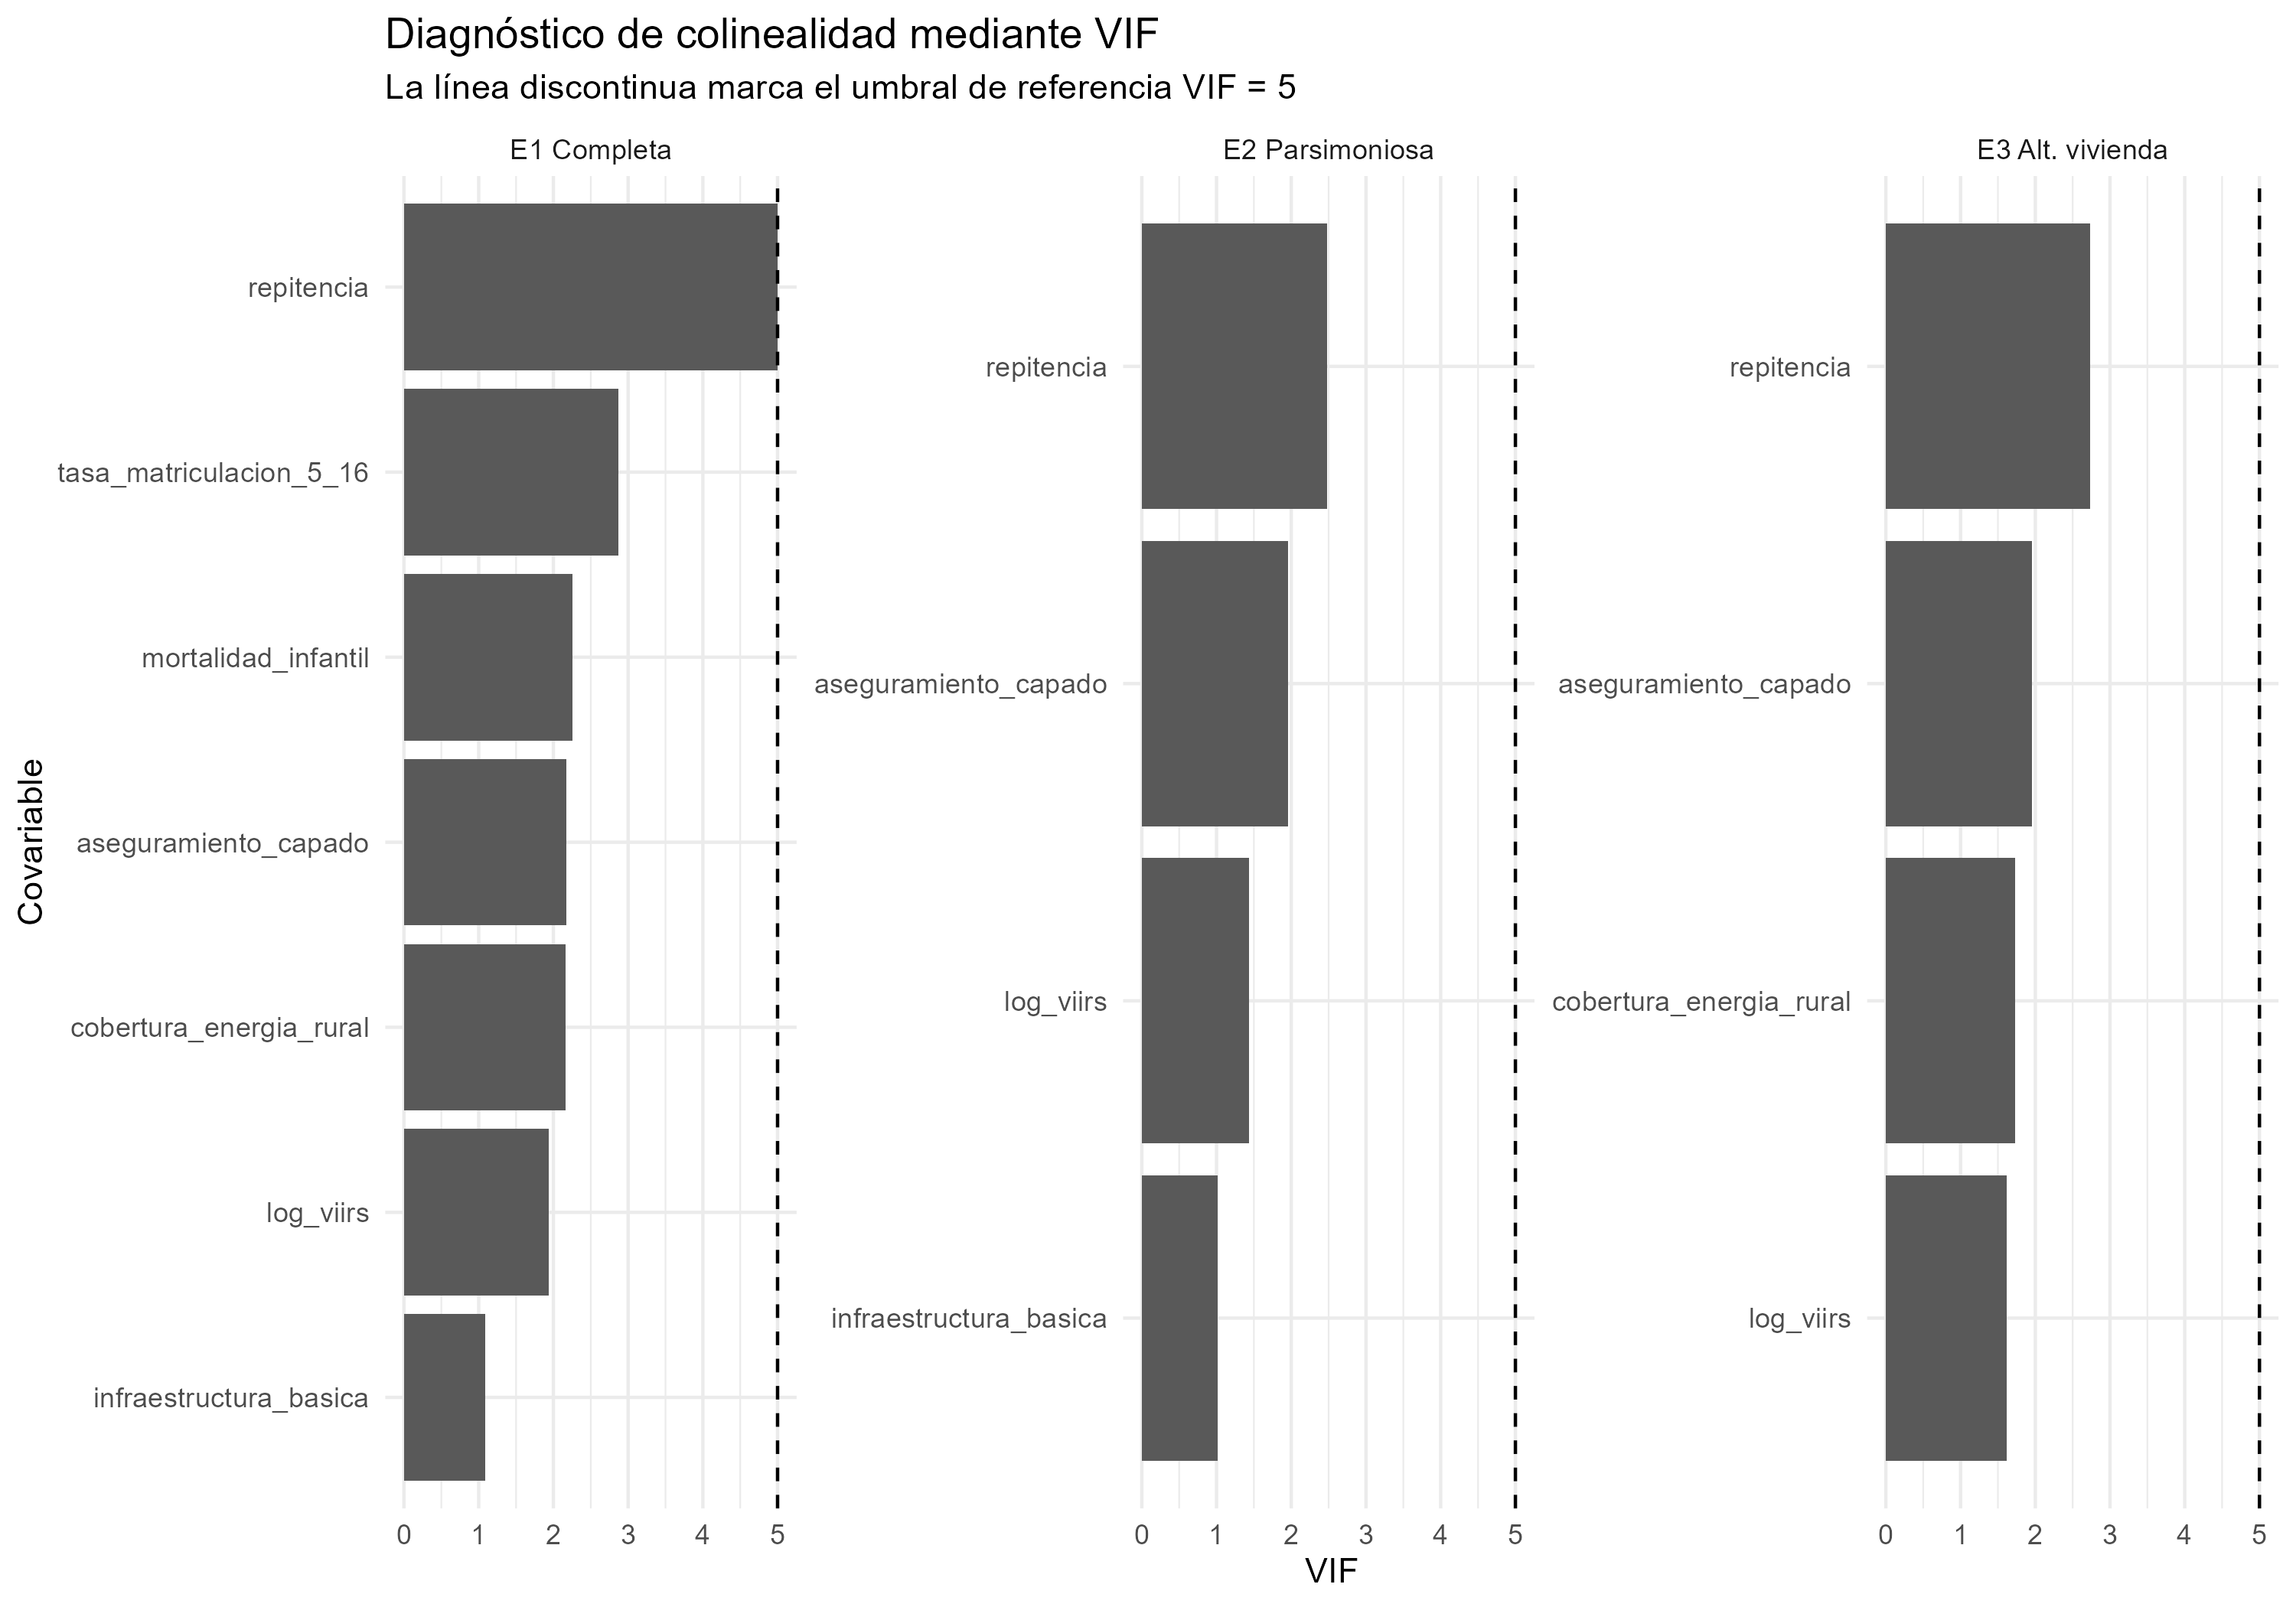
\includegraphics[width=0.95\textwidth]{fig/figures/diagnostico_VIF_escenarios.png}
\caption{Factores de inflación de la varianza por covariable y escenario.}
\label{fig:diag-VIF}
\end{figure}

La revisión de los coeficientes mostró, en términos generales, una dirección consistente con la interpretación conceptual de las covariables. La tasa de repitencia escolar presentó signo positivo en los tres escenarios, indicando una asociación directa con el IPM departamental. Por su parte, el índice de infraestructura básica, la cobertura de energía rural, el aseguramiento en salud capado y la luminosidad nocturna presentaron coeficientes negativos en los escenarios en los que fueron incorporados. La mortalidad infantil, incluida exclusivamente en el escenario Completo, presentó la dirección positiva esperada respecto a la pobreza multidimensional.

La principal excepción se observó en la tasa de matriculación de la población entre 5 y 16 años, incorporada en el escenario Completo, cuyo coeficiente fue positivo a pesar de que conceptualmente se esperaría una relación inversa con el IPM. Este comportamiento se mantuvo como una advertencia de interpretación y no se utilizó como criterio automático para eliminar la variable, en concordancia con el carácter exploratorio de esta etapa.

La Tabla~\ref{tab:ols-signos} sintetiza la dirección observada de los coeficientes en las tres especificaciones.

\begin{table}[!htbp]
\centering
\small
\caption{Dirección de los coeficientes OLS por escenario de covariables.}
\label{tab:ols-signos}
\renewcommand{\arraystretch}{1.20}
\begin{tabular}{l c c c}
\hline
\textbf{Covariable} &
\textbf{Completo} &
\textbf{Parsimonioso} &
\textbf{Alt. vivienda} \\
\hline
Repitencia escolar                    & $+$ & $+$ & $+$ \\
Matriculación 5--16 años              & $+$ & *  & *  \\
Infraestructura básica                & $-$ & $-$ & *  \\
Cobertura de energía rural            & $-$ & *  & $-$ \\
Mortalidad infantil                   & $+$ & *  & *  \\
Aseguramiento en salud capado         & $-$ & $-$ & $-$ \\
Luminosidad nocturna (log)            & $-$ & $-$ & $-$ \\
\hline
\end{tabular}

\vspace{0.2cm}
\begin{minipage}{0.90\textwidth}
\footnotesize
\textit{Nota:} Los signos indican la dirección del coeficiente estimado. El símbolo ``*'' señala que la covariable no forma parte del escenario correspondiente. Estas asociaciones se interpretan con fines diagnósticos y no como relaciones causales.
\end{minipage}
\end{table}

En conjunto, los resultados OLS evidenciaron un compromiso entre capacidad de ajuste y parsimonia. El escenario Completo explicó una mayor proporción de la variabilidad departamental observada, pero presentó una mayor carga paramétrica y una señal de colinealidad en el límite del criterio adoptado. Los escenarios Parsimonioso y Alternativo de vivienda redujeron la complejidad del ajuste y presentaron menores niveles de colinealidad, aunque con una reducción moderada del $R^2$ ajustado.

Estos resultados se utilizaron como evidencia diagnóstica sobre el comportamiento de las especificaciones y no como un procedimiento de selección automática de variables. La evaluación comparativa de las tres formulaciones se realizó posteriormente mediante la validación por exclusión de dominio y los criterios integrados definidos en la metodología.
%--------------------------------------------------------------------------------------
\section{Implementación del Modelo 1: Fay-Herriot de área}
\label{sec:res-fh}

El modelo M1 corresponde a una formulación Fay--Herriot de área calibrada a partir de los 33 dominios departamentales. En consecuencia, los resultados del ajuste, los diagnósticos internos y la validación por exclusión de dominio se interpretan a escala departamental. La salida a escala municipal se obtuvo posteriormente mediante una proyección sintética que combina el componente fijo estimado con las covariables observadas en cada municipio y el efecto aleatorio estimado para el departamento al cual pertenece la unidad. Por tanto, las estimaciones municipales presentadas para M1 no corresponden a estimaciones Fay--Herriot ajustadas directamente a nivel municipal, sino a proyecciones sintéticas derivadas del modelo de área departamental.

\subsection{Ajuste departamental y validez interna}

Los tres escenarios del modelo Fay--Herriot (M1) convergieron satisfactoriamente mediante estimación por máxima verosimilitud restringida (REML) y cumplieron las condiciones estructurales definidas para continuar con la evaluación predictiva. En todos los casos, las varianzas de muestreo asociadas a las estimaciones directas fueron finitas y estrictamente positivas, la varianza estimada del efecto aleatorio de área, $\sigma_u^2$, fue no negativa, y tanto los coeficientes estimados como los EBLUP departamentales presentaron valores finitos.

La Tabla~\ref{tab:fh-ajuste-departamental} resume los principales resultados del ajuste para los tres escenarios considerados. La varianza estimada entre áreas, $\sigma_u^2$, aumentó desde 24.3251 en el escenario Completo hasta 37.4995 en el escenario Alternativo de vivienda. Este comportamiento indica una mayor variabilidad residual entre departamentos en las especificaciones con menor número de covariables.

Por su parte, el factor de contracción promedio, $\bar{\gamma}$, presentó valores elevados en los tres escenarios, entre 0.9373 y 0.9581. Dado que valores de $\gamma$ cercanos a uno implican una mayor ponderación de la estimación directa dentro del EBLUP departamental, los resultados muestran que el modelo Fay--Herriot generó una contracción relativamente moderada hacia la componente sintética. En consecuencia, las estimaciones ajustadas conservaron una participación importante de la información proveniente de las estimaciones directas.

\begin{table}[!htbp]
\centering
\small
\caption{Resultados del ajuste departamental del modelo Fay--Herriot por escenario.}
\label{tab:fh-ajuste-departamental}
\renewcommand{\arraystretch}{1.20}
\begin{tabular}{l c c c c}
\hline
\textbf{Escenario} &
\textbf{$\sigma_u^2$} &
\textbf{$\bar{\gamma}$} &
\textbf{AIC} &
\textbf{BIC} \\
\hline
Completo          & 24.3251 & 0.9373 & 211.63 & 225.10 \\
Parsimonioso      & 33.1444 & 0.9529 & 218.31 & 227.29 \\
Alt. vivienda     & 37.4995 & 0.9581 & 222.51 & 231.49 \\
\hline
\end{tabular}
\end{table}

Dentro de la familia M1, el escenario Completo presentó los menores valores de AIC y BIC, seguido por el escenario Parsimonioso y, posteriormente, por el Alternativo de vivienda. Estos criterios se utilizaron exclusivamente para comparar las especificaciones internas del modelo Fay--Herriot, dado que los modelos M2 y M3 presentan estructuras probabilísticas y procedimientos de estimación diferentes y, por tanto, sus criterios de información no son directamente comparables con los obtenidos en M1.

Además de las condiciones estructurales anteriores, se evaluó el comportamiento de los residuos y otros supuestos asociados al ajuste mediante diagnósticos gráficos. La Figura~\ref{fig:diag-M1} presenta de manera conjunta los principales gráficos utilizados para examinar la distribución de los residuos, posibles desviaciones de normalidad, patrones sistemáticos asociados con los valores ajustados y la presencia de observaciones potencialmente influyentes.

\begin{figure}[!htbp]
\centering
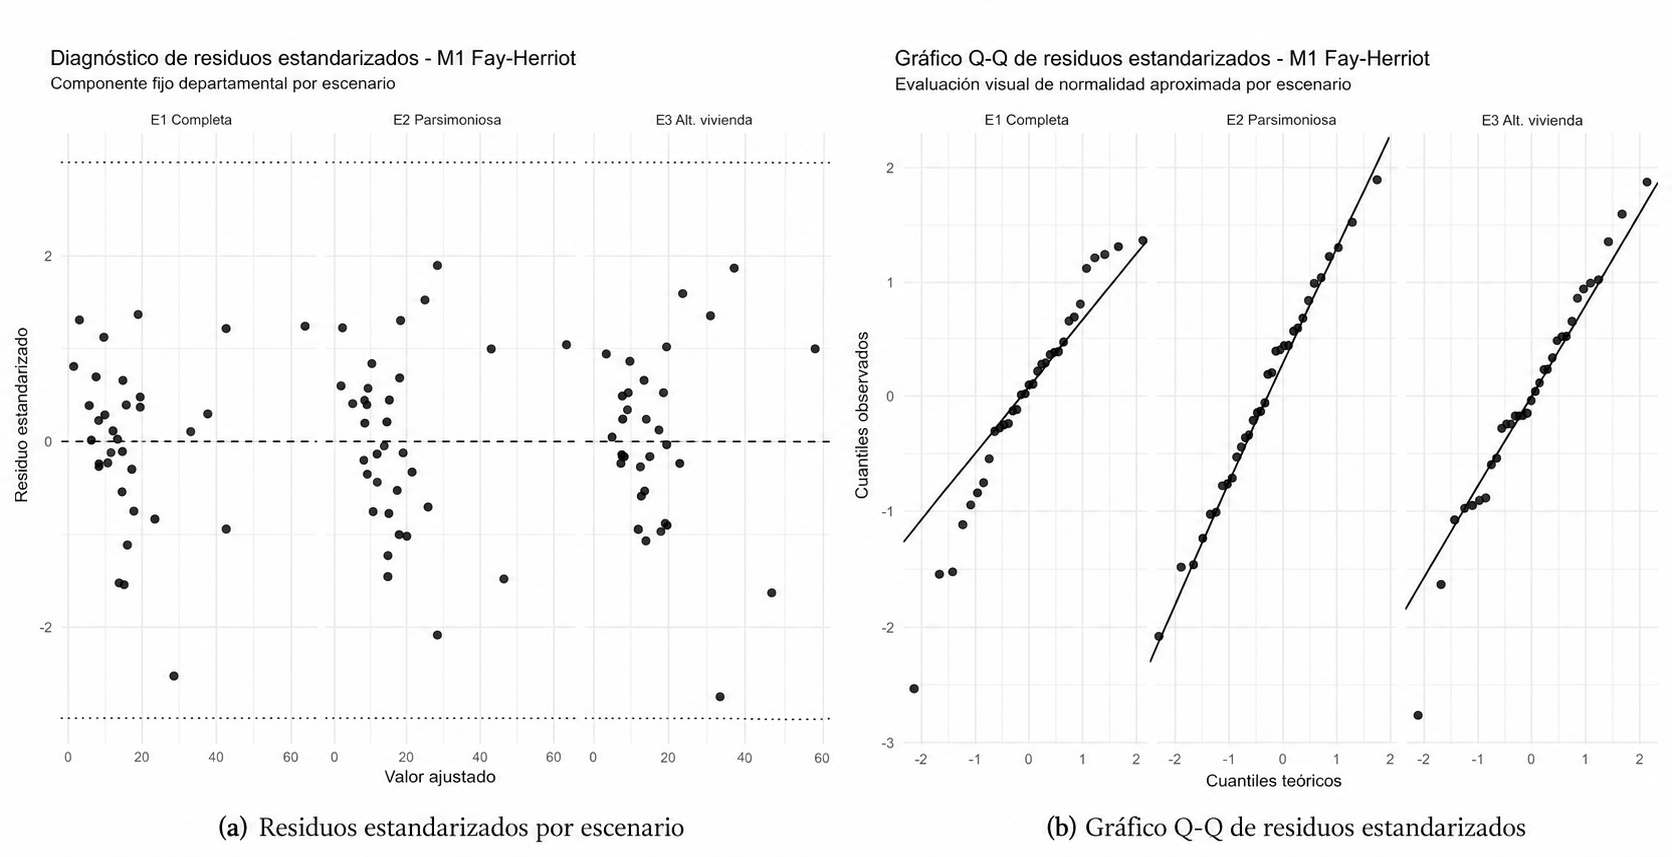
\includegraphics[width=0.95\textwidth]{fig/figures/Diagnósticos gráficos de residuos del modelo Fay–Herriot..png}
\caption{Diagnósticos gráficos de residuos del modelo Fay--Herriot.}
\label{fig:diag-M1}
\end{figure}

La evaluación formal de la validez interna incorporó diagnósticos relacionados con colinealidad entre covariables, adecuación de la forma funcional, heterocedasticidad, normalidad aproximada de los residuos estandarizados y presencia de dominios potencialmente influyentes. Los resultados se presentan en la Tabla~\ref{tab:fh-validez-interna}.

\begin{table}[!htbp]
\centering
\scriptsize
\caption{Diagnósticos de validez interna del modelo Fay--Herriot.}
\label{tab:fh-validez-interna}
\renewcommand{\arraystretch}{1.20}
\resizebox{\textwidth}{!}{
\begin{tabular}{l c c c c c c c}
\hline
\textbf{Escenario} &
\textbf{VIF máx.} &
\textbf{RESET $p$} &
\textbf{BP $p$} &
\textbf{Shapiro $p$} &
\textbf{$|r^{*}|>3$} &
\textbf{Dom. influyentes} &
\textbf{Estado} \\
\hline
Completo
& 5.005 & 0.0014 & 0.6672 & 0.1953 & 0 & 6
& Apto con advertencias \\

Parsimonioso
& 2.477 & 0.0898 & 0.0804 & 0.9965 & 0 & 7
& Apto con advertencias \\

Alt. vivienda
& 2.729 & 0.5292 & 0.0372 & 0.5821 & 0 & 6
& Apto con advertencias \\
\hline
\end{tabular}
}
\vspace{0.15cm}

\begin{minipage}{0.96\textwidth}
\footnotesize
\textit{Nota:} BP corresponde a la prueba de Breusch--Pagan y $r^{*}$ al residuo estandarizado. Los diagnósticos se interpretaron como señales de revisión y no como reglas automáticas de exclusión. La clasificación de aptitud estructural se basó en la validez de las varianzas directas, la no negatividad de $\sigma_u^2$, la finitud de los coeficientes estimados y la existencia de EBLUP finitos.
\end{minipage}
\end{table}

El escenario Completo concentró las principales advertencias relacionadas con la especificación del componente fijo. Su VIF máximo fue de 5.005, valor superior al observado en los otros dos escenarios, mientras que la prueba RESET resultó estadísticamente significativa ($p=0.0014$). Este resultado proporciona evidencia de posibles limitaciones en la forma funcional especificada y, por tanto, requiere cautela en su interpretación.

En contraste, los escenarios Parsimonioso y Alternativo de vivienda presentaron menores niveles de colinealidad, con VIF máximos de 2.477 y 2.729, respectivamente, y no mostraron evidencia estadísticamente significativa de problemas de especificación según la prueba RESET. En este sentido, ambos escenarios exhibieron un comportamiento más favorable respecto a la estructura del componente fijo.

En cuanto a la distribución de los residuos, la prueba de Shapiro--Wilk no proporcionó evidencia suficiente para rechazar el supuesto de normalidad aproximada en ninguno de los tres escenarios. De manera consistente, tampoco se identificaron residuos estandarizados con valores absolutos superiores a tres, lo que indica ausencia de observaciones extremadamente atípicas bajo este criterio.

La prueba de Breusch--Pagan tampoco mostró evidencia significativa de heterocedasticidad en los escenarios Completo y Parsimonioso. Sin embargo, en el escenario Alternativo de vivienda se obtuvo un valor $p=0.0372$, señalando posible heterocedasticidad. De acuerdo con los criterios establecidos en la metodología, este resultado se mantuvo como una advertencia diagnóstica y no constituyó por sí solo una condición automática de exclusión del escenario.

Adicionalmente, se identificaron dominios potencialmente influyentes en las tres especificaciones: seis en el escenario Completo, siete en el Parsimonioso y seis en el Alternativo de vivienda. La presencia de estos dominios justificó mantener su seguimiento durante las etapas posteriores de validación, especialmente al analizar la estabilidad de las estimaciones y el desempeño predictivo fuera de dominio.

En conjunto, los resultados de ajuste y diagnóstico muestran que los tres escenarios cumplieron las condiciones estructurales mínimas requeridas para el modelo Fay--Herriot y pudieron avanzar a la etapa de validación LODO. No obstante, ninguno se consideró completamente exento de advertencias. El escenario Completo presentó señales relacionadas principalmente con la forma funcional y la colinealidad, mientras que el escenario Alternativo de vivienda mostró evidencia de posible heterocedasticidad. Por esta razón, la selección y comparación posterior de las especificaciones no se sustentó exclusivamente en los criterios de ajuste interno, sino también en su capacidad predictiva fuera de dominio y en la coherencia global de las estimaciones.

\subsection{Desempeño predictivo departamental mediante LODO}

La capacidad predictiva fuera de dominio se evaluó excluyendo sucesivamente cada uno de los 33 departamentos y prediciéndolo a partir de los restantes. La Tabla~\ref{tab:fh-lodo} presenta las métricas obtenidas.

\begin{table}[!htbp]
\centering
\small
\caption{Desempeño predictivo LODO 2024 del modelo Fay--Herriot.}
\label{tab:fh-lodo}
\renewcommand{\arraystretch}{1.20}
\begin{tabular}{l c c c c}
\hline
\textbf{Escenario} &
\textbf{RMSE} &
\textbf{MAE} &
\textbf{Correlación} &
\textbf{$n$} \\
\hline
Completo          & 7.7047 & 5.2993 & 0.8316 & 33 \\
Parsimonioso      & 7.7563 & 5.9992 & 0.8303 & 33 \\
Alt. vivienda     & 7.8849 & 5.7569 & 0.8233 & 33 \\
\hline
\end{tabular}
\end{table}

Las diferencias de desempeño entre los tres escenarios fueron reducidas. El menor RMSE correspondió al escenario Completo, con 7.7047, seguido del Parsimonioso con 7.7563 y del Alternativo de vivienda con 7.8849. La diferencia entre el valor máximo y mínimo del RMSE fue de aproximadamente 0.18 puntos, lo que evidencia una baja sensibilidad del desempeño predictivo de M1 frente a los cambios en la especificación de covariables.

La misma estabilidad se observa en la correlación entre las estimaciones directas y las predicciones LODO, cuyos valores se ubicaron entre 0.8233 y 0.8316. Esta estabilidad no implica, sin embargo, que el modelo presente el menor error entre las tres familias evaluadas; la comparación entre M1, M2 y M3 se desarrolla posteriormente en la Sección~\ref{sec:res-comparacion}.

Debe distinguirse también el soporte de las predicciones obtenidas durante LODO del comportamiento de la proyección municipal completa. En la validación departamental, una predicción quedó fuera del intervalo 0--100 en el escenario Completo, una en el Parsimonioso y ninguna en el Alternativo de vivienda. Esta situación es independiente del número de proyecciones municipales fuera de rango, que se analiza a continuación.

\subsection{Proyección sintética municipal del IPM 2024}

Una vez ajustado el modelo departamental, se construyó una proyección sintética para los 1,121 municipios de la muestra analítica. Para cada municipio se aplicaron los coeficientes del componente fijo a sus covariables y se incorporó el efecto aleatorio estimado del departamento correspondiente. Esta operación permite trasladar la estructura calibrada a escala departamental hacia el nivel municipal, pero no modifica la naturaleza del modelo: M1 continúa siendo un modelo Fay--Herriot de área estimado con información directa departamental.

A diferencia de M2 y M3, la formulación lineal de M1 no incorpora una transformación que garantice por construcción que las proyecciones municipales permanezcan dentro del intervalo admisible del IPM. Esta limitación se hizo evidente en los tres escenarios, como se resume en la Tabla~\ref{tab:fh-proyeccion-municipal}.

\begin{table}[!htbp]
\centering
\small
\caption{Comportamiento del soporte de la proyección sintética municipal de M1.}
\label{tab:fh-proyeccion-municipal}
\renewcommand{\arraystretch}{1.20}
\begin{tabular}{l c c c c}
\hline
\textbf{Escenario} &
\textbf{$<0$} &
\textbf{$>100$} &
\textbf{Fuera de 0--100} &
\textbf{Total municipios} \\
\hline
Completo          & 197 & 2 & 199 & 1,121 \\
Parsimonioso      & 91  & 1 & 92  & 1,121 \\
Alt. vivienda     & 115 & 1 & 116 & 1,121 \\
\hline
\end{tabular}
\end{table}

El escenario Completo presentó la mayor cantidad de proyecciones municipales fuera del soporte del indicador, con 199 unidades, de las cuales 197 correspondieron a valores negativos y dos a valores superiores a 100. El escenario Parsimonioso redujo considerablemente esta situación, con 92 unidades fuera de rango, mientras que el Alternativo de vivienda presentó 116.

Estos valores no invalidan el ajuste Fay--Herriot a escala departamental, puesto que la estimación directa, la varianza de muestreo y los efectos aleatorios se definieron en ese nivel. No obstante, sí constituyen una limitación relevante de la utilización del predictor lineal como mecanismo de desagregación hacia municipios y justifican que el cumplimiento del soporte 0--100 sea evaluado explícitamente al comparar M1 con las formulaciones no lineales.

Para la comparación municipal común entre los tres modelos se utilizó el escenario Parsimonioso. Las proyecciones originales de M1 se conservaron para los análisis cuantitativos y para documentar las observaciones fuera de rango; cualquier acotamiento aplicado en la representación cartográfica tuvo únicamente fines de visualización y no alteró los valores utilizados en la evaluación estadística.

En síntesis, M1 mostró una elevada estabilidad predictiva frente a los cambios de escenario y cumplió las condiciones estructurales requeridas para el ajuste departamental. Sin embargo, la presencia de dominios influyentes y, especialmente, la existencia de proyecciones sintéticas municipales fuera del rango admisible muestran que la extrapolación del modelo de área hacia la escala municipal debe interpretarse con cautela. Estas propiedades se consideran conjuntamente con el desempeño de M2 y M3 en la comparación integrada presentada posteriormente.

%--------------------------------------------------------------------------------------
\section{Implementación del Modelo 2: desagregación municipal no lineal acotada}
\label{sec:res-m2}

El modelo M2 genera las predicciones a escala municipal mediante una transformación logística aplicada directamente sobre las covariables de cada municipio. Sin embargo, la calibración de sus parámetros se realiza utilizando como referencia las 33 estimaciones directas departamentales, obtenidas al agregar las predicciones municipales mediante los pesos poblacionales definidos en la metodología. En consecuencia, la información auxiliar entra al modelo a escala municipal, mientras que la función de verosimilitud y la validación predictiva se evalúan a escala departamental.

Esta formulación se diferencia de M1 en dos aspectos principales. En primer lugar, la transformación logística garantiza por construcción que las estimaciones municipales permanezcan dentro del intervalo admisible del IPM. En segundo lugar, el procedimiento de \textit{benchmarking} permite que, en el ajuste final, el promedio ponderado de las estimaciones municipales reproduzca numéricamente la estimación directa de cada departamento.

\subsection{Ajuste y validez interna}

Los tres escenarios alcanzaron convergencia satisfactoria y presentaron parámetros finitos. La estimación se realizó a partir de 12 puntos iniciales para cada especificación; en los tres casos, los 12 arranques fueron válidos y convergieron hacia el mismo óptimo dentro de la tolerancia establecida. Asimismo, la matriz Hessiana resultó definida positiva en las tres especificaciones, lo que aporta evidencia favorable sobre la identificación local de las soluciones obtenidas.

La desviación estándar adicional, $\tau$, presentó valores de 3.2095 en el escenario Completo, 4.5708 en el Parsimonioso y 5.3426 en el Alternativo de vivienda. Estos valores corresponden a la componente adicional de variabilidad incorporada en la función de verosimilitud, cuya varianza entra al modelo como $\tau^2$.

La Tabla~\ref{tab:m2-validez-interna} resume los principales diagnósticos de validez interna.

\begin{table}[!htbp]
\centering
\scriptsize
\caption{Diagnósticos de validez interna del modelo no lineal acotado.}
\label{tab:m2-validez-interna}
\renewcommand{\arraystretch}{1.20}
\resizebox{\textwidth}{!}{
\begin{tabular}{l c c c c c c c c}
\hline
\textbf{Escenario} &
\textbf{$\tau$} &
\textbf{Arranques válidos} &
\textbf{Hessiano PD} &
\textbf{Dom./par.} &
\textbf{Shapiro $p$} &
\textbf{$|r^{*}|>3$} &
\textbf{Benchmarking} &
\textbf{Estado} \\
\hline
Completo
& 3.2095 & 12/12 & Sí & 3.67 & 0.2883 & 0
& $3.45\times10^{-12}$
& Apto con advertencias \\

Parsimonioso
& 4.5708 & 12/12 & Sí & 5.50 & 0.1437 & 0
& $3.28\times10^{-12}$
& Apto \\

Alt. vivienda
& 5.3426 & 12/12 & Sí & 5.50 & 0.0813 & 1
& $5.04\times10^{-12}$
& Apto con advertencias \\
\hline
\end{tabular}
}

\vspace{0.15cm}
\begin{minipage}{0.96\textwidth}
\footnotesize
\textit{Nota:} PD indica que la matriz Hessiana fue definida positiva; Dom./par. corresponde a la razón entre dominios y parámetros estimados; $r^{*}$ representa el residuo departamental estandarizado previo al \textit{benchmarking}. El error de \textit{benchmarking} corresponde a la máxima diferencia absoluta entre el IPM directo departamental y el agregado ponderado de las estimaciones municipales ajustadas.
\end{minipage}
\end{table}

El escenario Completo fue clasificado como apto con advertencias debido a que la razón entre dominios y parámetros fue de 3.67, inferior al umbral de cinco dominios por parámetro utilizado como criterio diagnóstico. Esta situación refleja la mayor carga paramétrica de E1 frente al número limitado de observaciones departamentales disponibles para la calibración.

El escenario Parsimonioso no presentó advertencias internas. Los 12 arranques produjeron soluciones estables, la matriz Hessiana fue definida positiva, no se identificaron residuos estandarizados superiores a tres y la razón entre dominios y parámetros fue de 5.50.

El escenario Alternativo de vivienda también cumplió las condiciones estructurales del ajuste, aunque se identificó un residuo departamental pre-\textit{benchmarking} con valor absoluto superior a tres. La prueba de Shapiro--Wilk aplicada al conjunto de residuos estandarizados no resultó significativa ($p=0.0813$), por lo que la advertencia se interpretó como un resultado localizado y no como evidencia suficiente para descartar la especificación.

En las tres formulaciones, las covariables presentaron variación suficiente, los parámetros estimados fueron finitos y la transformación logística mantuvo todas las predicciones dentro del intervalo 0--100. Además, el error máximo de \textit{benchmarking} se ubicó en el orden de $10^{-12}$, lo que indica que la restricción de coherencia departamental se cumplió dentro de la precisión numérica del procedimiento.

La Tabla~\ref{tab:m2-soporte} presenta el rango de las estimaciones municipales finales después del \textit{benchmarking}.

\begin{table}[!htbp]
\centering
\small
\caption{Rango y coherencia de las estimaciones municipales finales de M2.}
\label{tab:m2-soporte}
\renewcommand{\arraystretch}{1.20}
\begin{tabular}{l c c c c}
\hline
\textbf{Escenario} &
\textbf{Mínimo} &
\textbf{Máximo} &
\textbf{Fuera de 0--100} &
\textbf{Error de benchmarking} \\
\hline
Completo          & 0.120 & 99.081 & 0 & $3.45\times10^{-12}$ \\
Parsimonioso      & 1.547 & 98.008 & 0 & $3.28\times10^{-12}$ \\
Alt. vivienda     & 2.360 & 97.462 & 0 & $5.04\times10^{-12}$ \\
\hline
\end{tabular}
\end{table}

Estos resultados muestran una diferencia estructural frente a M1: ninguna de las estimaciones municipales generadas por M2 requirió truncamiento posterior para respetar el soporte del IPM.

\subsection{Desempeño predictivo departamental mediante LODO}

La capacidad predictiva fuera de dominio se evaluó mediante la misma estrategia LODO aplicada a M1. En cada iteración se excluyó un departamento completo del ajuste, las covariables se estandarizaron nuevamente utilizando únicamente los municipios de entrenamiento y el dominio excluido no recibió \textit{benchmarking}. Esta última condición es fundamental, ya que aplicar el ajuste de coherencia al departamento de evaluación implicaría utilizar su propia estimación directa para construir la predicción.

Los resultados se presentan en la Tabla~\ref{tab:m2-lodo}.

\begin{table}[!htbp]
\centering
\small
\caption{Desempeño predictivo LODO 2024 del modelo no lineal acotado.}
\label{tab:m2-lodo}
\renewcommand{\arraystretch}{1.20}
\begin{tabular}{l c c c c}
\hline
\textbf{Escenario} &
\textbf{RMSE} &
\textbf{MAE} &
\textbf{Correlación} &
\textbf{$n$} \\
\hline
Completo          & 5.0971 & 3.7048 & 0.9301 & 33 \\
Parsimonioso      & 6.4540 & 4.8405 & 0.8855 & 33 \\
Alt. vivienda     & 8.4065 & 5.6452 & 0.7964 & 33 \\
\hline
\end{tabular}
\end{table}

Dentro de la familia M2, el escenario Completo presentó el menor error predictivo, con RMSE de 5.0971 y MAE de 3.7048, además de la mayor correlación entre estimaciones directas y predicciones LODO, con un valor de 0.9301. El escenario Parsimonioso presentó un desempeño intermedio, con RMSE de 6.4540, MAE de 4.8405 y correlación de 0.8855.

El escenario Alternativo de vivienda presentó el mayor error dentro de M2, con RMSE de 8.4065 y MAE de 5.6452, acompañado por una correlación inferior, de 0.7964. La diferencia entre el mayor y el menor RMSE fue de aproximadamente 3.31 puntos, lo que evidencia una sensibilidad más alta a la selección de covariables que la observada en M1.

Este resultado muestra que la mayor parsimonia no se tradujo automáticamente en un menor error predictivo dentro de M2. No obstante, la comparación entre familias de modelos se reserva para la Sección~\ref{sec:res-comparacion}, dado que el objetivo aquí es caracterizar el comportamiento interno de la formulación no lineal.

\subsection{Estimación municipal del IPM 2024}

Una vez completado el ajuste con los 33 dominios, se generaron estimaciones finales para los 1,121 municipios de la muestra analítica. A diferencia de M1, estas estimaciones se construyen directamente a partir del predictor municipal transformado mediante la función logística, por lo que el soporte del indicador se encuentra garantizado por la propia especificación funcional.

Posteriormente se aplicó el procedimiento de \textit{benchmarking} mediante un desplazamiento departamental en la escala del predictor. Este ajuste permitió que el promedio ponderado de las estimaciones municipales coincidiera, dentro de la precisión numérica, con el IPM directo del departamento correspondiente sin alterar la propiedad de acotamiento.

Por esta razón, el \textit{benchmarking} debe interpretarse como un procedimiento de coherencia estructural de la estimación final y no como evidencia de capacidad predictiva. La capacidad de generalización del modelo se evaluó de manera independiente mediante LODO, donde el departamento excluido no recibió este ajuste.

Para la comparación municipal común con M1 y M3 se utilizó el escenario Parsimonioso. Bajo esta especificación, las estimaciones municipales de M2 se ubicaron entre 1.547 y 98.008 puntos del IPM y no se presentaron valores fuera del intervalo admisible.

La comparación posterior con M3 bajo el mismo escenario mostró una correlación municipal de 0.9901 y una diferencia absoluta media de 1.69 puntos porcentuales. Estas medidas se interpretan como indicadores de concordancia entre formulaciones y no como métricas de precisión municipal, dado que no se dispone de una estimación directa municipal del IPM 2024 que pueda utilizarse como referencia observada.

En síntesis, M2 presentó estabilidad numérica en los tres escenarios, cumplimiento exacto de las restricciones de soporte y coherencia departamental, y un desempeño predictivo que varió de manera apreciable según la especificación de covariables. El escenario Completo alcanzó el menor error LODO dentro de esta familia, mientras que el escenario Parsimonioso presentó la estructura interna más limpia al no registrar advertencias diagnósticas. Estas diferencias se incorporan posteriormente en la comparación integrada de las tres formulaciones.
%--------------------------------------------------------------------------------------
\section{Implementación del Modelo 3: desagregación espacial CAR}
\label{sec:res-m3}

El modelo M3 extiende la formulación no lineal acotada de M2 mediante la incorporación de un componente espacial municipal con estructura condicional autorregresiva (CAR) de rango reducido. Al igual que en M2, las covariables ingresan al modelo a escala municipal, las predicciones se transforman mediante una función logística y la calibración de los parámetros se realiza utilizando como referencia las 33 estimaciones directas departamentales.

La principal diferencia respecto a M2 radica en la inclusión de un efecto espacial construido a partir de la estructura de vecindad municipal. Este componente se representó mediante seis patrones espaciales de rango reducido, obtenidos a partir de la matriz de contigüidad tipo Reina, con el propósito de incorporar dependencia territorial sin estimar un efecto independiente para cada uno de los 1,121 municipios.

\subsection{Ajuste, validez interna y sensibilidad espacial}

Durante las etapas preliminares de estimación del modelo espacial CAR de rango reducido (M3) se exploró la estimación libre del parámetro de dependencia espacial, $\rho$. Sin embargo, las soluciones obtenidas se concentraron repetidamente en los límites del intervalo de búsqueda: inicialmente alrededor de $-0.95$ y, posteriormente, cerca de $0.95$ bajo una parametrización alternativa. Este comportamiento sugirió una identificación limitada de $\rho$ cuando su estimación se sustenta únicamente en la información agregada de los 33 dominios departamentales utilizados para la calibración.

En consecuencia, se optó por tratar $\rho$ como un parámetro de sensibilidad en lugar de estimarlo libremente dentro del modelo final. Para ello, se evaluaron cuatro valores predefinidos:

\[
\rho \in \{0.25,\;0.50,\;0.75,\;0.90\}.
\]

Se estableció $\rho=0.50$ como especificación de referencia para la comparación principal de M3, mientras que los demás valores se utilizaron para examinar la estabilidad de los parámetros estimados y de las predicciones municipales frente a distintos niveles de dependencia espacial impuesta.

Bajo la especificación de referencia, los tres escenarios considerados alcanzaron convergencia satisfactoria. Para cada escenario se utilizaron ocho puntos iniciales y, en todos los casos, los ocho arranques fueron válidos y convergieron hacia el mismo óptimo dentro de la tolerancia establecida. Asimismo, la matriz Hessiana resultó definida positiva y la matriz de precisión asociada a la estructura CAR permaneció válida, proporcionando evidencia favorable sobre la estabilidad numérica de la estimación.

La Tabla~\ref{tab:m3-validez-interna} resume los principales diagnósticos internos obtenidos para el modelo espacial con $\rho=0.50$.

\begin{table}[!htbp]
\centering
\scriptsize
\caption{Diagnósticos de validez interna del modelo espacial CAR de rango reducido con $\rho=0.50$.}
\label{tab:m3-validez-interna}
\renewcommand{\arraystretch}{1.20}
\resizebox{\textwidth}{!}{
\begin{tabular}{l c c c c c c c c}
\hline
\textbf{Escenario} &
\textbf{$\tau$} &
\textbf{DE efecto espacial} &
\textbf{Moran $I$} &
\textbf{$p$ Moran} &
\textbf{Arranques válidos} &
\textbf{Hessiano PD} &
\textbf{$|r^{*}|>3$} &
\textbf{Estado} \\
\hline
Completo
& 2.0993 & 0.2501 & 0.9883 & 0.001
& 8/8 & Sí & 0
& Apto con advertencias \\

Parsimonioso
& 2.5584 & 0.3257 & 0.9935 & 0.001
& 8/8 & Sí & 0
& Apto con advertencias \\

Alt. vivienda
& 3.9040 & 0.3391 & 0.9966 & 0.001
& 8/8 & Sí & 0
& Apto con advertencias \\
\hline
\end{tabular}
}

\vspace{0.15cm}
\begin{minipage}{0.96\textwidth}
\footnotesize
\textit{Nota:} PD indica que la matriz Hessiana fue definida positiva; DE corresponde a la desviación estándar del efecto espacial municipal; $r^{*}$ representa el residuo departamental estandarizado previo al \textit{benchmarking}. El estadístico global de Moran se calculó sobre el efecto espacial municipal estimado y no sobre los residuos finales del modelo.
\end{minipage}
\end{table}

La desviación estándar departamental adicional, $\tau$, fue de 2.0993 en el escenario Completo, 2.5584 en el escenario Parsimonioso y 3.9040 en el escenario Alternativo de vivienda. Este incremento indica que, bajo las especificaciones más reducidas, una mayor proporción de la variabilidad departamental no explicada por las covariables debió ser absorbida por el componente aleatorio adicional del modelo.

De manera similar, la desviación estándar del efecto espacial municipal aumentó desde 0.2501 en el escenario Completo hasta 0.3391 en el Alternativo de vivienda. Estas diferencias reflejan variaciones en la magnitud del componente territorial requerido por cada especificación para representar la heterogeneidad espacial no capturada por el componente fijo.

El efecto espacial estimado presentó una autocorrelación positiva elevada en los tres escenarios. El índice global de Moran varió entre 0.9883 y 0.9966, con valores $p=0.001$ en todos los casos. Este resultado indica que el componente espacial retenido por la representación CAR de rango reducido conserva una estructura geográfica fuertemente organizada y coherente con la matriz de vecindad utilizada en el modelo.

No obstante, estos valores deben interpretarse con cautela. El índice de Moran fue calculado sobre el propio efecto espacial estimado y, por tanto, no constituye una prueba de ausencia de autocorrelación en los residuos finales. Su función en este contexto es caracterizar la organización espacial del componente territorial incorporado por el modelo, mientras que la evaluación de la autocorrelación residual corresponde a un diagnóstico diferente.

La Figura~\ref{fig:diag-Moran} presenta gráficamente esta relación mediante el diagrama de Moran del efecto espacial municipal estimado.

\begin{figure}[!htbp]
\centering
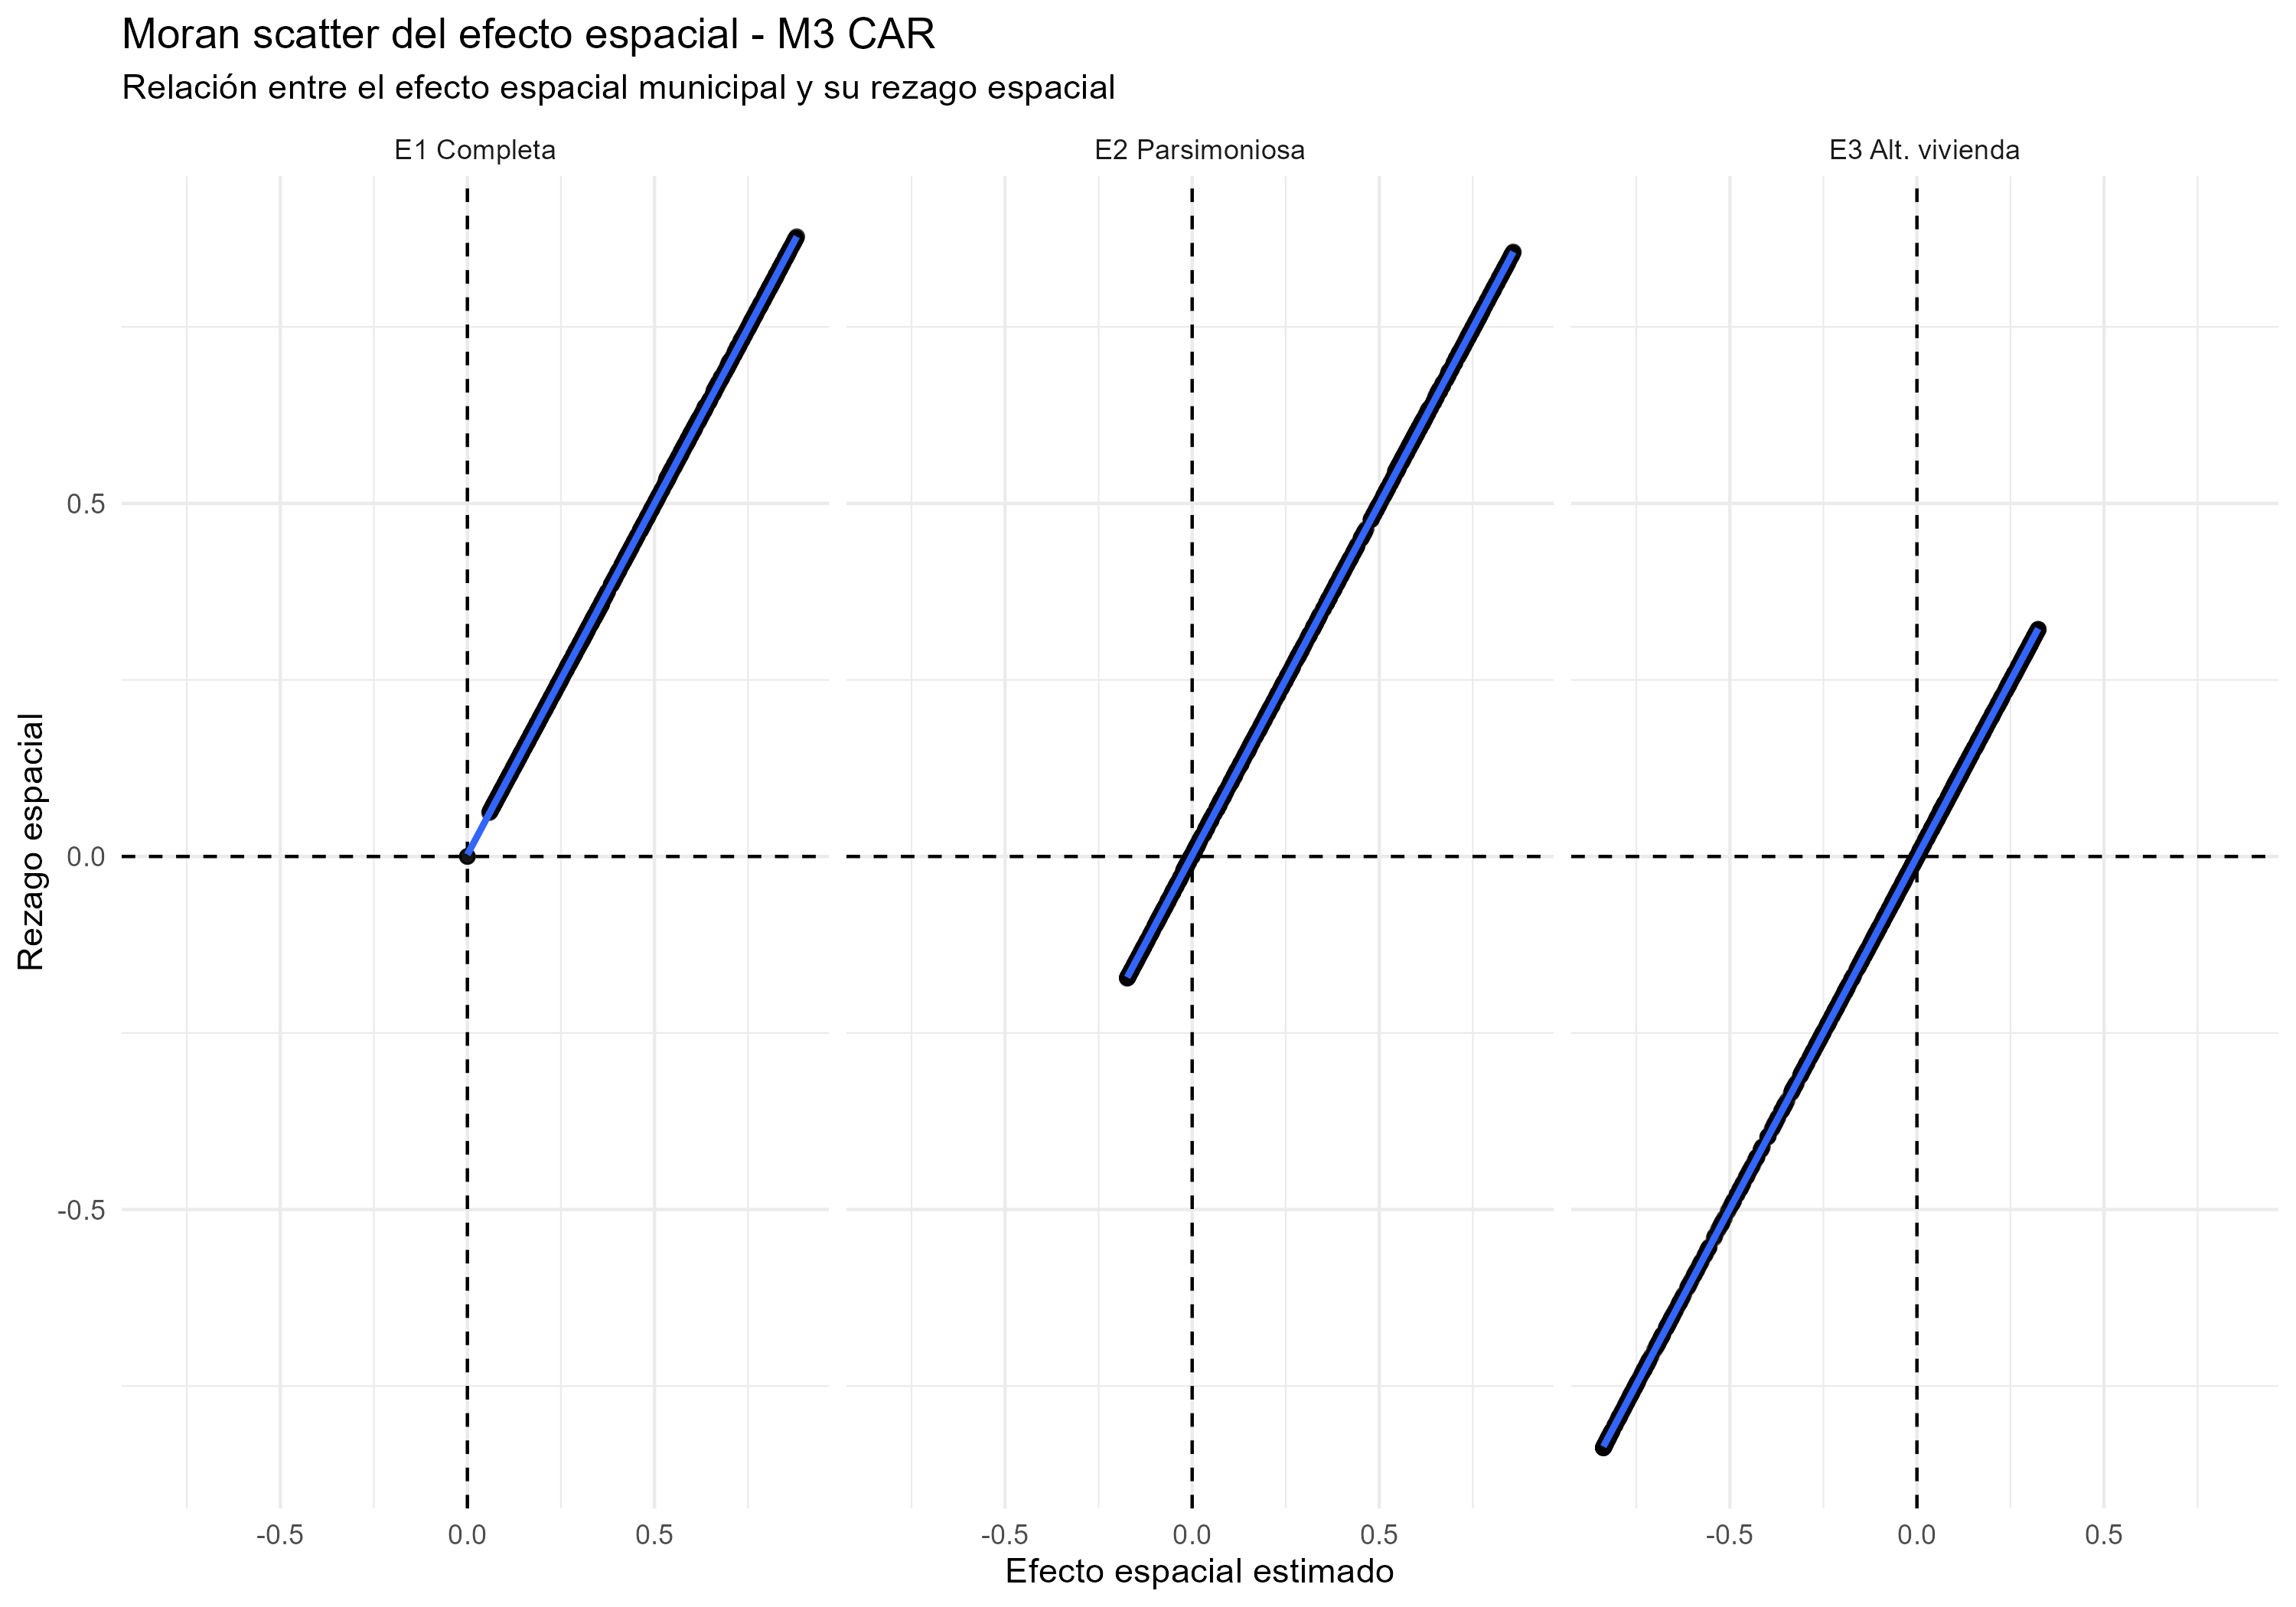
\includegraphics[width=0.95\textwidth]{fig/figures/diagnostico_M3_Moran_efecto_espacial.png}
\caption{Diagrama de Moran del efecto espacial municipal estimado por el modelo CAR.}
\label{fig:diag-Moran}
\end{figure}

En relación con los residuos departamentales previos al \textit{benchmarking}, no se identificaron valores estandarizados con valor absoluto superior a tres en ninguno de los escenarios. Este resultado indica que, bajo este criterio, no se observaron desviaciones extremas en los residuos utilizados para evaluar la consistencia interna del ajuste.

Las principales advertencias asociadas a M3 estuvieron relacionadas con la estructura de la red espacial municipal. Bajo el criterio de contigüidad tipo Reina, dos unidades insulares no presentaron vecinos directos y la red espacial quedó conformada inicialmente por tres componentes conexos. Estas particularidades, descritas previamente en la sección de preprocesamiento espacial, fueron tratadas explícitamente durante la construcción de la matriz de vecindad y se conservaron como advertencias metodológicas. Su presencia no implicó la eliminación de municipios ni la modificación del universo de estimación.

Con base en estos resultados, los tres escenarios cumplieron las condiciones mínimas de validez interna definidas para el modelo M3. La convergencia consistente entre múltiples puntos iniciales, la existencia de Hessianos definidos positivos, la validez de la matriz de precisión espacial y la ausencia de residuos departamentales extremos proporcionaron evidencia favorable sobre la estabilidad del procedimiento de estimación, aunque las particularidades de conectividad de la red espacial justificaron mantener la clasificación de ``apto con advertencias''.

Finalmente, se evaluó la sensibilidad de los resultados frente al valor fijado de $\rho$. Al variar el parámetro entre 0.25 y 0.90, los cambios observados en $\tau$, en la desviación estándar del efecto espacial y en los valores extremos de las predicciones municipales fueron reducidos. Asimismo, las estimaciones municipales se mantuvieron dentro del intervalo teórico de 0 a 100 para todos los valores analizados.

El procedimiento de \textit{benchmarking} también conservó su exactitud numérica en toda la grilla de sensibilidad. En consecuencia, los principales resultados de M3 mostraron estabilidad frente a variaciones moderadas y altas del parámetro $\rho$ dentro del rango evaluado. Esto respalda el uso de $\rho=0.50$ como especificación de referencia para la comparación principal, sin interpretar dicho valor como una estimación empírica única o identificada directamente a partir de los datos.

\subsection{Desempeño predictivo departamental mediante LODO}

La capacidad predictiva fuera de dominio se evaluó mediante la misma estrategia LODO utilizada para M1 y M2. En cada iteración, el departamento excluido no participó en la estimación de los parámetros ni recibió \textit{benchmarking}. La estandarización de las covariables se recalculó utilizando únicamente los municipios pertenecientes a los dominios de entrenamiento.

La información geográfica y la estructura de vecindad del dominio excluido permanecieron disponibles durante la predicción, dado que constituyen información auxiliar externa y no forman parte de la respuesta directa utilizada para la evaluación.

Los resultados de la validación se presentan en la Tabla~\ref{tab:m3-lodo}.

\begin{table}[!htbp]
\centering
\small
\caption{Desempeño predictivo LODO 2024 del modelo espacial CAR de rango reducido con $\rho=0.50$.}
\label{tab:m3-lodo}
\renewcommand{\arraystretch}{1.20}
\begin{tabular}{l c c c c}
\hline
\textbf{Escenario} &
\textbf{RMSE} &
\textbf{MAE} &
\textbf{Correlación} &
\textbf{$n$} \\
\hline
Completo          & 6.0406  & 4.4623 & 0.9001 & 33 \\
Parsimonioso      & 4.7197  & 3.6731 & 0.9410 & 33 \\
Alt. vivienda     & 10.4274 & 6.5350 & 0.7063 & 33 \\
\hline
\end{tabular}
\end{table}

Dentro de la familia M3, el escenario Parsimonioso presentó el menor error predictivo, con un RMSE de 4.7197 y un MAE de 3.6731, acompañado por la mayor correlación entre las estimaciones directas y las predicciones LODO, con un valor de 0.9410.

El escenario Completo mostró un desempeño intermedio, con RMSE de 6.0406, MAE de 4.4623 y correlación de 0.9001. En contraste, el escenario Alternativo de vivienda presentó un deterioro importante del desempeño predictivo, alcanzando un RMSE de 10.4274, un MAE de 6.5350 y una correlación de 0.7063.

La diferencia entre el mayor y el menor RMSE fue aproximadamente de 5.71 puntos, la mayor variación observada entre escenarios dentro de las tres familias de modelos. Este resultado indica que la formulación espacial es particularmente sensible al conjunto de covariables utilizado y que la incorporación de dependencia espacial no compensa automáticamente una especificación auxiliar menos favorable.

La comparación directa de este desempeño con M1 y M2 se presenta posteriormente en la Sección~\ref{sec:res-comparacion}, con el propósito de mantener separada la evaluación interna de M3 de la comparación integrada entre formulaciones.

\subsection{Estimación municipal del IPM 2024}

Una vez completada la calibración con los 33 dominios departamentales, se obtuvieron estimaciones para los 1,121 municipios de la muestra analítica. Al igual que en M2, el predictor municipal se transformó mediante una función logística, por lo que las estimaciones permanecieron dentro del intervalo admisible del IPM.

Para la estimación final se utilizó el escenario Parsimonioso con $\rho=0.50$, especificación adoptada como referencia común para la comparación municipal entre M1, M2 y M3. Posteriormente se aplicó el mismo procedimiento de \textit{benchmarking} utilizado en M2, mediante un desplazamiento departamental sobre la escala del predictor.

Después de este ajuste, las estimaciones municipales bajo E2 se ubicaron aproximadamente entre 0.96 y 99.20 puntos del IPM. No se identificaron valores inferiores a cero ni superiores a 100 y el agregado ponderado de las estimaciones municipales reprodujo, dentro de la precisión numérica, el IPM directo correspondiente a cada departamento.

Al igual que en M2, el \textit{benchmarking} se interpreta exclusivamente como una condición de coherencia estructural de la estimación final y no como evidencia de capacidad predictiva. La evaluación de generalización del modelo corresponde a los resultados LODO obtenidos sin utilizar la estimación directa del departamento excluido.

Bajo el escenario Parsimonioso, M3 presentó una elevada concordancia con las estimaciones municipales de M2. La correlación entre ambas formulaciones fue de 0.9901 y la diferencia absoluta media alcanzó 1.69 puntos porcentuales. La correlación entre M3 y la proyección sintética municipal de M1 fue de 0.9374. Estas medidas describen la similitud entre las distribuciones municipales producidas por los modelos, pero no constituyen medidas de precisión municipal.

En síntesis, M3 presentó estabilidad numérica en los tres escenarios, una estructura espacial claramente definida, cumplimiento del soporte 0--100 y coherencia departamental mediante \textit{benchmarking}. Su desempeño predictivo, sin embargo, mostró una sensibilidad considerable a la especificación de covariables: el escenario Parsimonioso presentó el menor error dentro de la familia, mientras que el Alternativo de vivienda mostró un deterioro sustancial. Estos resultados evidencian que el aporte del componente espacial depende de su interacción con la información auxiliar incorporada y deben interpretarse conjuntamente con las otras dos formulaciones en la comparación integrada.
%--------------------------------------------------------------------------------------
\section{Comparación integrada y producción cartográfica}
\label{sec:res-comparacion}

Una vez caracterizadas por separado las propiedades internas y el desempeño predictivo de M1, M2 y M3, se realizó una comparación integrada bajo condiciones comunes. Las nueve combinaciones de modelo y escenario superaron las condiciones mínimas establecidas para participar en esta etapa: completaron los 33 dominios de la validación \textit{Leave-One-Domain-Out} (LODO) y produjeron métricas de evaluación finitas.

Para garantizar la comparabilidad entre formulaciones, el RMSE, el MAE y la correlación LODO se calcularon sobre exactamente los mismos 33 dominios departamentales y mediante la misma estrategia de exclusión sucesiva en las nueve combinaciones evaluadas. En cada iteración, la estimación directa del departamento excluido permaneció fuera del proceso de ajuste y no se utilizó para construir su predicción.

La comparación entre familias se realizó exclusivamente con las métricas obtenidas mediante el mismo esquema LODO 2024. Los criterios de ajuste interno, como AIC, BIC o la función objetivo penalizada, no se utilizaron para ordenar modelos pertenecientes a familias probabilísticas diferentes, sino únicamente como diagnósticos internos de las especificaciones correspondientes.

\subsection{Comparación del desempeño predictivo}

La Tabla~\ref{tab:comparacion-m123} consolida el RMSE, MAE y la correlación entre las estimaciones directas departamentales y las predicciones LODO obtenidas para las nueve combinaciones evaluadas.

\begin{table}[!htbp]
\centering
\small
\caption{Comparación controlada del desempeño predictivo de M1, M2 y M3 mediante LODO 2024.}
\label{tab:comparacion-m123}
\renewcommand{\arraystretch}{1.20}
\begin{tabular}{l l c c c}
\hline
\textbf{Escenario} &
\textbf{Modelo} &
\textbf{RMSE} &
\textbf{MAE} &
\textbf{Correlación} \\
\hline
Completo
& M1 Fay--Herriot
& 7.7047 & 5.2993 & 0.8316 \\

Completo
& M2 no lineal
& 5.0971 & 3.7048 & 0.9301 \\

Completo
& M3 CAR
& 6.0406 & 4.4623 & 0.9001 \\
\hline
Parsimonioso
& M1 Fay--Herriot
& 7.7563 & 5.9992 & 0.8303 \\

Parsimonioso
& M2 no lineal
& 6.4540 & 4.8405 & 0.8855 \\

Parsimonioso
& M3 CAR
& 4.7197 & 3.6731 & 0.9410 \\
\hline
Alt. vivienda
& M1 Fay--Herriot
& 7.8849 & 5.7569 & 0.8233 \\

Alt. vivienda
& M2 no lineal
& 8.4065 & 5.6452 & 0.7964 \\

Alt. vivienda
& M3 CAR
& 10.4274 & 6.5350 & 0.7063 \\
\hline
\end{tabular}
\end{table}

La comparación por escenario muestra que ninguna familia presentó sistemáticamente el menor error bajo todas las especificaciones de covariables. En el escenario Completo, M2 alcanzó el menor RMSE (5.0971), seguido por M3 (6.0406) y M1 (7.7047). Bajo el escenario Parsimonioso, M3 presentó el menor RMSE de las nueve combinaciones evaluadas (4.7197), acompañado por el menor MAE (3.6731) y la mayor correlación LODO (0.9410). En el escenario Alternativo de vivienda, M1 presentó el menor RMSE (7.8849), aunque las diferencias con M2 fueron más reducidas que las observadas frente a M3.

Por tanto, la incorporación de un componente espacial no produjo una mejora automática del desempeño predictivo. Su aporte dependió de la interacción entre la estructura espacial y el conjunto de covariables utilizado. En particular, M3 mostró un comportamiento favorable bajo el escenario Parsimonioso, pero un deterioro considerable bajo el Alternativo de vivienda.

La combinación M3--Parsimonioso redujo el RMSE aproximadamente en un 7.4\,\% respecto a M2--Completo, que presentó el segundo menor RMSE entre las nueve combinaciones. Esta diferencia se interpreta como una comparación descriptiva del desempeño predictivo observado y no como evidencia suficiente, por sí sola, para seleccionar una formulación únicamente a partir de una métrica.

Las diferencias en el desempeño predictivo entre modelos y escenarios se presentan visualmente en los gráficos de la figura~\ref{fig:comparacion-desmp-predict}. Cada figura muestra, respectivamente, el RMSE, el MAE y la correlación obtenidos mediante la validación LODO para las nueve combinaciones evaluadas, facilitando la comparación tanto entre formulaciones como entre escenarios de covariables.

\begin{figure}[!htbp]
\centering
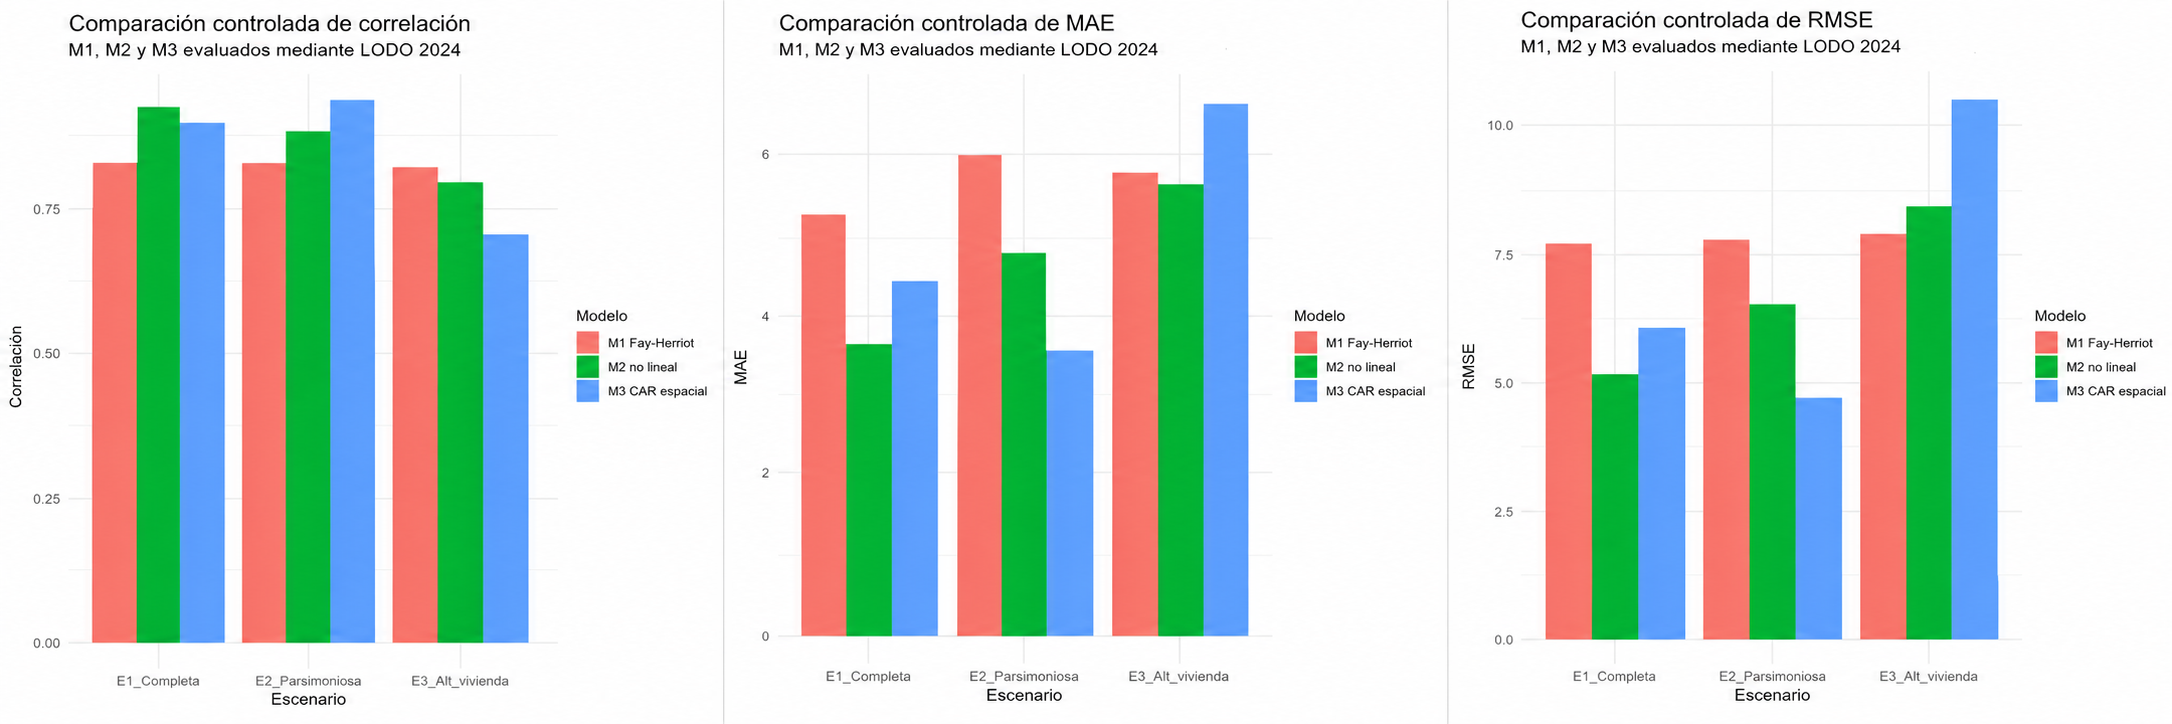
\includegraphics[width=0.95\textwidth]{fig/figures/Comparacion_Desemp_predict.png}
\caption{Comparación del desempeño predictivo de los modelos M1, M2 y M3.}
\label{fig:comparacion-desmp-predict}
\end{figure}

\subsection{Estabilidad frente a los escenarios de covariables}

Además del nivel de error, se examinó la estabilidad de cada familia frente a los cambios en la especificación auxiliar. M1 presentó la menor amplitud de RMSE entre escenarios, con una diferencia de 0.18 puntos entre su valor mínimo y máximo. En M2, esta amplitud aumentó a 3.31 puntos, mientras que M3 alcanzó 5.71 puntos.

Estos resultados muestran que M1 fue relativamente estable frente a las modificaciones del conjunto de covariables, aunque presentó un nivel de error LODO comparativamente similar en los tres escenarios. M2 mostró una sensibilidad intermedia, mientras que M3 presentó la mayor dependencia respecto a la especificación auxiliar.

Tomando únicamente el menor RMSE dentro de cada familia como resumen descriptivo, las formulaciones de referencia fueron el escenario Completo para M1 (RMSE = 7.7047), el escenario Completo para M2 (RMSE = 5.0971) y el escenario Parsimonioso para M3 (RMSE = 4.7197). Esta identificación se utiliza para describir el comportamiento interno de cada familia y no implica que un único escenario deba adoptarse como referencia para todas las comparaciones posteriores.

La comparación integrada también mostró diferencias en las propiedades garantizadas por cada formulación. M1 se estimó como un modelo Fay--Herriot a escala departamental y posteriormente produjo una proyección sintética municipal. Debido a su estructura lineal, esta proyección no garantiza el soporte 0--100 del IPM: en el ajuste final se identificaron 199, 92 y 116 proyecciones municipales fuera de rango bajo los escenarios Completo, Parsimonioso y Alternativo de vivienda, respectivamente.

M2 y M3, en cambio, incorporaron una transformación logística en la propia formulación municipal. En consecuencia, no produjeron estimaciones municipales fuera del intervalo admisible en ninguno de los tres escenarios. Adicionalmente, ambas formulaciones aplicaron un procedimiento de \textit{benchmarking} que garantizó que el promedio ponderado de las estimaciones municipales reprodujera la estimación directa departamental dentro de la precisión numérica.

Estas diferencias deben interpretarse separadamente de las métricas LODO. El cumplimiento del rango y del \textit{benchmarking} constituye evidencia de coherencia estructural de las estimaciones finales, mientras que RMSE, MAE y correlación LODO evalúan la capacidad predictiva fuera de dominio.

\subsection{Concordancia de las estimaciones municipales}

Para comparar las distribuciones municipales producidas por las tres formulaciones se utilizó el escenario Parsimonioso como especificación común. Su utilización en esta etapa responde a la necesidad de comparar los modelos bajo el mismo conjunto de covariables y no a una selección automática de este escenario como superior para todas las familias.

La Tabla~\ref{tab:concordancia-e2} presenta la correlación entre estimaciones municipales y la diferencia absoluta media para cada par de modelos.

\begin{table}[!htbp]
\centering
\small
\caption{Concordancia entre las estimaciones municipales de M1, M2 y M3 bajo el escenario Parsimonioso.}
\label{tab:concordancia-e2}
\renewcommand{\arraystretch}{1.20}
\begin{tabular}{l c c}
\hline
\textbf{Comparación} &
\textbf{Correlación} &
\textbf{Diferencia absoluta media} \\
\hline
M1--M2 & 0.9511 & 3.22 p.p. \\
M1--M3 & 0.9374 & 3.73 p.p. \\
M2--M3 & 0.9901 & 1.69 p.p. \\
\hline
\end{tabular}

\vspace{0.15cm}
\begin{minipage}{0.94\textwidth}
\footnotesize
\textit{Nota:} p.p. = puntos porcentuales. Estas medidas expresan concordancia entre formulaciones y no precisión municipal, dado que no se dispone de una estimación directa municipal del IPM 2024 que pueda utilizarse como referencia observada.
\end{minipage}
\end{table}

La mayor concordancia se observó entre M2 y M3, con una correlación de 0.9901 y una diferencia absoluta media de 1.69 puntos porcentuales. Esto indica que la incorporación del componente CAR produjo ajustes territoriales sobre una estructura municipal ampliamente similar a la obtenida mediante M2.

Las comparaciones que involucraron a M1 presentaron diferencias mayores. La correlación M1--M2 fue de 0.9511, con una diferencia absoluta media de 3.22 puntos porcentuales, mientras que M1--M3 alcanzó una correlación de 0.9374 y una diferencia absoluta media de 3.73 puntos. Este comportamiento es coherente con las diferencias en la arquitectura de los modelos: M1 se calibra a escala departamental y posteriormente genera una proyección sintética utilizando las covariables municipales y el efecto aleatorio del departamento, mientras que M2 y M3 incorporan la estructura municipal directamente dentro de sus respectivas formulaciones de desagregación.

\subsection{Producción cartográfica}

Con fines de comparación territorial, se produjo cartografía municipal de las tres formulaciones bajo el escenario Parsimonioso. Se utilizó una clasificación común para facilitar la comparación visual entre modelos.

En el caso de M1, la representación corresponde a la proyección sintética municipal derivada del modelo Fay--Herriot departamental. En M2 y M3, los mapas representan las estimaciones municipales finales posteriores al procedimiento de \textit{benchmarking}. Para M3 se utilizó la especificación espacial de referencia con $\rho=0.50$.

\begin{figure}[!htbp]
\centering
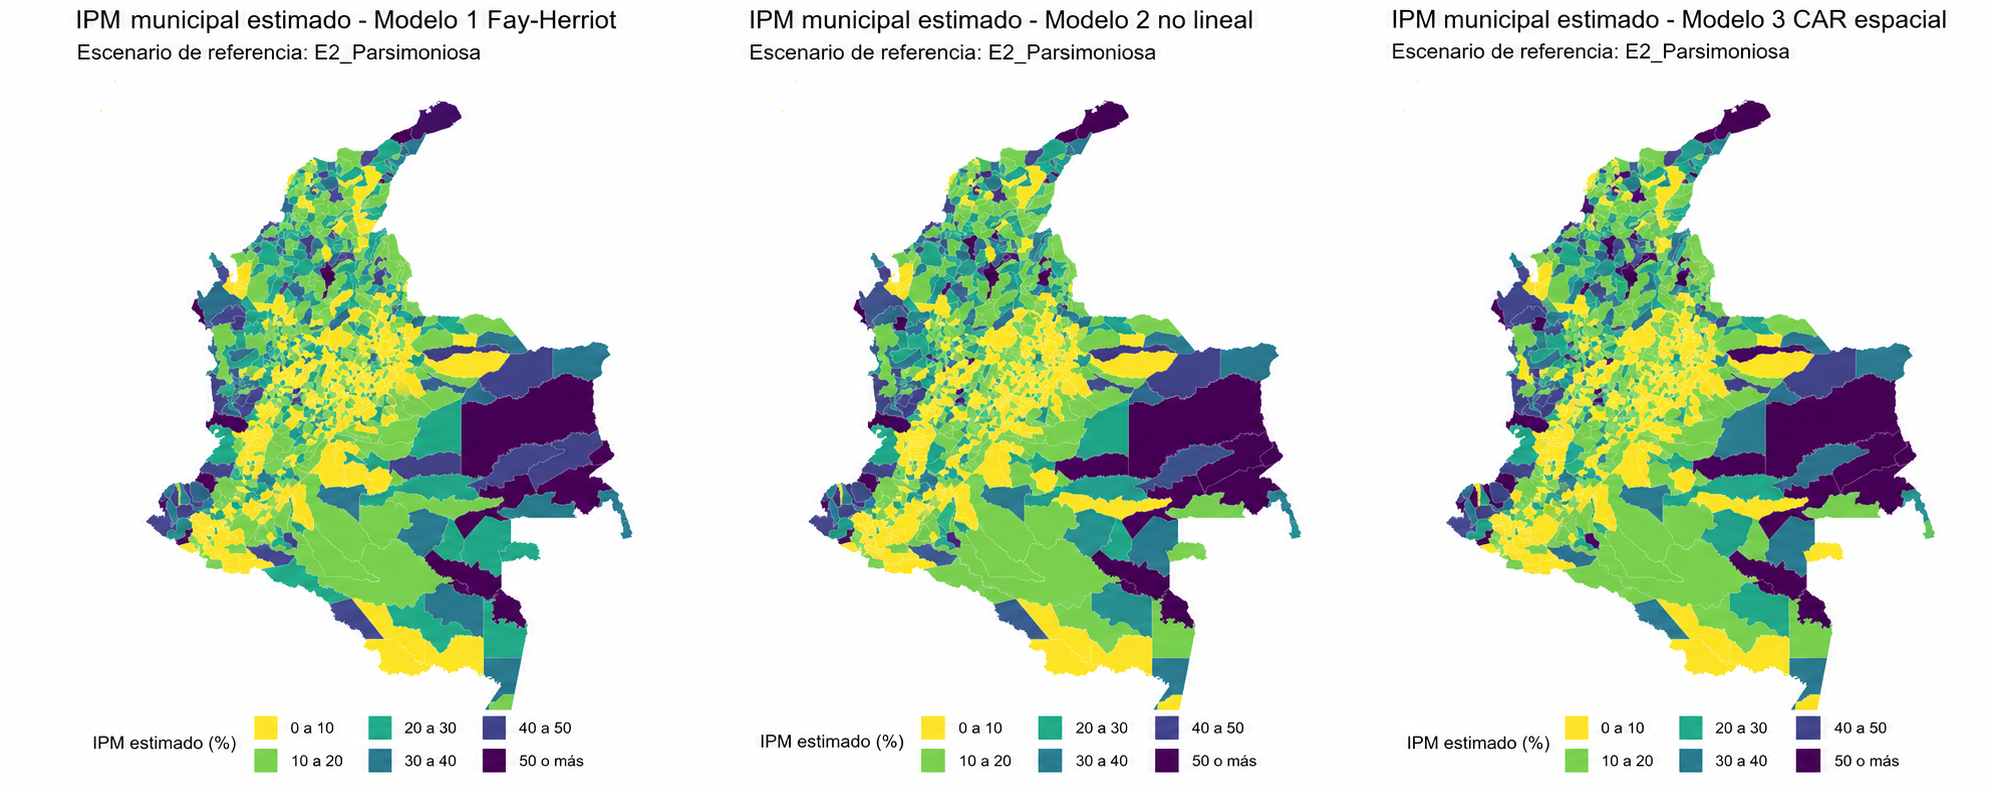
\includegraphics[width=0.95\textwidth]{fig/figures/Panel_Horizontal_Mapas_M1_M2_M3.png}
\caption{Estimación municipal del IPM 2024 bajo el modelo de Fay-Herriot, escenario Parsimonioso.}
\label{fig:Comparacion_Mapas}
\end{figure}

La cartografía permite examinar la distribución territorial generada por cada formulación y complementar las medidas numéricas de concordancia. La proximidad observada entre M2 y M3 en la Tabla~\ref{tab:concordancia-e2} es consistente con la similitud general de sus patrones territoriales, aunque el componente espacial de M3 introduce modificaciones locales asociadas a la estructura de vecindad.

En todos los casos, los mapas tienen una función descriptiva y comparativa. No constituyen una validación independiente de las estimaciones municipales, dado que no se dispone de un IPM municipal directo para 2024 contra el cual contrastarlas.

La comparación visual permitió identificar que las tres formulaciones conservan patrones territoriales generales similares, aunque difieren en la magnitud y en la variación local de las estimaciones. Las diferencias son más evidentes al contrastar la proyección sintética de M1 con las formulaciones M2
y M3, mientras que estas dos últimas presentan una distribución espacial considerablemente más próxima, resultado consistente con las medidas de concordancia municipal.

La incorporación del componente CAR en M3 no produjo una reorganización completa del patrón territorial generado por M2, sino ajustes locales sobre una estructura municipal previamente similar. Estas diferencias cartográficas deben interpretarse conjuntamente con las métricas LODO y las medidas de
concordancia, y no como evidencia independiente de mayor precisión.

En conjunto, la comparación evidencia que los modelos presentan compromisos diferentes entre estabilidad, capacidad predictiva y propiedades estructurales. M1 mostró la mayor estabilidad frente a los escenarios, pero su proyección municipal no garantiza el soporte del indicador. M2 garantizó acotamiento y coherencia departamental y presentó su menor error bajo el escenario Completo. M3 incorporó explícitamente dependencia espacial y alcanzó su menor error bajo el escenario Parsimonioso, aunque fue también la formulación más sensible a los cambios en las covariables. La valoración conjunta de estas dimensiones proporciona la base para la síntesis integrada de validación presentada en la sección siguiente.
    % --------------------------
    \chapter{Discusión y trabajo futuro}
        \label{sec:discusion}
Con base en los resultados obtenidos y las limitaciones metodológicas encontradas, es necesario expresar algunas consideraciones clave para tener en cuenta en futuras estimaciones de pobreza multidimensional que se deseen realizar en el país. Esta discusión nos permite tanto dimensionar el alcance real de nuestros hallazgos a la luz de la literatura existente, como trazar una hoja de ruta clara para mejorar la precisión y utilidad de estos modelos en la toma de decisiones públicas. 

\section{Discusión}

\begin{table}[htbp]
\centering
\small
\caption{Comparativa analítica de los modelos SAE evaluados ($M_1, M_2, M_3$)}
\label{tab:comparativa_modelos}
\begin{tabularx}{\textwidth}{>{\hsize=0.7\hsize}X >{\hsize=1.0\hsize}X >{\hsize=1.15\hsize}X >{\hsize=1.15\hsize}X}
\toprule
\textbf{Modelo / Método} & \textbf{Ventajas Clave} & \textbf{Limitaciones / Debilidades} & \textbf{Pertinencia frente al Objetivo} \\
\midrule
\textbf{$M_1$: Fay-Herriot Tradicional} & 
Alta estabilidad frente a cambios en el conjunto de covariables ($RMSE \in [7.70, 7.88]$). & 
Genera un número considerable de estimaciones fuera del intervalo válido $[0,1]$ (199 municipios en el escenario Completo). & 
Sirve como línea base de comparación, pero se hace inadecuado para proyectar tasas acotadas a un intervalo correcto. \\
\addlinespace
\textbf{$M_2$: Desagregación No Lineal Acotada (Logit)} & 
Resuelve la falla de soporte asegurando por construcción estimaciones dentro del intervalo $(0,1)$. & 
Muestra una alta sensibilidad a la selección de predictores ($RMSE$ pasa de $5.10$ a $8.41$). & 
Garantiza coherencia matemática en el indicador, pero depende críticamente de la calidad de la matriz de predictores. \\
\addlinespace
\textbf{$M_3$: Extensión Espacial CAR No Lineal} & 
Alcanza el mejor desempeño global en el escenario Parsimonioso ($RMSE=4.72$, $MAE=3.67$, $r=0.941$). & 
Sensible a la matriz de covariables y supeditado a criterios de contigüidad física en la matriz $W$. & 
Logra capturar la variabilidad geográficamente estructurada y la autocorrelación residual. \\
\bottomrule
\end{tabularx}
\end{table}

Al analizar los resultados de nuestro ejercicio de estimación sintética en contraste con la literatura sobre estimación en áreas pequeñas (SAE) y econometría espacial, emergen varios hallazgos clave sobre el comportamiento de los modelos, el aporte de las covariables y las dinámicas territoriales de la pobreza. A continuación, se exponen algunos casos según cada objetivo de investigación del presente trabajo.

\begin{itemize}
    \item \textbf{Objetivo 1: Modelos SAE y componente espacial}.
    
    El desempeño de los modelos evaluados confirma discusiones teóricas centrales sobre los desafíos de estimar proporciones acotadas. El modelo Fay-Herriot tradicional ($M_1$) demostró una alta estabilidad frente a cambios en el conjunto de covariables (RMSE $\in$ [7.70,7.88]). Sin embargo, al proyectar sus coeficientes sobre la matriz municipal, este arrojó una cantidad considerable de predicciones fuera del rango válido [0,1] (199 municipios en el escenario Completo). No obstante, este comportamiento va en línea a evidencias de una limitación estructural documentada en la literatura: es posible que haya inadecuación del supuesto de normalidad lineal cuando se trabaja con indicadores acotados.
    
    Para corregir esto, la formulación no lineal acotada ($M_2$) resolvió el problema del soporte mediante la función logística, asegurando por construcción estimaciones dentro del intervalo (0,1). Sin embargo, este modelo, al igual que la especificación CAR espacial ($M_3$), mostró una alta sensibilidad a la selección de predictores (un RMSE pasando de 5.10 en el escenario Completo a 8.41 en el Alternativo). Resultados como este invitan a matizar lo planteado por cierta parte de la literatura, que asume que la estructura espacial suple por sí sola las deficiencias en las covariables; en este ejercicio, la calidad de la matriz de predictores continúa siendo un factor determinante para la estabilidad de las estimaciones no lineales espaciales.
    
    Por su parte, el modelo $M_3$ alcanzó el mejor desempeño global bajo el escenario Parsimonioso (RMSE=4.72, MAE=3.67, r=0.941). Esto indicaría, de nuevo, que cuando el conjunto de covariables es acotado, la inclusión de la estructura autorregresiva logra capturar con éxito la variabilidad geográficamente estructurada que los predictores no alcanzan a explicar. 
    
    \item \textbf{Objetivo 2: Variables auxiliares de fuentes oficiales}.

    La inclusión de predictores como el índice de infraestructura básica, el aseguramiento en salud capado y la luminosidad nocturna (\textit{log(VIIRS)}) reafirman los hallazgos de la literatura reciente sobre el uso de fuentes satelitales y proxies geoespaciales para predecir privaciones multidimensionales. Estas variables mostraron capacidad para capturar la heterogeneidad económica en áreas con limitada cobertura muestral.
    
    Ahora bien, se identifica una divergencia llamativa respecto a la teoría económica tradicional: en los modelos exploratorios OLS, la tasa de matriculación presenta una relación positiva e imprevista con el IPM directo en el escenario Completo. Mientras que la literatura asume que, en general, a mayor cobertura educativa disminuye la pobreza. En este trabajo se podría entender que un comportamiento podría responder varios factores: 
    \begin{itemize}
        \item 
        En primer lugar, lo metodológico, la presencia de multicolinealidad moderada con la tasa de repitencia escolar presenta un VIF de 5.01, la cual podría hacer inestables los coeficientes e incluso invertir su signo esperado: efecto que podría corregirse al evaluar la especificación sin redundancia de predictores.
        \item 
        En segundo lugar: la naturaleza escalar propia del indicador. Dado que se trata de una tasa en donde municipios con denominadores poblacionales muy reducidos pueden registrar tasas de matriculación artificialmente altas al tiempo que un IPM alto. Subrayando de esta forma la importancia de auditar las métricas relativas en unidades territoriales pequeñas antes de asumir comportamientos macroeconómicos sin una validación de su estructura.
        \item 
        Por otro lado, desde una perspectiva socioespacial, este patrón puede reflejar una centralización de la infraestructura educativa en cabeceras municipales, las cuales atraen o colindan con asentamientos periurbanos con altas privaciones multidimensionales acumuladas. De esta forma, la expansión de la cobertura escolar respondería a dinámicas de oferta pública de rápido alcance que coexisten temporalmente con rezagos estructurales en vivienda, empleo y saneamiento básico.
    \end{itemize}   

    \item \textbf{Objetivo 3: Patrones y dependencia espacial}.
    
    Las pruebas del I de Moran aplicadas sobre los residuos de las especificaciones no lineales sin componente espacial ($M_2$) confirmaron la presencia de autocorrelación espacial positiva y estadísticamente significativa ($p < 0.05$), de forma persistente en los escenarios parsimoniosos. Desde la perspectiva del modelado econométrico, este hallazgo sugiere que los predictores auxiliares, incluso al incorporar fuentes satelitales, no logran absorber por completo los patrones geográficos del fenómeno. De esta manera, los resultados revelan una estructura de dependencia espacial no observada que se manifiesta en clústeres de municipios colindantes con niveles de privaciones similares. 
    
    Como se mencionó anteriormente, este comportamiento ofrece una justificación teórica y empírica directa para la transición hacia el modelo $M_3$, mediante la incorporación explícita de la matriz de adyacencia espacial $W$ y la estructura condicional autorregresiva (CAR). La inclusión del componente espacial permite capturar las interdependencias territoriales y los efectos de desborde (*spillovers*) entre municipios contiguos, logrando una "suavización estructurada" (*spatial smoothing*) de las estimaciones. Dicho mecanismo contribuye a reducir el sesgo y la inestabilidad muestral característicos de los dominios con muestras muy pequeñas o nulas, evitando que la falta de datos locales distorsione la estimación puntual.
    
    En el plano aplicado y de política pública, la comparación de los resultados georreferenciados entre los modelos no lineales ($M_2$ y $M_3$) evidenció que las estimaciones agregadas a nivel departamental actúan como promedios estáticos que suelen invisibilizar heterogeneidades intra-departamentales severas. El modelado no lineal espacial permitió visibilizar una marcada polarización territorial, distinguiendo las cabeceras urbanas consolidadas —que impulsan hacia abajo los promedios de pobreza— de los municipios perimétricos, de frontera o de difícil acceso, donde se concentran tramas persistentes de privaciones multidimensionales. Este hallazgo sugiere que orientar la asignación de transferencias e inversión pública basándose de forma exclusiva en agregados departamentales podría perpetuar trampas de pobreza en las periferias municipales, reforzando la pertinencia de las herramientas SAE espaciales para una focalización más precisa e inequívoca.     
\end{itemize}

\subsection{Limitaciones identificadas y su Impacto Metodológico}
Para interpretar adecuadamente los alcances de esta investigación, es fundamental reconocer algunas restricciones metodológicas identificadas en el ejercicio y cómo estas condicionan la lectura de los resultados obtenidos: 
\begin{itemize}
    \item \textit{Supuesto de Varianzas Directas Conocidas}: las estimaciones asumen que las varianzas de las estimaciones directas se conocen sin error. Sin embargo, en municipios con tamaños de muestra pequeños, estas varianzas estimadas tienden a ser inestables, lo cual puede derivar en una sobreestimación de la precisión en dominios marginales y generar un efecto de sobre-suavizamiento (over-smoothing) en las estimaciones finales.
    
	\item \textit{Dependencia de la Contigüidad Geográfica Física}: La matriz de pesos espaciales (W) se estructuró bajo el criterio de contigüidad física (tipo Reina con ajustes por distancia). Ahora bien, esta aproximación podría no reflejar plenamente la realidad geográfica de Colombia, donde accidentes topográficos (como las cordilleras) o la falta de infraestructura vial desconectan municipios adyacentes, limitando la captura real de los efectos de derrame (spillovers).
    
    \item \textit{Naturaleza de Corte Transversal}: Al trabajar con información de un único punto en el tiempo ($t$), el análisis podría estar ofreciendo una visión estática del fenómeno de la pobreza, impidiendo evaluar dinámicas de transición o la persistencia temporal de la pobreza multidimensional. Asimismo, asumir una relación contemporánea entre las covariables y el IPM puede enmascarar los tiempos de maduración de la política pública; por ejemplo, inversiones en infraestructura o cobertura social realizadas en un periodo “$t-1$”, (por ejemplo, 2023) suelen tener un efecto diferido que podrían explicarse con mayor precisión los niveles de privación observados en el periodo siguiente “$t$” (2024).
\end{itemize}

\section{Trabajo futuro}
Con el propósito de superar las limitaciones detectadas y perfeccionar las estimaciones sintéticas de pobreza municipal, se proponen las siguientes líneas de investigación y desarrollo futuro:

\begin{itemize}
    \item \textbf{Implementación de un Enfoque Bayesiano}
    
    Para evitar el supuesto rígido de varianzas directas conocidas, se sugiere la posibilidad de migrar hacia estimaciones completamente bayesianas mediante algoritmos MCMC o Aproximaciones Anidadas Integradas de Laplace (INLA). Este abordaje permitiría modelar de forma conjunta la tasa de pobreza y la varianza muestral, lo que apoyaría en capturar de manera más precisa la incertidumbre en municipios con muestras pequeñas o nulas.
    
    \item \textbf{Reestructuración de la Matriz Espacial ($W$) basada en Flujos Funcionales}
    
    Resulta de interés analizar la sustitución de la contigüidad geográfica pura por matrices basadas en conectividad funcional (como tiempos de viaje, flujos comerciales o matrices origen-destino). Esto aportaría, por ejemplo, a la integración formal de las entidades insulares (como el Archipiélago de San Andrés, Providencia y Santa Catalina) en la estructura espacial sin necesidad de recurrir a ajustes ad-hoc.

    \item \textbf{Esquema Híbrido con Machine Learning y Optimización por IA}
    
    Para mitigar la sensibilidad de los modelos no lineales e hiperparámetros espaciales ante la especificación de predictores, se sugiere explorar en la literatura esquemas híbridos que integren técnicas de Machine Learning e Inteligencia Artificial en dos fases estructuradas:
    \begin{itemize}
        \item \textit{Selección algorítmica e interacciones complejas (Fase Previa):} Implementar algoritmos basados en árboles de decisión (Random Forest, Gradient Boosting o LASSO espacial) para seleccionar de manera objetiva las covariables de mayor relevancia. Este enfoque permitiría identificar automáticamente interacciones no lineales de alto orden entre los estimadores, reduciendo redundancias tipicas de multicolinealidad indicadores socioeconómicos.
        \item \textit{Optimización de superficies de pérdida y máximos locales (Fase de Estimación):} Dado que la función de verosimilitud en la especificación no lineal ($M_2$) y la estimación de parámetros autorregresivos en el modelo CAR ($M_3$) suelen presentar superficies de optimización no convexas, el uso de métodos de optimización heurística supervisados por IA (como Optimización Bayesiana) podría apoyar en la búsqueda de valores iniciales y de hiperparámetros para mejorar la convergencia hacia óptimos globales.
    \end{itemize}

    \item \textbf{Tratamiento de Datos Faltantes}
    Dado que la muestra analítica se restringió a 1.100 municipios debido a la ausencia de información en algunas covariables para ciertas unidades territoriales, la omisión de estas unidades altera la estructura de contigüidad en la matriz de pesos $W$ y genera distorsiones en la etapa de agregación y \textit{benchmarking}. Para investigaciones futuras, se propone evaluar e implementar esquemas avanzados de imputación múltiple (como MICE o arquitecturas de \textit{Deep Learning} basadas en \textit{Autoencoders} espacialmente condicionados) para reconstruir la matriz completa para la totalidad del universo municipal (1.122 municipios) y preservar la topología de la matriz $W$.
\end{itemize}

En general, este trabajo aporta evidencia a que el avance hacia métodos no lineales y modelos con dependencia espacial podrían representar un salto cualitativo indispensable para los modelos de Estimación en Áreas Pequeñas (SAE) aplicados a la pobreza multidimensional en Colombia. Al superar las rigideces de las especificaciones lineales tradicionales y visibilizar la heterogeneidad que ocultan los agregados departamentales, este marco metodológico apoya en fortalecer la literatura de SAE en la ciencia de datos aplicada. La implementación de las recomendaciones y consideraciones futuras aquí planteadas podrían permitir consolidar sistemas de estimación sintética en dominios no representativos cada vez más robustos, incluyentes y precisos para la toma de decisiones territoriales.
   % --------------------------
    \chapter{Conclusiones}
        
\label{sec:conclusion}

El trabajo permitió alcanzar el objetivo general de desarrollar y comparar formulaciones de modelos de estimación en áreas pequeñas (SAE) que incluyan componentes espaciales para estimar el Índice de Pobreza Multidimensional (IPM) a nivel municipal de Colombia, utilizando fuentes oficiales de información. Para lograrlo, se implementaron y compararon tres formulaciones: M1, que corresponde al modelo Fay–Herriot; M2, la formulación no lineal limitada para la estimación municipal; y M3, que incluye explícitamente una estructura de dependencia espacial entre municipios. Cada uno de ellos se probó con diferentes conjuntos de covariables y, a partir de ahí, se analizó su desempeño, estabilidad, capacidad de desagregación territorial y sensibilidad ante diferentes especificaciones.

\begin{itemize}
    \item Objetivo 1: El primer objetivo específico, se alcanzó mediante la estimación, comparación y validación de los modelos M1, M2 y M3. De esta forma, se obtuvieron diferencias en el desempeño de las formulaciones y de los escenarios específicos seleccionados para la comparación. 
    
    En esta comparación, la versión M3–E2 mostró ser la mejor en general en cuanto a desempeño, con un RMSE de 4,7197, un MAE de 3,6731 y una correlación de 0,9410 entre las estimaciones y los valores observados a nivel departamental.
    
    Esto indicó que la incorporación de una estructura espacial puede mejorar la capacidad predictiva cuando se combina con una especificación adecuada y parsimoniosa de covariables. Sin embargo, esta ventaja no se presentó de manera uniforme en todos los escenarios, por lo cual los resultados no permiten afirmar que un modelo espacial sea necesariamente superior bajo cualquier especificación. 
    
    Adicionalmente, M1 presentó mayor estabilidad frente a cambios en las covariables, confirmando la utilidad del modelo Fay–Herriot como formulación de referencia dentro del ejercicio.
 
    \item Objetivo 2: El segundo objetivo específico, se alcanzó mediante la exploración y seleccionando las diferentes covariables auxiliares que se utilizaron en la especificación de los modelos. Como resultado, se pudo identificar que la repitencia escolar, por ejemplo, mostraba una relación positiva y constante entre sus valores y los de la pobreza multidimensional, y que algunas variables relacionadas con la infraestructura básica, el aseguramiento y la luminosidad nocturna servían para completar el conjunto de informaciones que podían utilizarse para explicar las diferencias en los niveles de pobreza multidimensional observados entre los municipios colombianos.
    
    La comparación entre los escenarios E1, E2 y E3 permitió además establecer que la incorporación de un mayor número de variables no necesariamente produce un mejor desempeño. El escenario E2, caracterizado por una especificación más parsimoniosa, presentó un balance favorable entre capacidad explicativa, estabilidad y desempeño predictivo. Esto marcó la importancia de elegir variables auxiliares no solo por el valor estadístico que aportan, sino también por la posibilidad de que se utilicen para representar de manera eficiente diferentes dimensiones del fenómeno que se intenta estimar, teniendo en cuenta la posible co linealidad y su capacidad para representar distintas dimensiones relacionadas con la pobreza multidimensional.

    \item Objetivo 3: El tercer objetivo específico, se logró mediante el desarrollo, análisis y visualización en mapas de las estimaciones municipales obtenidas con los modelos M1, M2 y M3. Las estimaciones permitieron analizar las diferencias municipales y destacar su heterogeneidad. Es decir, se logró caracterizar la distribución de esta forma de pobreza a nivel municipal en Colombia, y se identificó que, en la mayoría de los casos, las estimaciones municipales presentan heterogeneidad respecto de las medias departamentales, lo que implica que, para caracterizarla, sería necesario recurrir a estimaciones municipales.
    
    Los resultados obtenidos mediante M2 y M3 presentaron además una elevada concordancia, con una correlación municipal de 0,9901 y una diferencia absoluta media aproximada de 1,69 puntos porcentuales. Esta similitud indica que ambas formulaciones identifican patrones territoriales comparables de pobreza multidimensional. Al mismo tiempo, M3 incluyó explícitamente un término que representaba la información proveniente de las relaciones vecinas, lo que le permitió visualizar estructuras que podrían haberse perdido si el análisis se realizara únicamente con estimaciones departamentales.
    
    Así, fue posible observar la estructura espacial de la pobreza multidimensional municipal en Colombia y verificar que, aunque el comportamiento general del fenómeno seguía siendo el mismo a nivel departamental, las estimaciones municipales mostraban bastante variabilidad, incluso dentro de un mismo departamento.


En conjunto, el cumplimiento de los tres objetivos específicos permitió responder al objetivo general del estudio. La comparación de las formulaciones permitió evaluar el comportamiento de modelos con diferentes estructuras; la selección de variables auxiliares permitió identificar información territorial relevante para explicar las diferencias en pobreza multidimensional; y la generación de estimaciones indirectas municipales permitió caracterizar la distribución territorial del IPM y explorar su dependencia espacial. Por tanto, el trabajo no se limitó a producir una única estimación municipal, sino que desarrolló un ejercicio comparativo que permitió examinar las ventajas, limitaciones y condiciones de aplicación de diferentes formulaciones SAE.

La comparación conjunta de los modelos muestra también que no existe una formulación que domine necesariamente en todos los criterios analizados. M1 conserva ventajas en términos de estabilidad, interpretación y correspondencia con el enfoque clásico de estimación en áreas pequeñas; M2 permite realizar la desagregación municipal mediante una formulación no lineal acotada; y M3 amplía esta aproximación incorporando explícitamente la dependencia geográfica entre municipios. Dentro de las configuraciones evaluadas, M3–E2 presentó el desempeño predictivo más favorable en la validación LODO, por lo que constituye la configuración con mejores resultados globales dentro del ejercicio desarrollado, sin que ello implique una superioridad generalizable de los modelos espaciales frente a las demás formulaciones SAE.

Es importante precisar que la validación LODO se realizó utilizando como referencia las estimaciones directas departamentales del IPM para 2024. En consecuencia, este procedimiento evalúa la capacidad de los modelos para reconstruir el comportamiento de departamentos excluidos durante el proceso de estimación, pero no representa una validación directa de las predicciones municipales. Para 2024 no se dispone de estimaciones directas oficiales del IPM para cada municipio que permitan calcular el error de predicción municipal frente a un valor observado. Por esta razón, la elevada concordancia encontrada entre M2 y M3 debe interpretarse como consistencia entre dos procedimientos de estimación indirecta y no como evidencia de que las estimaciones municipales coincidan con un valor verdadero observado.

Asimismo, los procedimientos de acotamiento y benchmarking aplicados en los modelos municipales permitieron mantener las estimaciones dentro del rango válido del IPM y preservar su coherencia con las estimaciones departamentales utilizadas como referencia. Esta propiedad es particularmente importante en ejercicios de estimación para áreas pequeñas, ya que permite aumentar el nivel de desagregación territorial sin perder consistencia con la información oficial disponible a un nivel geográfico superior.

En síntesis, los resultados muestran que los modelos SAE ofrecen una alternativa metodológica para generar información en escalas territoriales donde las encuestas de hogares no cuentan con representatividad suficiente para producir estimaciones directas confiables. La integración de estimaciones departamentales, covariables auxiliares de carácter municipal y estructuras de dependencia espacial permitió avanzar hacia una representación más detallada de la pobreza multidimensional en Colombia. El estudio evidencia, además, que la utilidad de los componentes espaciales depende de su adecuada articulación con la selección de variables y la especificación del modelo, por lo que su incorporación debe sustentarse en criterios estadísticos, conceptuales y territoriales. En este sentido, las estimaciones obtenidas constituyen una aproximación metodológica para analizar la heterogeneidad municipal del IPM y aportan elementos para continuar fortaleciendo el uso de técnicas de estimación en áreas pequeñas en la producción y análisis de información social territorial.
                    
\end{itemize}
   % --------------------------
    \clearpage
    \printbibliography
    % --------------------------
     \begin{appendices}
    \chapter{Apéndice}
        
%--------------------------------------------------------------------------------------
%--------------------------------------------------------------------------------------
%--------------------------------------------------------------------------------------
\section{Disponibilidad de datos}
\label{sec:datos-apendice} 




%--------------------------------------------------------------------------------------
%--------------------------------------------------------------------------------------
%--------------------------------------------------------------------------------------
\section{Notación de variables codificadas}
\label{sec:tabla-variables-codificadas}

\begin{table}[!htbp]
\centering
\small
\caption{Correspondencia entre los nombres de variables utilizados en el procesamiento de datos y su descripción}
\label{tab:diccionario-variables}
\renewcommand{\arraystretch}{1.25}
\begin{tabular}{p{5cm} p{7cm}}
\hline
\textbf{Nombre en código} & \textbf{Nombre descriptivo} \\
\hline
\texttt{\detokenize{cod_depto}} & Código del departamento \\
\texttt{\detokenize{cod_mpio}} & Código del municipio \\
\texttt{depto} & Nombre del departamento \\
\texttt{mpio} & Nombre del municipio \\
\texttt{\detokenize{pct_subsidiado_2024}} & Porcentaje de afiliados al régimen subsidiado (2024) \\
\texttt{\detokenize{pct_cont_2024}} & Porcentaje de afiliados al régimen contributivo (2024) \\
\texttt{\detokenize{aseguramiento_capado_2024}} & Aseguramiento en salud ajustado o capado (2024) \\
\texttt{\detokenize{ratio_subs_cont_2024}} & Razón subsidiado/contributivo (2024) \\
\texttt{\detokenize{log_total_afiliados_2024}} & Logaritmo del total de afiliados en salud (2024) \\
\texttt{\detokenize{mortalidad_infantil}} & Tasa de mortalidad infantil \\
\texttt{\detokenize{log_mortalidad_infantil}} & Transformación logarítmica de la mortalidad infantil \\
\texttt{\detokenize{tasa_matriculacion_5_16}} & Tasa de matriculación de 5 a 16 años \\
\texttt{\detokenize{cobertura_neta}} & Cobertura neta educativa total \\
\texttt{\detokenize{cobertura_neta_media}} & Cobertura neta en educación media \\
\texttt{desercion} & Tasa de deserción escolar \\
\texttt{repitencia} & Tasa de repitencia escolar \\
\texttt{reprobacion} & Tasa de reprobación escolar \\
\texttt{\detokenize{Cobertura_acueducto}} & Cobertura de acueducto \\
\texttt{\detokenize{Cobertura_alcantarillado}} & Cobertura de alcantarillado \\
\texttt{\detokenize{Cobertura_aseo}} & Cobertura de aseo \\
\texttt{\detokenize{infraestructura_basica}} & Índice de infraestructura básica \\
\texttt{\detokenize{Cobertura_energia_rural}} & Cobertura de energía rural \\
\texttt{\detokenize{luces_viirs_2024}} & Luminosidad nocturna (VIIRS) \\
\texttt{\detokenize{log_viirs_2024}} & Transformación logarítmica de la luminosidad nocturna \\
\texttt{\detokenize{Recaudo_ICA}} & Recaudo total del impuesto de industria y comercio \\
\texttt{\detokenize{Rec_ICA_PC}} & Recaudo del impuesto de industria y comercio per cápita \\
\texttt{\detokenize{log_rec_ica_pc}} & Transformación logarítmica del recaudo per cápita \\
\texttt{\detokenize{ipm_directo}} & IPM directo departamental \\
\texttt{vardir} & Varianza directa de muestreo \\
\hline
\end{tabular}
\end{table}

%--------------------------------------------------------------------------------------
%--------------------------------------------------------------------------------------
%--------------------------------------------------------------------------------------
\section{Disponibilidad de códigos y reproducibilidad}
\label{sec:parte1}\label{sec:datos-reprocucibilidad}  
    \end{appendices}
\end{document}



